\newpage
\section{SIMULACIONES DE SEGUIMIENTO DE CARGA} \label{simulaciones_seguimiento_de_carga}

\subsection{El seguimiento de carga} \label{seguimiento_de_carga}

Tradicionalmente, por razones técnicas y económicas, las centrales nucleares se han empleado para la generación de energía eléctrica como centrales base\footnote{Se denomina ``centrales base'' a aquellas plantas generadoras de elevada potencia cuya función es suministrar energía eléctrica de forma permanente, ofreciendo así un abastecimiento base fiable que cubra gran parte de la demanda eléctrica. Operan durante largos períodos continuos, evitando en la medida de lo posible cualquier interrupción. Se incluye en este grupo a las centrales térmicas ---carbón, gas natural\dots---, nucleares e hidráulicas con gran capacidad de generación.}. Desde el punto de vista técnico, es complicado equilibrar las poblaciones neutrónicas del núcleo del reactor, mantener constante la eliminación de calor residual del núcleo y garantizar la integridad física de los componentes estructurales, cuando se dan variaciones de temperatura derivadas de las variaciones de potencia requeridas para un seguimiento de carga continuado y con variaciones rápidas de demanda. Desde el punto de vista económico, debido a los elevados costes de capital inicial y a los reducidos costes de combustible, las centrales nucleares suministran electricidad al menor precio posible cuando mantienen un elevado \gls{factor de carga}, por lo que interesa que funcionen a plena potencia (\cite{stanford_load_following}).

Sin embargo, últimamente ha aumentado el interés en la capacidad de seguimiento de carga de las plantas nucleares, principalmente, en los siguientes dos casos concretos:

\begin{itemize}
  \item \textbf{Redes eléctricas donde la energía nuclear representa una gran parte de la generación energética total}, como es el caso de Francia (63 \%), Ontario (51 \%), Ucrania (56 \%), Carolina del Sur (55 \%), Illinois (52 \%)\dots  En estos casos interesa que esta fuente de energía, al ser mayoritaria, tenga capacidad de adaptación a las habituales fluctuaciones de la demanda eléctrica diarias y a lo largo de las distintas épocas del año.
  \item \textbf{Redes eléctricas donde las fuentes de energía renovable intermitentes ---como la solar y la eólica--- constituyen una parte importante de la producción eléctrica total} y presentan importantes variaciones en la producción. Es lo que sucede en Alemania, España, Ontario, Nueva York, California\dots (\cite{ANS_2019}).
\end{itemize} 

\subsubsection{Tipos de maniobras de seguimiento de carga}

Por lo general, se definen tres tipos de maniobras de seguimiento de carga: 

\begin{itemize}
  \item \underline{Regulación primaria de frecuencia:} La demanda de electricidad nunca puede determinarse de antemano con precisión exacta, por lo que existe una cierta variación aleatoria en la demanda que resulta en fluctuaciones de frecuencia generalmente inferiores a 20 mHz. Las centrales nucleares deben monitorear la frecuencia en la red y adaptar inmediatamente su producción para mantener la frecuencia estable en el valor deseado. 
  
  El control de frecuencia primario permite ajustes a corto plazo en la producción de electricidad de acuerdo con la demanda cada 2 - 30 segundos.  En este caso, las correspondientes modulaciones de potencia suelen realizarse dentro de un rango del $\pm 2\%$ de la potencia nominal.
  \item \underline{Regulación secundaria de frecuencia:} Actúa en marcos de tiempo más largos ---desde varios segundos hasta varios minutos--- y restablece la frecuencia exacta calculando una desviación promedio de frecuencia durante un período de tiempo determinado. Con este fin, el operador de la red envía una señal a la central nuclear para modificar su nivel de potencia dentro de un rango del $\pm 5\%$ de la potencia nominal.
  
  \begin{figure}[h]
    \centering
    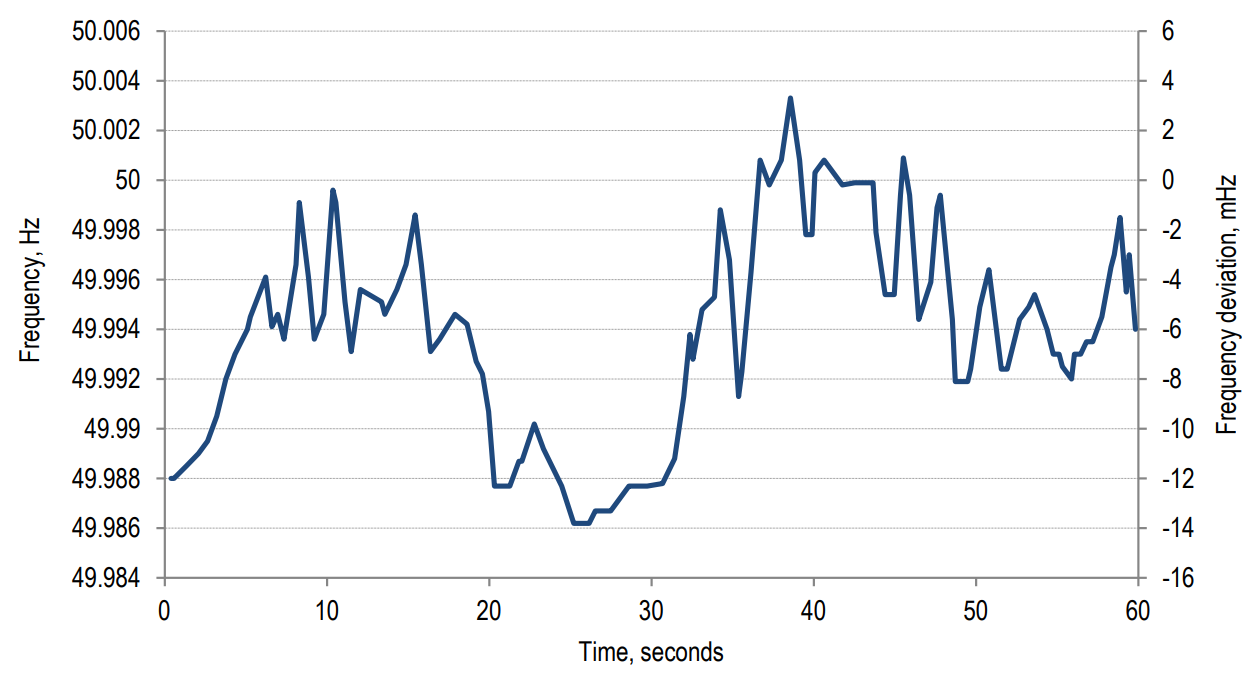
\includegraphics[width=0.7\textwidth]{content/figures/frequency_variation.png}
    \caption{Ejemplo de variaciones en la frecuencia de la red europea (\cite{NEA_2011_load_following}).}
    \label{fig:frequency_variations}
  \end{figure}

  \item \underline{Programas de carga variable predefinidos:} Reducciones o aumentos en la producción de energía acordados previamente con el operador de la red. Se suele tratar de una o dos variaciones de potencia al día, dependiendo de la demanda y de la capacidad de seguimiento de carga de la planta.
  
  \begin{figure}[h]
    \centering
    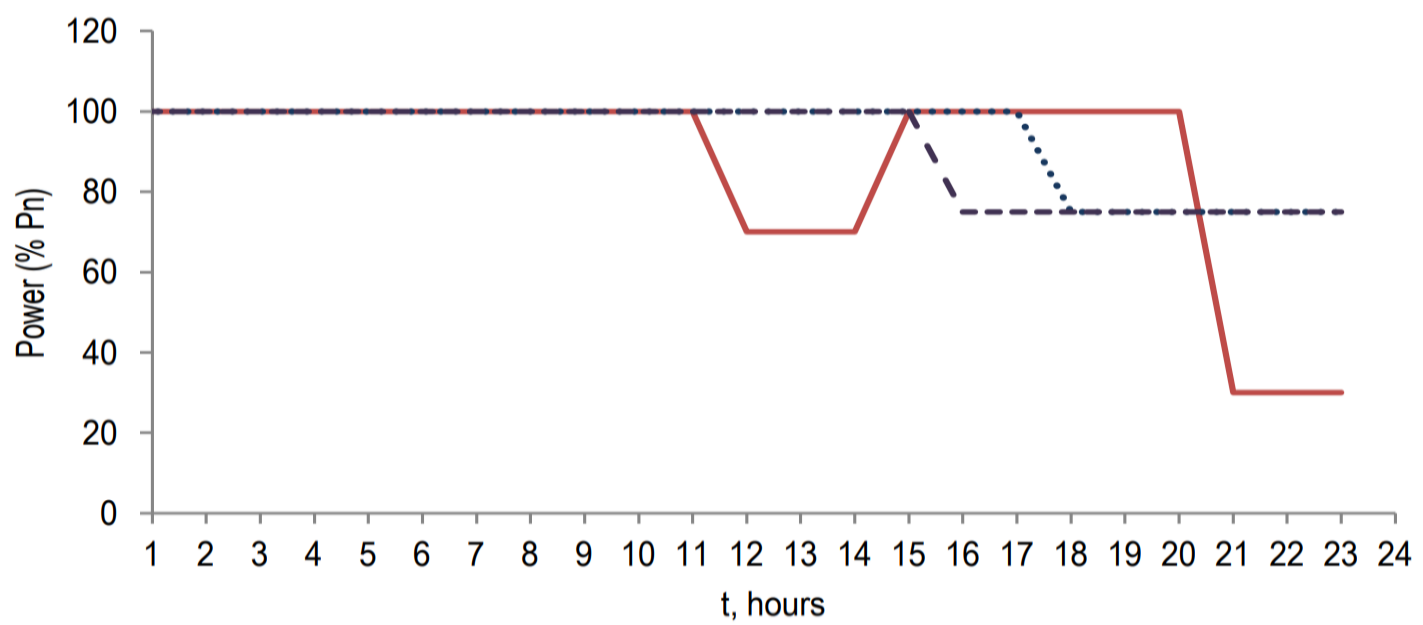
\includegraphics[width=0.7\textwidth]{content/figures/predefined_load_following.png}
    \caption{Ejemplo de un programa de carga variable predefinido para un período de 24 horas, en el que se producen dos reducciones importantes de potencia (\cite{NEA_2011_load_following}).}
    \label{fig:predefined_load_following}
    \vspace{-0.5cm}
  \end{figure}
\end{itemize}

\subsubsection{Capacidades de seguimiento de carga}

Vale la pena tener en cuenta los órdenes de magnitud que muestran cuantitativamente la capacidad de seguimiento de carga de la mayoría de centrales nucleares de gran escala. Estas, se diseñan con una capacidad de seguimiento de carga similar a la de las centrales de carbón, con unas rampas de potencia de entre 1 - 5 \%/min y tiempos de arranque hasta alcanzar la potencia total estable del orden de entre un día y varios días. Estas capacidades de seguimiento de carga son mucho más lentas que las de los generadores de las turbinas de gas, que tienen tiempos de arranque de menos de 1 hora y pueden aumentar la potencia a una tasa del 10-20\%/min (\cite{stanford_load_following}).

Centrando ahora la atención en los \acrlongpl{smr}, destacan sus capacidades avanzadas de seguimiento de carga, las cuales son debidas a diversos aspectos intrínsecos a su tecnología o incorporados intencionadamente para dicho fin:
\begin{itemize}
  \item Su pequeño tamaño permite ajustes más rápidos en la producción eléctrica en comparación con los reactores de gran escala. Esto se debe principalmente a que la inercia térmica del combustible de un reactor más pequeño es menor, lo que permite cambios más rápidos en la potencia del mismo. Además, un menor tamaño del reactor implica que los problemas derivados por la distribución heterogénea del flujo neutrónico a lo largo del núcleo son menos graves que en los reactores más grandes. Aun así, este desequilibrio axial del flujo neutrónico se procura mitigar con venenos consumibles (como el $Gd_2O_3$), venenos solubles (ácido bórico) y con el uso de múltiples bancos de barras de control, incluidas las denominadas ``barras de control grises''\footnote{Las ``barras de control grises'' ---fabricadas por acero y una aleación de Ag, In y Cd---, están diseñadas para absorber una menor cantidad de neutrones, lo cual reduce la deformación de la distribución del flujo neutrónico que se da cuando las barras de control estándar o ``negras'' ---fabricadas por $B_4C$ y una aleación de Ag, In y Cd--- se insertan o se retiran del núcleo.}.
  \item Emplean sistemas de control avanzados y sensores integrados, que proporcionan información en tiempo real sobre las condiciones de la red y facilitan regulaciones rápidas de la producción.
  \item El empleo de sistemas de seguridad pasivos reducen la necesidad de componentes mecánicos activos y permiten transiciones más suaves entre distintos niveles de potencia.
  \item A parte de los puntos anteriores, algunos diseños incorporan características específicamente destinadas a mejorar estas capacidades de seguimiento de carga. Por ejemplo, el empleo de diseños de combustible avanzados que pueden tolerar fluctuaciones de potencia más altas y permitir una operación más estable durante el seguimiento de carga. O el uso de materiales y técnicas de mantenimiento avanzados para mejorar la resistencia y durabilidad de los componentes frente a la corrosión, la fatiga térmica y el desgaste, que se ven acelerados por los cambios de potencia del núcleo.
  \item Por último, los \acrlongpl{smr} con varios módulos tienen una flexibilidad adicional, pudiendo ajustar la producción de energía de forma más precisa y gradual (\cite{smr_load_following_capabilities}).
\end{itemize}

En concreto, los niveles de potencia de los pequeños reactores modulares pueden variar entre el 15 - 100 \%, con rampas de potencia típicas de 2 - 5 \%/min, logrando rampas de potencia de 10 - 20 \%/min en algunos diseños (\cite{ANS_2019}). 

\begin{table}[!h]
  \centering
  \resizebox{0.92\textwidth}{!}{%
  \begin{tabular}{|
    >{\columncolor[HTML]{FFCCC9}}c |c|c|c|}
    \hline
    \cellcolor[HTML]{ECF4FF}\begin{tabular}[c]{@{}c@{}}Tipo de\\ SMR\end{tabular} &
      \cellcolor[HTML]{ECF4FF}\begin{tabular}[c]{@{}c@{}}Potencia eléctrica\\ (MWe)\end{tabular} &
      \cellcolor[HTML]{ECF4FF}\begin{tabular}[c]{@{}c@{}}Rango de potencia\\ (\%)\end{tabular} &
      \cellcolor[HTML]{ECF4FF}\begin{tabular}[c]{@{}c@{}}Rampa de potencia\\ (\%/min)\end{tabular} \\ \hline
    \textit{\begin{tabular}[c]{@{}c@{}}Pressurized Water Reactor\\ (\acrshort{pwr})\end{tabular}}             & 50 - 160   & 20 - 100 \% & 2 - 5 \\ \hline
    \textit{\begin{tabular}[c]{@{}c@{}}Molten Salt Reactor\\ (\acrshort{msr})\end{tabular}}                   & 37,5 - 192 & 20 -100 \%  & 5     \\ \hline
    \textit{\begin{tabular}[c]{@{}c@{}}High Temperature Gas-cooled \\ Reactor (\acrshort{htgr})\end{tabular}} & 76 - 286   & 15 - 100 \% & 5     \\ \hline
    \textit{\begin{tabular}[c]{@{}c@{}}Lead-cooled Fast Reactor\\ (\acrshort{lfr})\end{tabular}}              & 3 - 450    & 0 - 125 \%  & 10    \\ \hline
    \textit{\begin{tabular}[c]{@{}c@{}}Sodium Fast Reactor\\ (\acrshort{sfr})\end{tabular}}                   & 50 - 311   & 20 - 100 \% & 1 - 2 \\ \hline
    \textit{\begin{tabular}[c]{@{}c@{}}Heat Pipe cooled Reactor\\ (\acrshort{hpr})\end{tabular}}              & 0,2 - 25   & 60 - 100 \% & 20    \\ \hline
    \end{tabular}
  }
  \caption{Capacidad de seguimiento de carga de 16 diseños distintos de \acrshortpl{smr} agrupados en el tipo de SMR al que pertenece cada diseño (\cite{ANS_2019}).}
  \label{tab:capacidad_seguimiento_de_carga_smrs}
  \end{table}

  \subsubsection{Métodos para el seguimiento de carga} \label{metodos_seguimiento_de_carga}

  Es importante tener en cuenta que las maniobras de variación de potencia se realizan de acuerdo con el criterio \textit{reactor sigue a turbina}, por lo que se actúa sobre la turbina y no directamente sobre el reactor. La potencia que suministra la turbina depende del gasto másico de vapor y del salto entálpico ---que, a su vez, depende de las condiciones termodinámicas del vapor a la entrada y a la salida de la turbina---. Por tanto, para variar la potencia es necesario modificar el gasto de vapor, lo cual se realiza actuando sobre las válvulas de regulación de la turbina. Estas, se abren o se cierran ---dejando pasar un mayor o menor gasto de vapor--- según se quiera aumentar o reducir la potencia, respectivamente (\cite{apuntes_centrales}). Como consecuencia de esta maniobra, se producen cambios en otras magnitudes, que serán las señales de actuación sobre distintos sistemas de control, que procurarán acomodar la planta a la nueva situación mediante los siguientes mecanismos:

\begin{itemize}
  \item \underline{Variación en la concentración de ácido bórico:} Se emplea en los reactores \acrshort{pwr} y el principal problema de este mecanismo es que se trata de un proceso lento que requiere de varios minutos para tener efecto. Por ello, este método se emplea para los cambios de potencia programados y no para cambios rápidos, para los cuales son más apropiados los dos métodos que se detallan a continuación. Obviamente, también puede usarse este método para variaciones de potencia no programadas, siempre y cuando el tiempo requerido para las mismas sea, al menos, de unos minutos.
  
  \item \underline{Empleo de bancos especiales de las barras de control:} 
  Se trata, concretamente, de los bancos de barras de control A, B, C y D, los cuales se denominan ``bancos de control u operación''.

  Están presentes en todos los tipos de reactores, siendo la forma más común de ajustar la potencia. Las ventajas que presenta el empleo de las barras de control es que ofrecen una respuesta rápida y pueden adaptarse a sistemas de control automático. Sin embargo, producen una distorsión en la distribución del flujo neutrónico y, por tanto, de la potencia, ya que se agota más el combustible en la parte inferior del reactor que en la parte superior, por donde se insertan dichas barras en el caso de los \acrshortpl{pwr}. Este problema puede corregirse variando la concentración de ácido bórico y retirando después las barras de control (\cite{apuntes_centrales}).

  \item \underline{Empleo del coeficiente de temperatura del moderador:} Este coeficiente representa la variación de la \gls{reactividad}\footnote{Capacidad que tiene el reactor de multiplicar la población neutrónica. Según el valor de la reactividad $(\rho)$, el sistema será subcrítico $(\rho<0)$, crítico $(\rho=0)$ o supercrítico $(0<\rho<1)$. Siempre se busca alcanzar y mantener la criticidad $(\rho=0)$ para que la reacción de fisión nuclear en cadena se automantenga de forma controlada.} con la temperatura del moderador: 
  
  \begin{equation}
    \alpha_{mod}=\frac{\partial \rho}{\partial T_{mod}}
  \end{equation}

  Un reactor, para ser intrínsecamente estable ---y, por tanto, seguro---, debe tener un coeficiente de potencia negativo, de modo que un aumento en la \gls{reactividad} del núcleo conlleve una reducción de la potencia, tal y como se muestra a continuación:

  \begin{equation} \label{coeficiente_potencia}
    \frac{\partial \rho}{\partial P}=\frac{\partial \rho}{\partial T_c} \frac{\partial T_c}{\partial P}+\frac{\partial \rho}{\partial T_{\mathrm{mod}}} \frac{\partial T_{\mathrm{mod}}}{\partial P}=\alpha_{T c} \frac{\partial T_c}{\partial P}+\alpha_{\mathrm{mod}} \frac{\partial T_{\mathrm{mod}}}{\partial P}<0
  \end{equation}

  Como las temperaturas del combustible y del moderador aumentan con la potencia ($\frac{\partial T_c}{\partial P}>0, \frac{\partial T_{\mathrm{mod}}}{\partial P}>0$), es necesario que el coeficiente Doppler ($\alpha_{T_{c}}$) y el coeficiente de temperatura del moderador ($\alpha_{mod}$) sean negativos. En un reactor con coeficiente de temperatura del moderador negativo ---para lo cual debe diseñarse para operar en régimen de submoderación---, un aumento de temperatura del moderador conlleva una disminución de la \gls{reactividad} y, por la ecuación \ref{coeficiente_potencia}, una consecuente disminución de la potencia. De esta manera, aumentando la temperatura del moderador o sobrerrefrigerando el núcleo se disminuye o aumenta, respectivamente, la potencia de la planta (\cite{apuntes_centrales}).
  
  Las ventajas que presenta este método es que no hace uso de materiales que puedan desgastarse y que proporciona una potencia homogénea en todo el reactor. Sin embargo, si los cambios de potencia ---y, por tanto, de temperatura--- son muy bruscos, será necesario un presionador lo suficientemente grande como para adaptar la presión del circuito primario a los cambios del nivel de agua producidos (\cite{seguimiento_carga_josep_rey}).
\end{itemize}

Es importante destacar que la capacidad de seguimiento de carga de la central se ve significativamente influenciada por el momento del ciclo en el que se encuentre la misma. Hacia el final del ciclo, debido al mayor quemado del combustible, su reactividad es menor, lo cual disminuye, por ejemplo, la velocidad de subida de potencia al extraer parcialmente las barras de control o diluir el ácido bórico, en caso de que nos interese incrementar la potencia. Asimismo, en esas condiciones existe muy poco margen de variación de la concentración de ácido bórico, lo que también hace menos flexible el seguimiento de carga (\cite{apuntes_centrales}).

En la figura \ref{fig:seguimiento_carga_barras_y_boro} se muestra una operación de variación de potencia en que se emplean los dos primeros métodos explicados.

\begin{figure}[h]
  \centering
  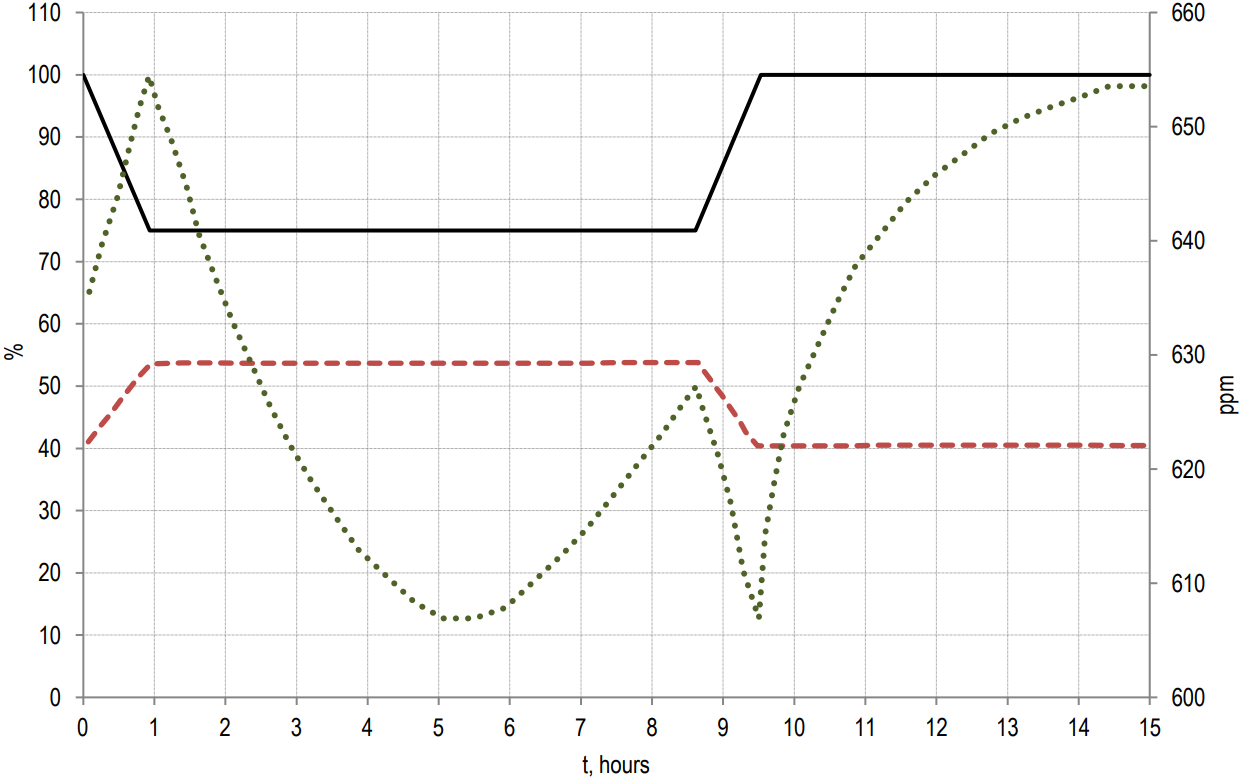
\includegraphics[width=0.7\textwidth]{content/figures/seguimiento_carga_barras_y_boro.png}
  \caption{Ejemplo de variación de potencia mediante la inserción del banco de barras de control D y la variación de la concentración de ácido bórico en un reactor \acrshort{pwr} (\cite{NEA_2011_load_following}).}
  \label{fig:seguimiento_carga_barras_y_boro}
\end{figure}

Tal y como se ha comentado al inicio de este subapartado, es preferible mantener el reactor operando constantemente a su máxima potencia, evitando así el ciclado térmico de los componentes del núcleo del reactor y del circuito primario. Por eso, los diseños de \acrshort{smr} más recientes apuestan principalmente por mantener siempre el circuito primario de la planta a plena potencia y seguir la curva de carga utilizando la energía ---tanto térmica como eléctrica--- del lado secundario para la cogeneración Una opción muy atractiva es la derivación de vapor sin pasar por la turbina. Cuando la demanda de electricidad en la red eléctrica cambia, el operador de la central puede ajustar la cantidad de vapor que pasa a través de la turbina principal utilizando válvulas de derivación. Al abrirlas, parte del vapor se desvía y no pasa por la turbina, lo que reduce la cantidad de energía que se convierte en electricidad (\cite{ANS_2019}). Este vapor puede emplearse para distintos fines, como calefacción urbana, desalación, producción de hidrógeno, etc. tal y como se detalla en el apartado de \textit{Cogeneración (\ref{cogeneracion})}. 

\subsubsection{Efectos del xenón ante variaciones de potencia}

Durante la operación de un reactor nuclear se acumula una gran cantidad de productos de fisión. Entre ellos, hay que prestar especial atención al $Xe^{135}$, cuya sección eficaz de captura neutrónica en el rango térmico es muy elevada, actuando como ``veneno del reactor'' e introduciendo reactividad negativa al mismo. El efecto de este envenenamiento ---que se pone especialmente de manifiesto en las operaciones de arranque, parada y variaciones de potencia--- debe tenerse muy en cuenta a la hora de diseñar y operar un reactor térmico.

El $Xe^{135}$ aparece directamente como un producto de fisión y por desintegración del $I^{135}$. A su vez, desaparece por captura y por decaimiento.

\begin{figure}[h]
  \centering
  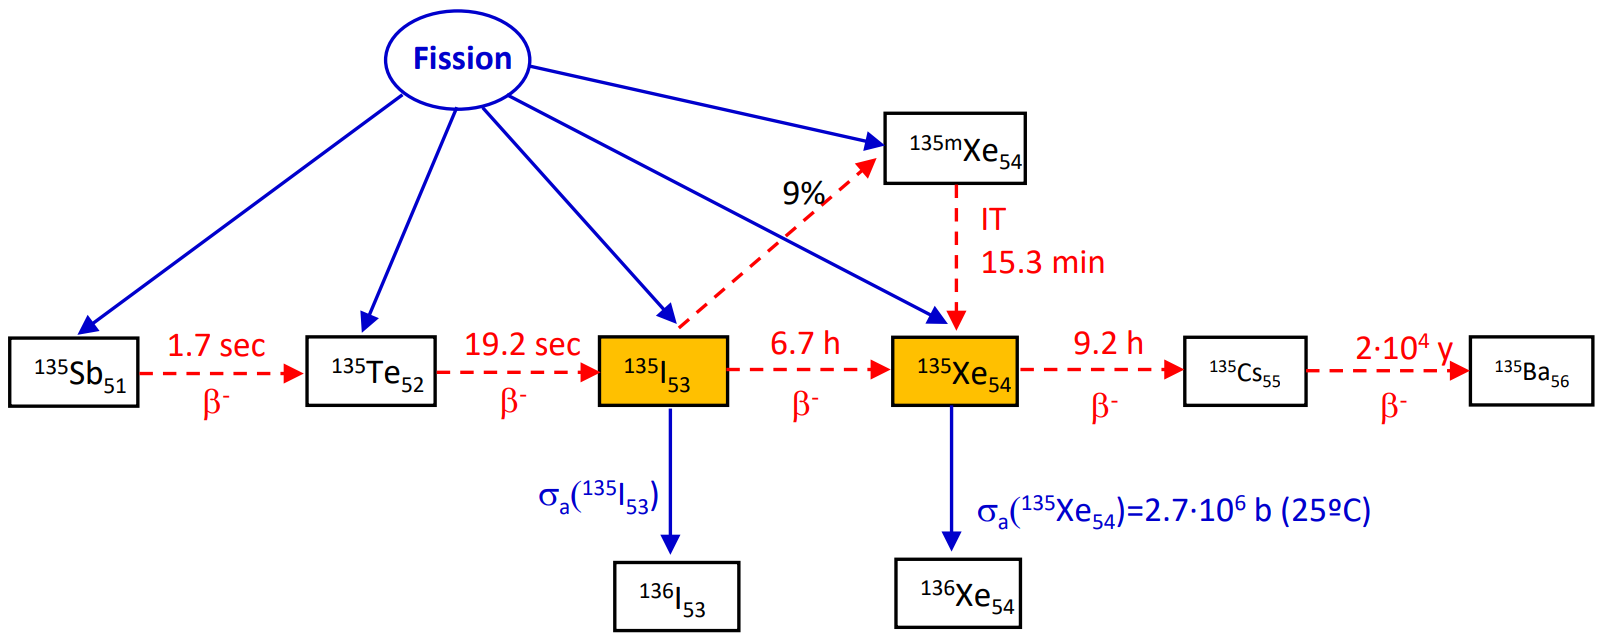
\includegraphics[width=0.8\textwidth]{content/figures/esquema_xenon.png}
  \caption{Esquema completo de aparición y desaparición del $Xe^{135}$ (\cite{apuntes_centrales}).}
  \label{fig:esquema_xenon}
\end{figure}

Asumiendo que las desintegraciones del $Te^{135}$ y del $Sb^{135}$ son instantáneas ---y se combinan los rendimientos de fisión en los denominados \textit{rendimientos de fisión acumulados ($\gamma$)}---, que el decaimiento del $Cs^{135}$ es despreciable y que la absorción del $I^{135}$ es despreciable comparada con su decaimiento, se obtiene el esquema simplificado de aparición y desaparición del $Xe^{135}$ mostrado en la figura \ref{fig:esquema_xenon_simplificado}, con la evolución temporal de la ecuación \ref{evolucion_xenon}:

\begin{figure}[!h]
  \centering
  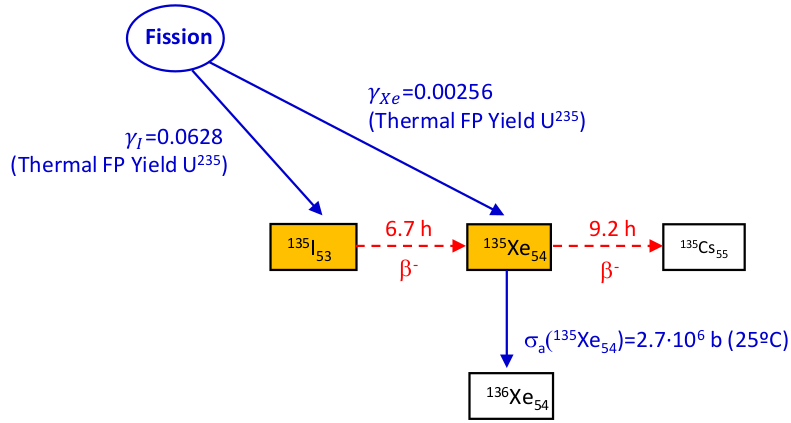
\includegraphics[width=0.6\textwidth]{content/figures/esquema_xenon_simplificado.png}
  \caption{Esquema simplificado de aparición y desaparición del $Xe^{135}$ (\cite{apuntes_centrales}).}
  \label{fig:esquema_xenon_simplificado}
\end{figure}

\begin{equation} \label{evolucion_xenon}
  \frac{d X e}{d t}=\gamma_{X e} \cdot \Sigma_f \cdot \Phi+\lambda_I \cdot I-\left(\lambda_{X e}+\sigma_a^{X e} \cdot \Phi\right) \cdot X e
\end{equation}

En lo que respecta al seguimiento de carga, interesa conocer la evolución del xenón tras los cambios de potencia. 

En primer lugar, hay que tener en cuneta que el principal término fuente del $Xe^{135}$ es el decaimiento del $I^{135}$ y que el principal término sumidero es la captura. Analizando la ecuación \ref{evolucion_xenon} puede observarse que una disminución del flujo neutrónico ($\phi$) ---en el caso de una disminución de potencia del reactor--- implica la reducción del término sumidero de  $Xe^{135}$, lo que conlleva un incremento en la cantidad del mismo no indefinido, ya que pasado un tiempo el xenón alcanza un nuevo estado de equilibrio. Por otro lado, un aumento en el flujo neutrónico ---en el caso de un aumento dee la potencia del reactor--- conlleva una consecuente disminución en la cantidad de $Xe^{135}$. Estas fluctuaciones en la cantidad de xenón inducen transitorios de reactividad que
originan oscilaciones espacio-temporales del flujo neutrónico en reactores con flujos elevados.

\begin{figure}[h]
  \centering
  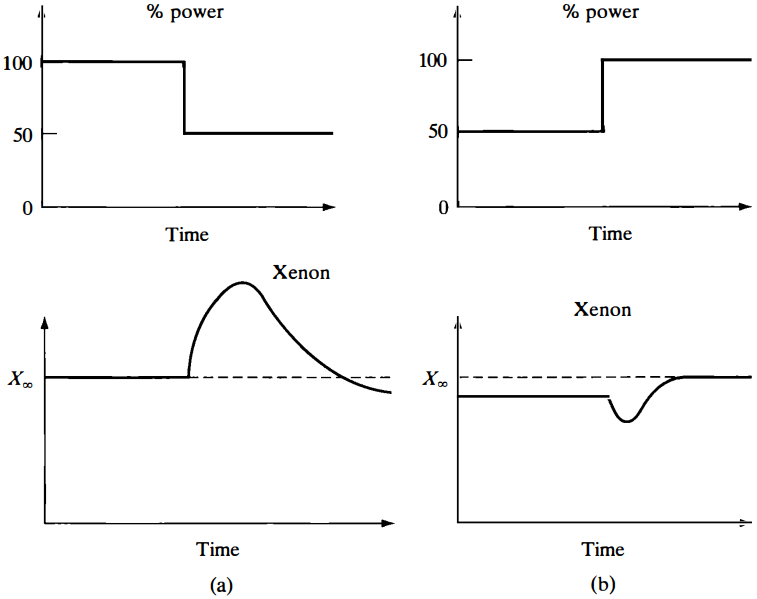
\includegraphics[width=0.62\textwidth]{content/figures/variaciones_potencia_xenon.png}
  \caption{Variaciones de la cantidad de $Xe^{135}$ al producirse variaciones en el flujo neutrónico (\cite{intro_nuclear_engineering}).}
  \label{fig:variaciones_potencia_xenon}
\end{figure}

\subsection{Simulación de una maniobra de seguimiento de carga de corta duración. Implementación como práctica académica}

La primera simulación realizada consiste en una maniobra de seguimiento de carga en la que se pasa del 100\% de potencia al 50\% y, tras un periodo de estabilización, se vuelve a aumentar la potencia hasta el valor nominal.

Esta primera simulación permite analizar y comprender ---en un tiempo de realización corto--- varios aspectos relevantes de la operación de los reactores nucleares durante una maniobra de seguimiento de carga, centrando la atención en el caso de los \acrshortpl{smr}. Esta es la razón por la que se ha decidido implementar la simulación como práctica académica.

De esta manera, la explicación detallada de la simulación, junto con la exposición y el análisis de los resultados, se muestra en el siguiente apartado. En él, se incluye una parte del guión que se entrega a los alumnos antes de la realización de la práctica. Se ha omitido la introducción teórica al seguimiento de carga, que ya se ha explicado en el apartado \ref{seguimiento_de_carga} de esta memoria. Además, se incluyen las respuestas a las cuestiones planteadas en el guión, donde se comentan detalladamente las gráficas obtenidas.

\subsubsection{Guión de la práctica de seguimiento de carga} \label{sec:anexo1}

\begin{itemize}
    \item \textbf{Título:} Simulación de una maniobra de seguimiento de carga de un \acrshort{smr} con el \acrshort{sgiz}.
    \item \textbf{Duración aproximada:} 2 horas.
    \item \textbf{Lugar de realización:} \acrfull{sgiz} de la Escuela Técnica Superior de Ingenieros Industriales (UPM).
    \item \textbf{Impartición:} Alumnos de la asignatura de \textit{Tecnologías Avanzadas en Reactores Nucleares} del \textit{Máster en Ciencia y Tecnología Nuclear}.
\end{itemize}

\paragraph{Objetivo de la simulación}

El objetivo de esta práctica es simular una maniobra de seguimiento de carga con el fin de adaptarse a las fluctuaciones de la energía eólica y solar en un período de tiempo concreto. Una vez realizada la simulación, el simulador ofrece las gráficas y tablas de datos necesarias para analizar el funcionamiento de la planta durante ese modo de operación. Por último, debido a que la Central Nuclear de Zorita es de un solo lazo y produce 150 MWe de potencia ---características típicas de algunos \acrshortpl{smr}---, se pretende analizar la capacidad de seguimiento de carga de esta central y compararla con la que puede tener un \acrshort{smr}.

\paragraph{Contextualización}

El caso concreto en el que se contextualiza la simulación es una tarde de agosto muy soleada y con muy poco viento en la que, a las 20.00, llegan de repente fuertes vientos a la península y la producción eólica aumenta drásticamente. La central baja en unos 15 minutos la producción de potencia al 50\% y, tras permanecer unos 10 minutos a dicho nivel de producción, comienza a atardecer a las 20.30, disminuyendo rápidamente la producción solar. Ante esto, la central vuelve a subir ---en otros 15 minutos aproximadamente--- la potencia hasta el 100\%, nivel de producción al que se mantendrá toda la noche debido a la falta de producción solar.

\paragraph{Procedimiento} \label{procedimiento}

Dado que en esta simulación se trabajará con valores de potencia dentro del rango entre el 15 - 100 \%\footnote{Por debajo del 15\% de potencia, las actuaciones deberían hacerse en \textit{modo manual}.}, la central trabajará en \textit{modo automático}. En este modo, el sistema de control del reactor permite a la central adaptarse automáticamente a variaciones de potencia del 3\% por minuto y a cambios bruscos del 5\% (ritmos superiores supondrían un elevado estrés térmico). 

Durante toda la simulación es importante comprobar que la diferencia entre la temperatura media del primario ($T_{med}$) y la temperatura de referencia\footnote{Temperatura teórica que determina, para cada caudal de vapor, la temperatura media que debería haber en el primario para que la potencia nuclear se adapte a la potencia demandada por la turbina.} ($T_{ref}$) es inferior a 2ºC, asegurando así el funcionamiento estable del reactor. En caso de que en algún momento no se cumpla este requisito, disminuir ligeramente la tasa de variación de potencia.

A continuación se detallan los pasos a seguir en el transcurso de la simulación:

\begin{enumerate}
  \item Una vez encendido y ejecutado el simulador, cargar la condición inicial 51: \textit{100\% \acrshort{bol} nuevos coeficientes de reactividad}.
  
  \item Los sistemas involucrados en un transitorio de variación de carga son, principalmente, el circuito primario y el secundario. Por tanto, es suficiente con abrir las siguientes dos pantallas:
  \begin{itemize}
    \item \textbf{Pantalla NSSS-SI-AFW:} Circuito primario. Principales componentes de interés: lazo del primario, reactor, presionador (PZR) y generador de vapor (GV).
    \item \textbf{Pantalla MS-MSR-GS-TU-OPC-LO:} Circuito secundario. Componentes de interés: controlador del límite de carga y válvulas de regulación (1, 2, 3 y 4).
    \end{itemize}

  \begin{figure}[h!]
    \centering
    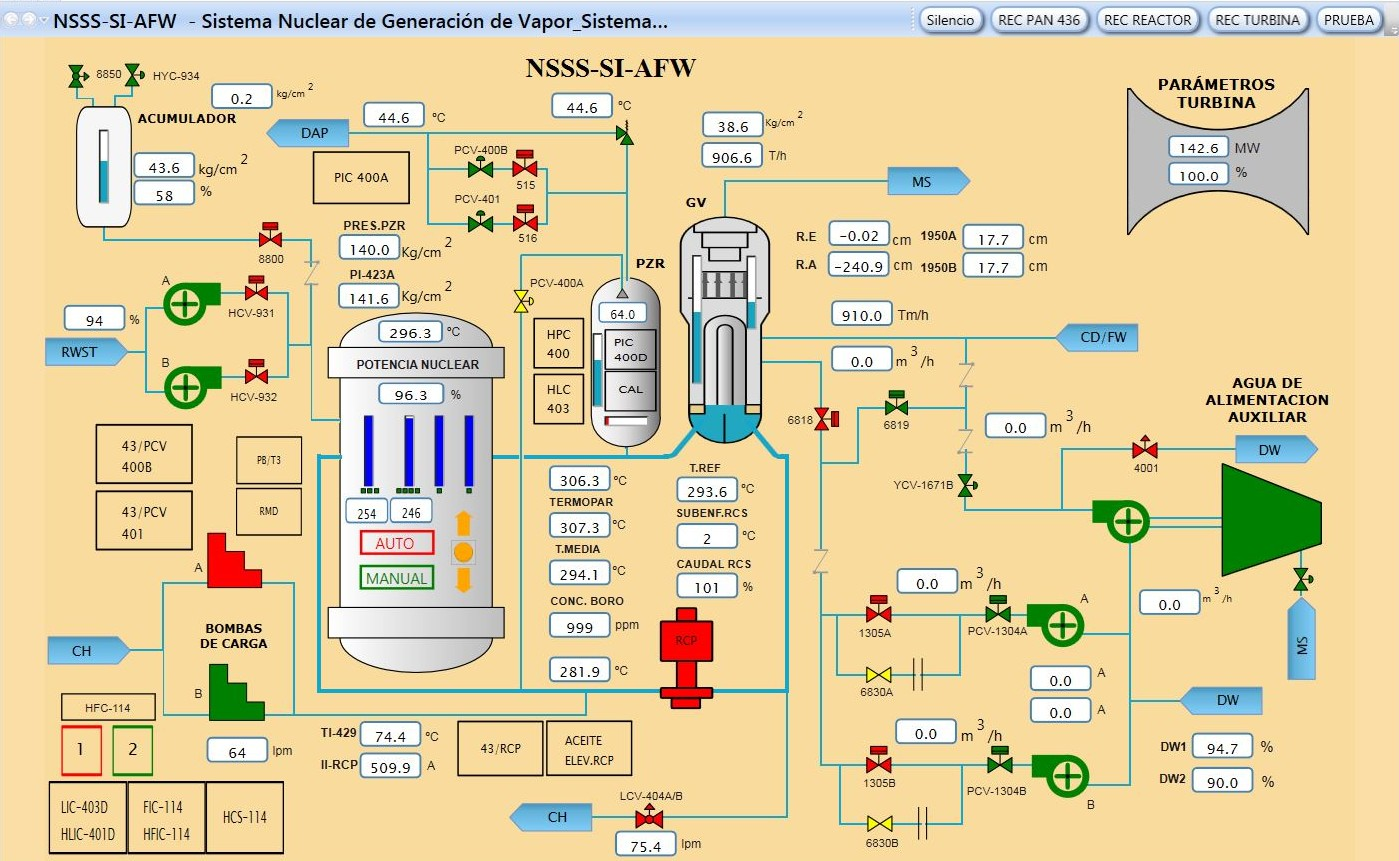
\includegraphics[width=0.85\textwidth]{content/figures/pantalla1_simulacion1.JPG}
    \caption{Pantalla NSSS-SI-AFW correspondiente al momento inicial de la simulación.}
    \label{fig:pantalla1_simulacion1}
  \end{figure}

  \begin{figure}[h!]
    \centering
    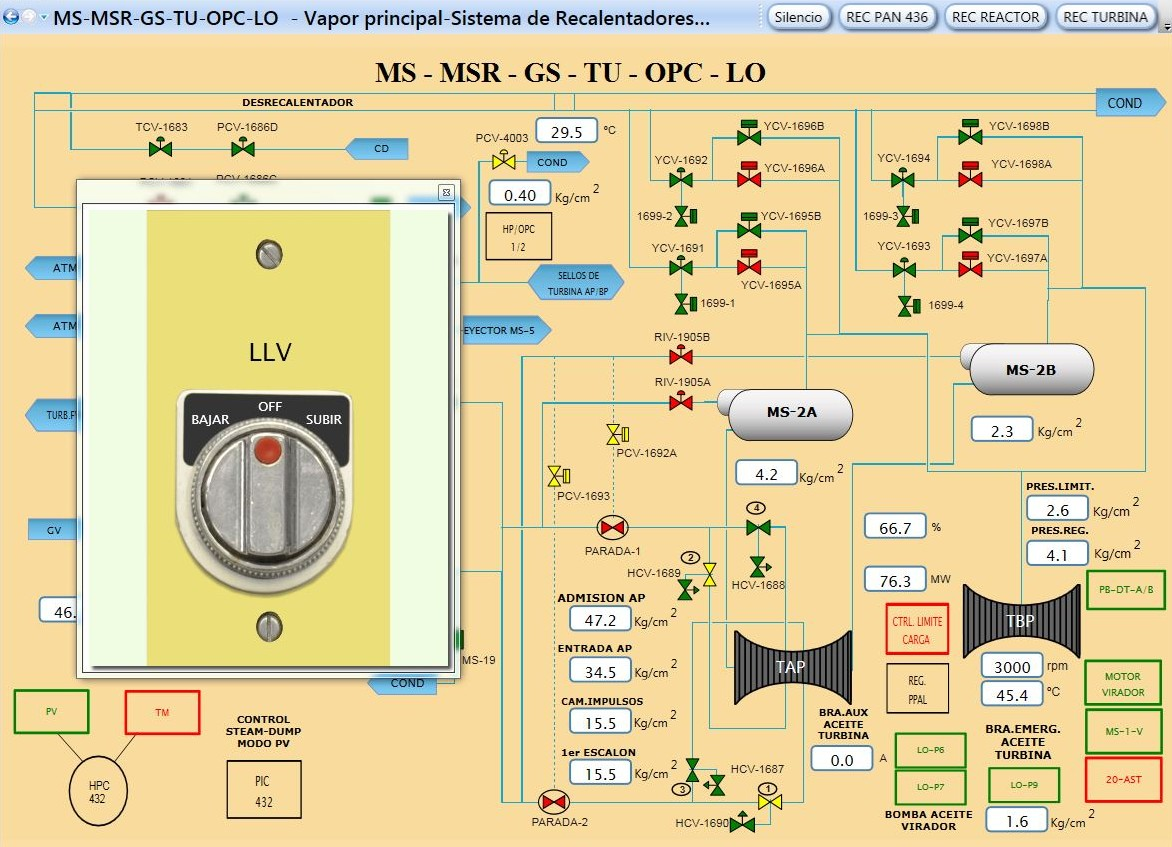
\includegraphics[width=0.75\textwidth]{content/figures/pantalla2_simulacion2.JPG}
    \caption{Pantallas MS-MSR-GS-TU-OPC-LO correspondiente a una fase intermedia de la simulación.}
    \label{fig:pantalla2_simulacion1}
  \end{figure}

  \item Iniciar la simulación y comenzar las bajadas de potencia pulsando ``BAJAR'' en el controlador del límite de carga en la pantalla MS-MSR-GS-TU-OPC-LO. Realizar bajadas del 3\% en turbina y esperar 1 minuto y medio para que se estabilice el sistema en cada una de ellas. 
  \item Realizar el proceso anterior de bajada hasta alcanzar el 50\% de potencia nuclear. Una vez llegados a este punto, mantener el nivel de potencia durante 10 minutos.
  \item Pasados los 10 minutos de estabilización, realizar las necesarias subidas de potencia pulsando el botón ``SUBIR'' del controlador del límite de carga. Igual que en el paso 3, realizar subidas del 3\% en turbina y esperar 1 minuto y medio tras cada una de ellas.
  \item Una vez alcanzado el 100\% de potencia nuclear, esperar 2 minutos para que se estabilice el sistema y finalizar la simulación.
\end{enumerate}  

\paragraph{Resultados y cuestiones}

\begin{enumerate}
  \item Emplear la funcionalidad \textit{Gráfico de tendencias} del simulador para tabular y graficar los siguientes parámetros en función del tiempo de la operación:
    \begin{itemize}
      \item \underline{Gráfica 1 - Variaciones de potencia}
      \begin{itemize}
        \item Potencia nuclear
        \item Potencia activa del generador principal
      \end{itemize}
      \item \underline{Gráfica 2 - Variaciones de temperatura}
      \begin{itemize}
        \item Temperatura media
        \item Temperatura de referencia
      \end{itemize}
      \item \underline{Gráfica 3 - Posición del las válvulas de control de la turbina}
      \begin{itemize}
        \item Posición de la válvula de control 1
        \item Posición de la válvula de control 2
        \item Posición de la válvula de control 3
        \item Posición de la válvula de control 4
      \end{itemize}
      \item \underline{Gráfica 4 - Caudal de vapor}
      \item \underline{Gráfica 5 - Inserción de las barras de control}
      \begin{itemize}
        \item Pasos extraídos del banco de control 1
        \item Pasos extraídos del banco de control 2
      \end{itemize}
      \item \underline{Gráfica 6 - Concentración de boro}
      \item \underline{Gráfica 7 - Parámetros del presionador}
      \begin{itemize}
        \item Presión del presionador
        \item Nivel del presionador 
        \item Caudal de descarga
      \end{itemize}
      \item \underline{Gráfica 8 - Parámetros del generador de vapor}
      \begin{itemize}
        \item Presión del generador de vapor
        \item Nivel del generador de vapor (rango estrecho)
        \item Presión de la cámara de impulsos
      \end{itemize}
    \end{itemize}
  \vspace{1cm}
  \item Responder a las siguientes cuestiones sobre las gráficas previamente obtenidas:
  \begin{itemize}
    \item \underline{Cuestión gráficas 1 y 2:} ¿A qué se deben los ligeros picos de potencia que se dan en la curva de \textit{potencia nuclear}? ¿Tienen alguna relación con los picos que se dan en la curva de \textit{temperatura media}?
    \item \underline{Cuestión gráfica 5:} ¿A qué parámetro físico del reactor responde el sistema de control automático cuando inserta o extrae las barras de control?
    \item \underline{Cuestión gráfica 6:} A parte de aportar reactividad negativa cuando es necesario, pese al inconveniente de su lentitud, ¿qué ventaja presenta la inyección de ácido bórico para apoyar en las variaciones de potencia?
    \item \underline{Cuestión gráficas 7 y 8:} Razonar en un breve párrafo el comportamiento de los distintos parámetros graficados del generador de vapor y del presionador.
  \end{itemize}

  \item Completar la tabla \ref{tab:resultados_simulacion1} y, tras observar la tabla \ref{tab:capacidad_seguimiento_de_carga_smrs} y las figuras \ref{fig:seguimiento de carga_smr} y \ref{fig:sim2_potencias}, contestar a la siguiente cuestión:
  \begin{itemize}
    \item \underline{Cuestión \acrshortpl{smr}:} ¿Se puede decir que la capacidad de seguimiento de carga de la Central Nuclear de Zorita es similar a la de algunos \acrshortpl{smr}?
  \end{itemize}
  \begin{table}[h]
    \centering
    \resizebox{1\textwidth}{!}{%
    \begin{tabular}{|c|c|c|c|c|c|c|}
      \hline
      \rowcolor[HTML]{ECF4FF} 
      \textbf{\begin{tabular}[c]{@{}c@{}}Potencia inicial\\ (MWe generados\\  y \% nuclear)\end{tabular}} &
        \textbf{\begin{tabular}[c]{@{}c@{}}Potencia intermedia\\ (MWe generados\\  y \% nuclear)\end{tabular}} &
        \textbf{\begin{tabular}[c]{@{}c@{}}Duración bajada\\ de potencia\\ (min)\end{tabular}} &
        \textbf{\begin{tabular}[c]{@{}c@{}}Rampa media de \\ potencia en la bajada\\ (\%/min)\end{tabular}} &
        \textbf{\begin{tabular}[c]{@{}c@{}}Potencia final\\ (MWe generados\\  y \% nuclear)\end{tabular}} &
        \textbf{\begin{tabular}[c]{@{}c@{}}Duración subida\\ de potencia \\ (min)\end{tabular}} &
        \textbf{\begin{tabular}[c]{@{}c@{}}Rampa media de \\ potencia en la subida \\ (\%/min)\end{tabular}} \\ \hline
      \cellcolor[HTML]{FFFFFF}\textit{} &
         &
         &
         &
         &
         &
         \\ \hline
      \end{tabular}
    }
    \caption{Principales resultados de la maniobra de seguimiento de carga.}
    \label{tab:resultados_simulacion1}
    \end{table}

    \begin{figure}[h]
      \centering
      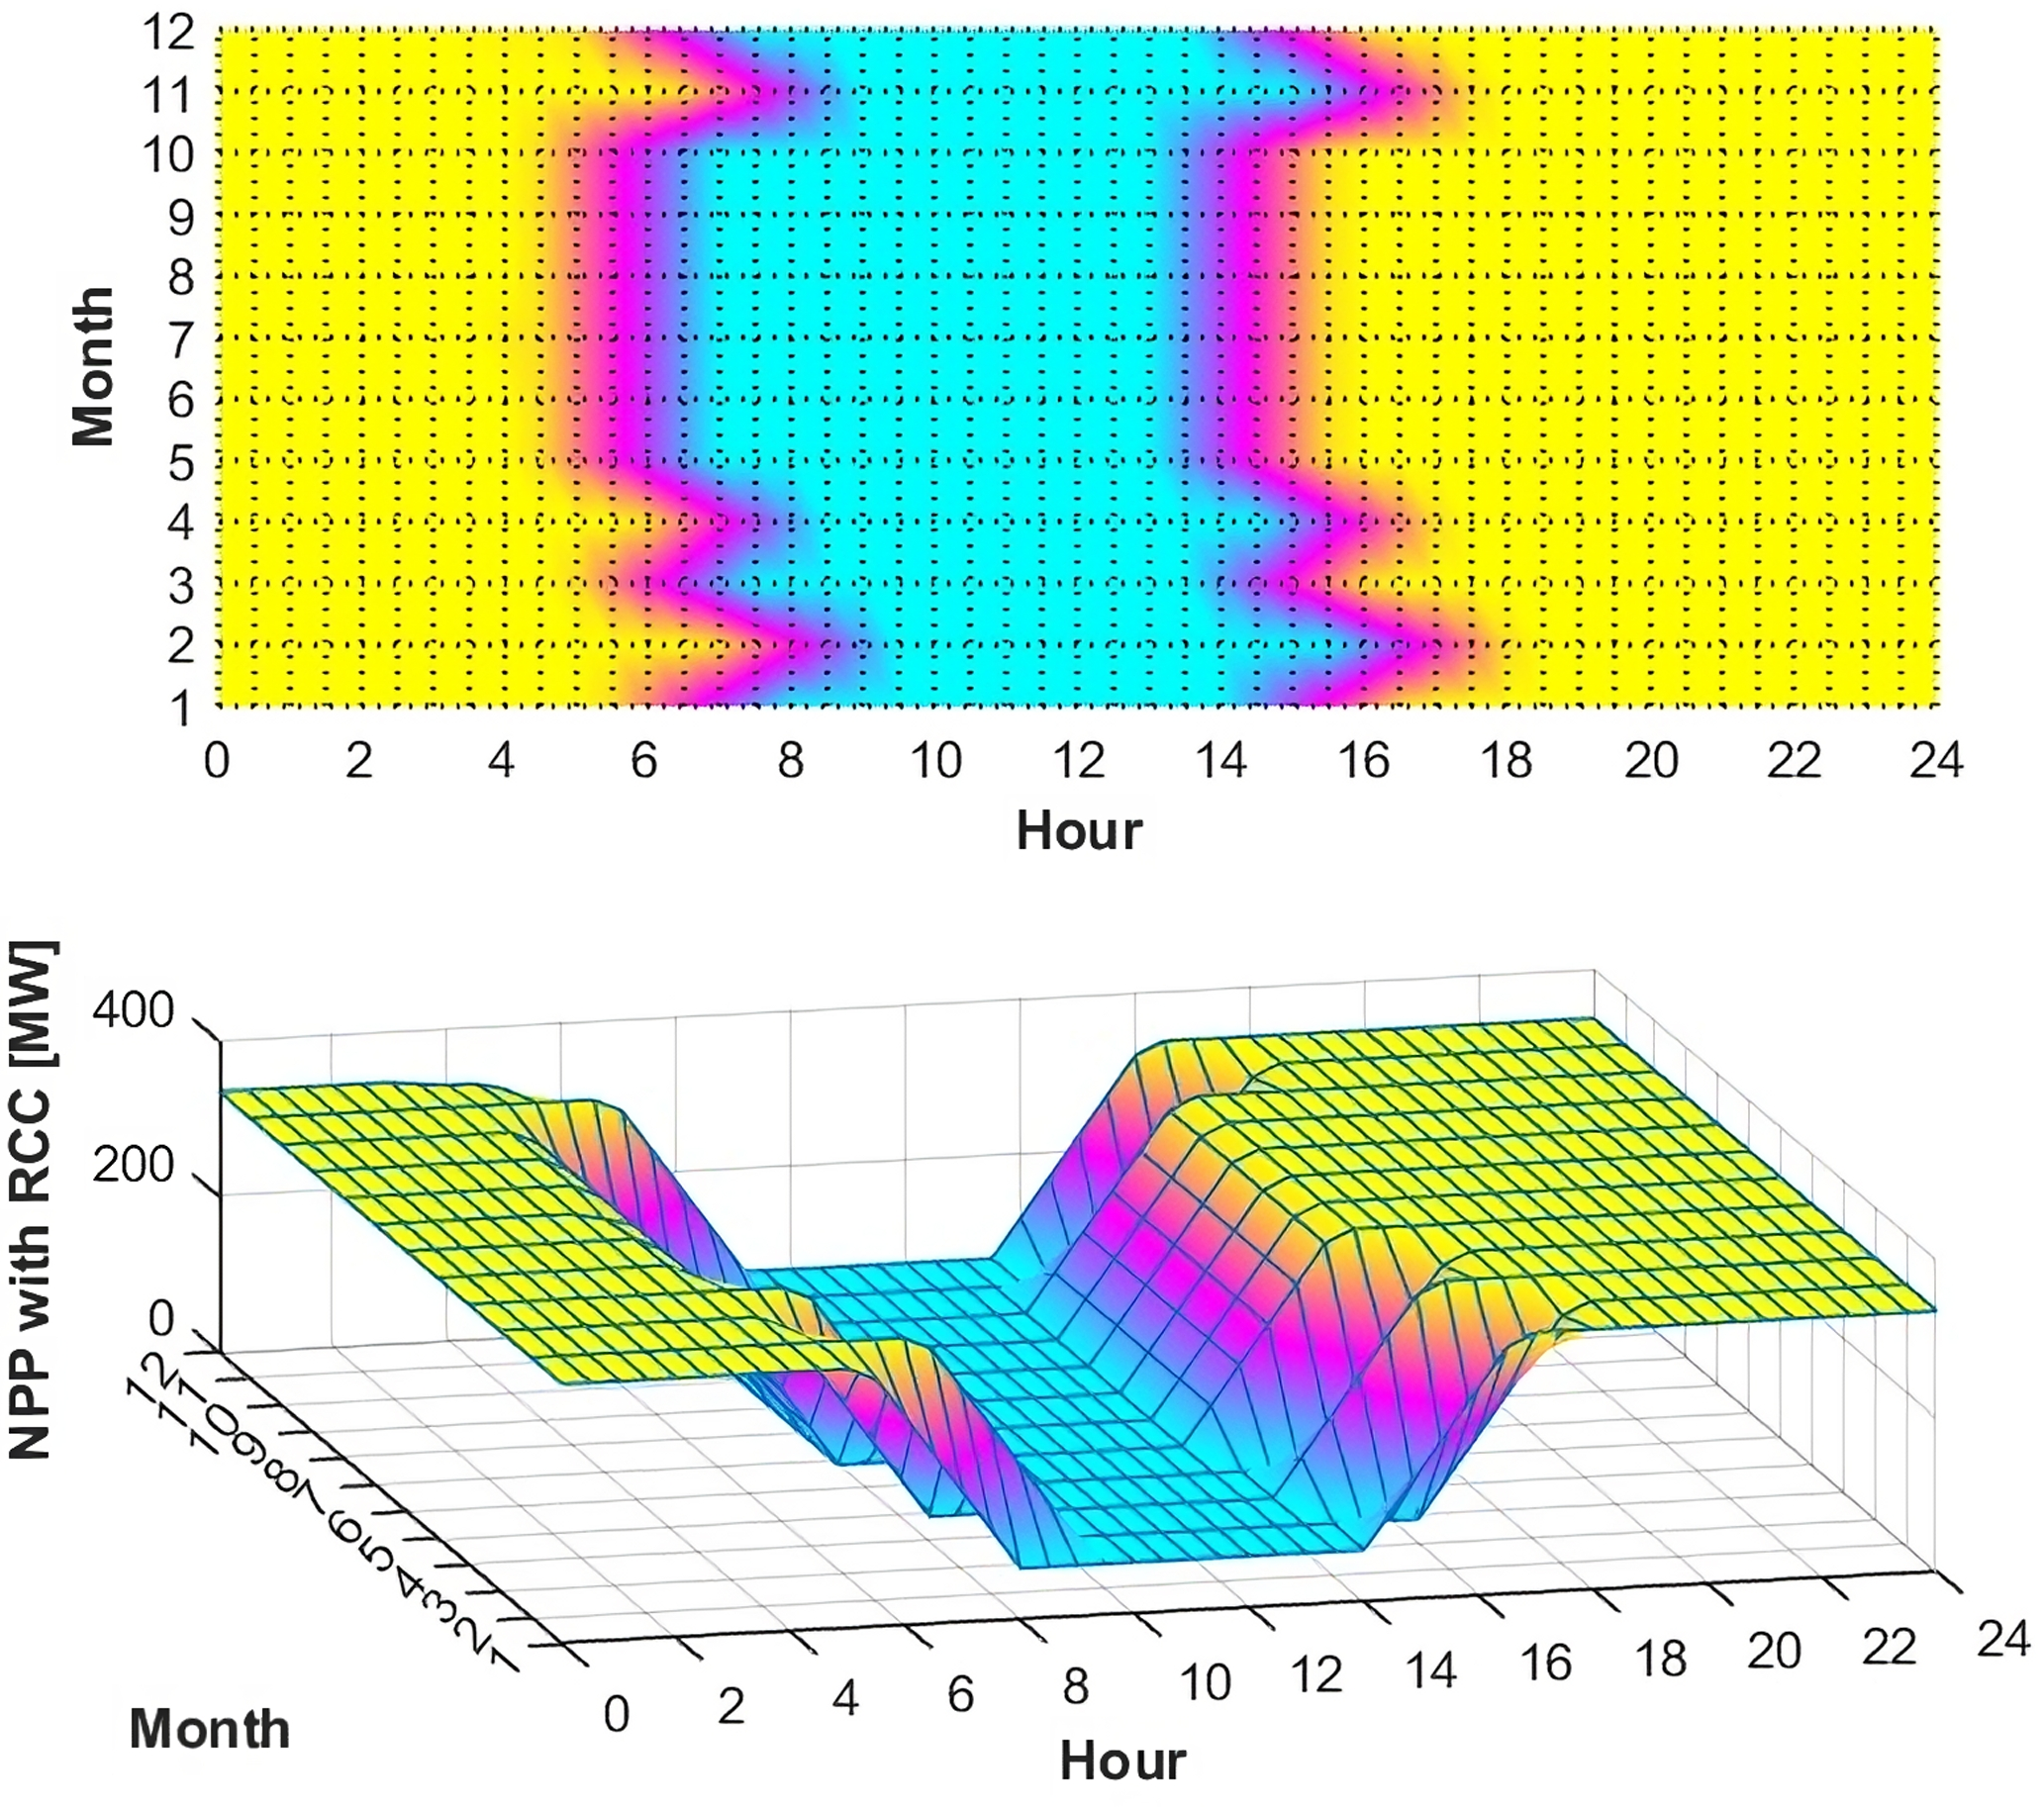
\includegraphics[width=0.75\textwidth]{content/figures/seguimiento_carga_smr.png}
      \caption{Estudio del seguimiento de carga (100 - 20 - 100\%) de un \acrshort{smr} de 335 MWe, adaptándose a las horas de máxima producción solar de los distintos meses del año en Seúl. Tasa de variación de carga: 1,25\%/min. \textbf{Color amarillo} = máxima potencia (335 MWe). \textbf{Color azul} = 67 MWe (20\% de potencia). \textbf{Color violeta} = rampas de potencia (\cite{SMRs_load_following_PV}).}
      \label{fig:seguimiento de carga_smr}
    \end{figure} 

    \begin{figure}[h!]
      \centering
      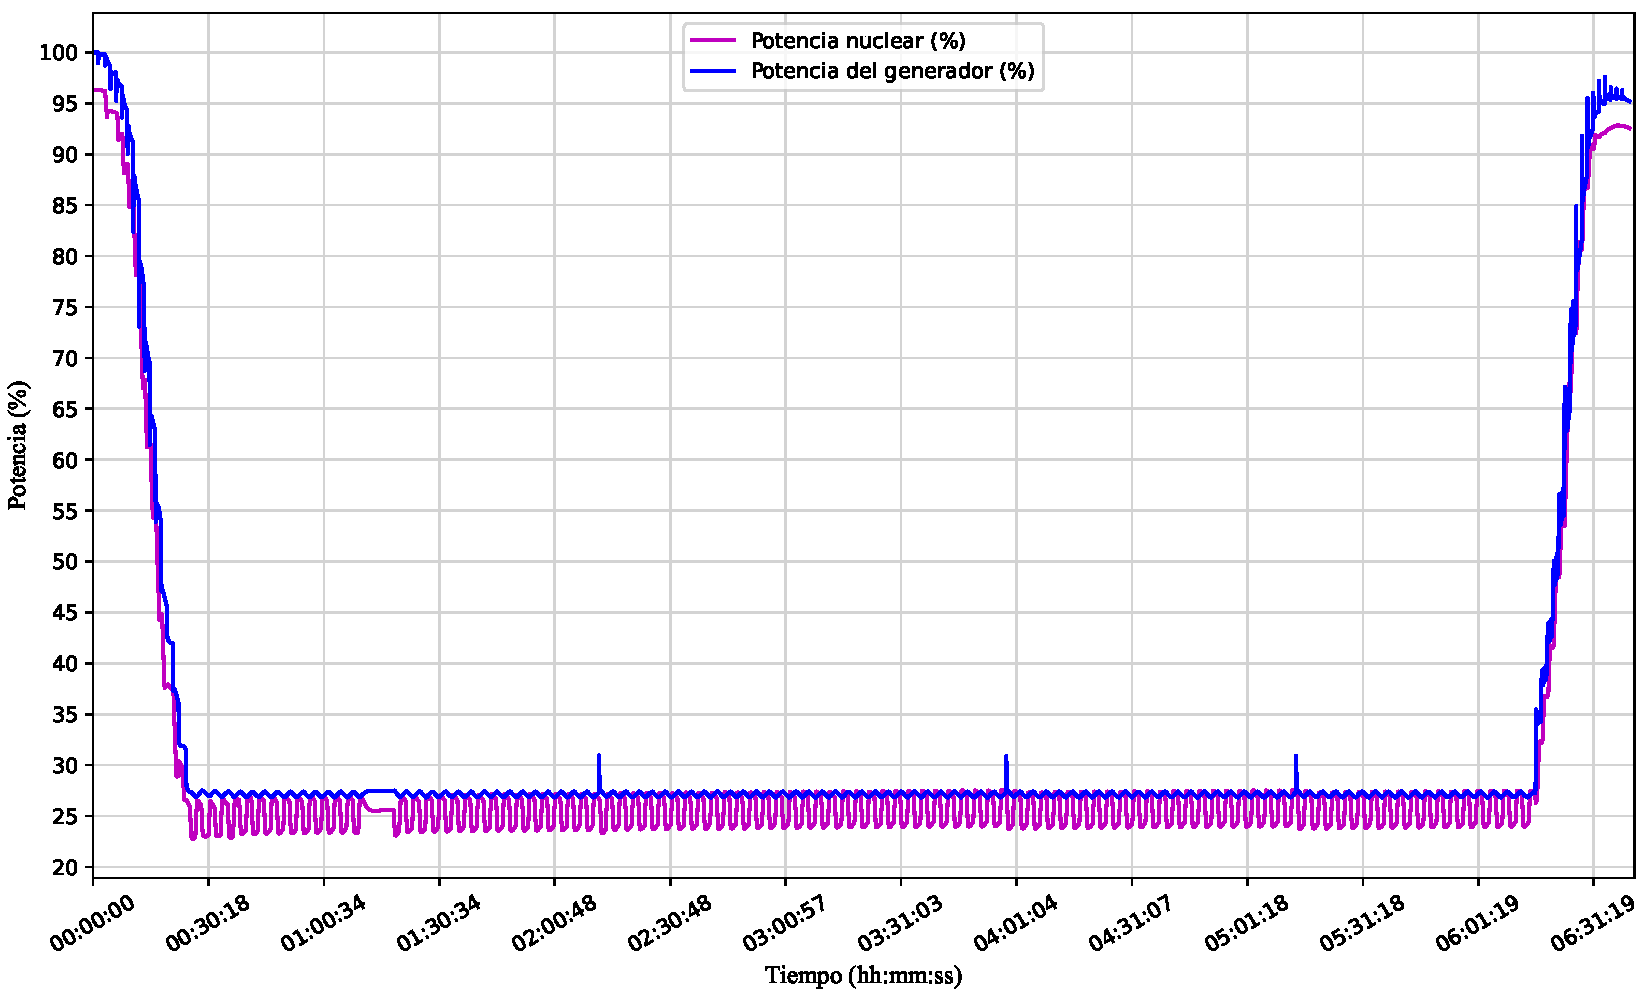
\includegraphics[width=\textwidth]{content/figures/sim2_potencias_arreglo.pdf}
      \vspace{-0.3cm}
      \caption{Variación de potencias en una maniobra de  seguimiento de carga (100 - 25 - 100\%) de 6 horas y 40 minutos realizada en el \acrshort{sgiz} simulando la adaptación a las horas de máxima producción solar de un día de invierno. Tasa de variación de carga empleada: 3\%/min.}
      \label{fig:sim2_potencias}
    \end{figure}
\end{enumerate}

\paragraph{Respuestas a las cuestiones planteadas} \label{respuestas_cuestiones_planteadas}

\textit{Simulación de 45 minutos realizada en el \acrshort{sgiz} el 12 de abril de 2024.}

A continuación se muestran las gráficas obtenidas en la simulación, junto con las respuestas a las cuestiones planteadas. El objetivo de las cuestiones es apoyar el análisis de las gráficas. 

\begin{figure}[!h]
  \centering
  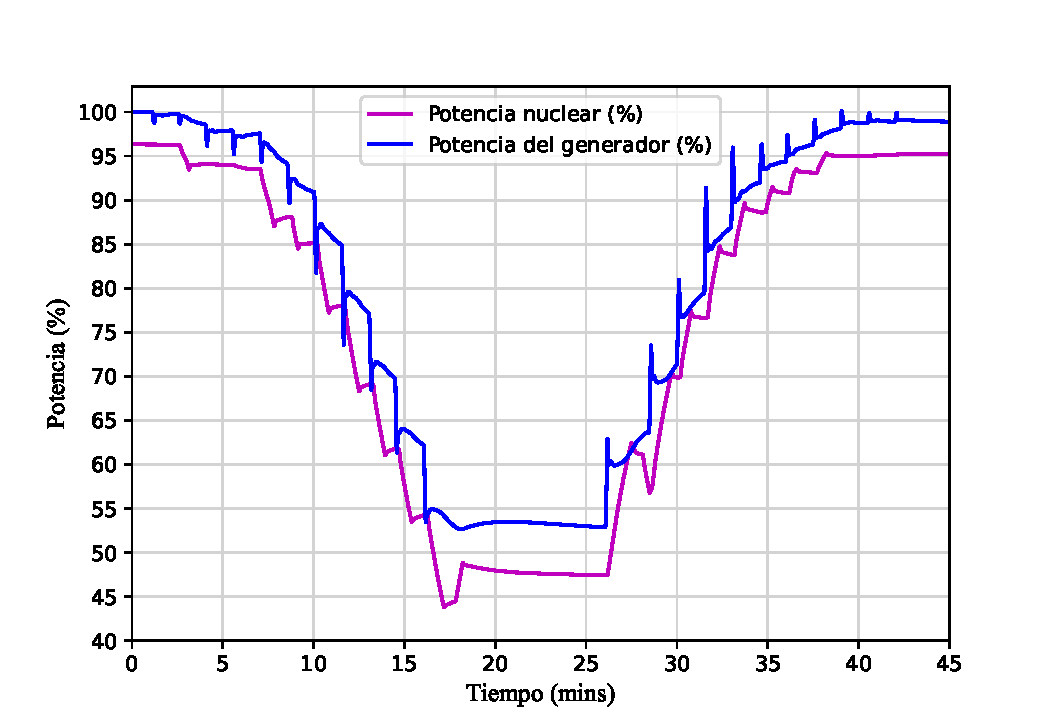
\includegraphics[width=0.75\textwidth]{content/figures/sim1_potencias.pdf}
  \caption{\textit{Gráfica 1} - Variaciones de potencia.}
  \label{fig:sim1_potencias}
\end{figure}

\begin{figure}[!h]
  \centering
  \vspace{-0.3cm}
  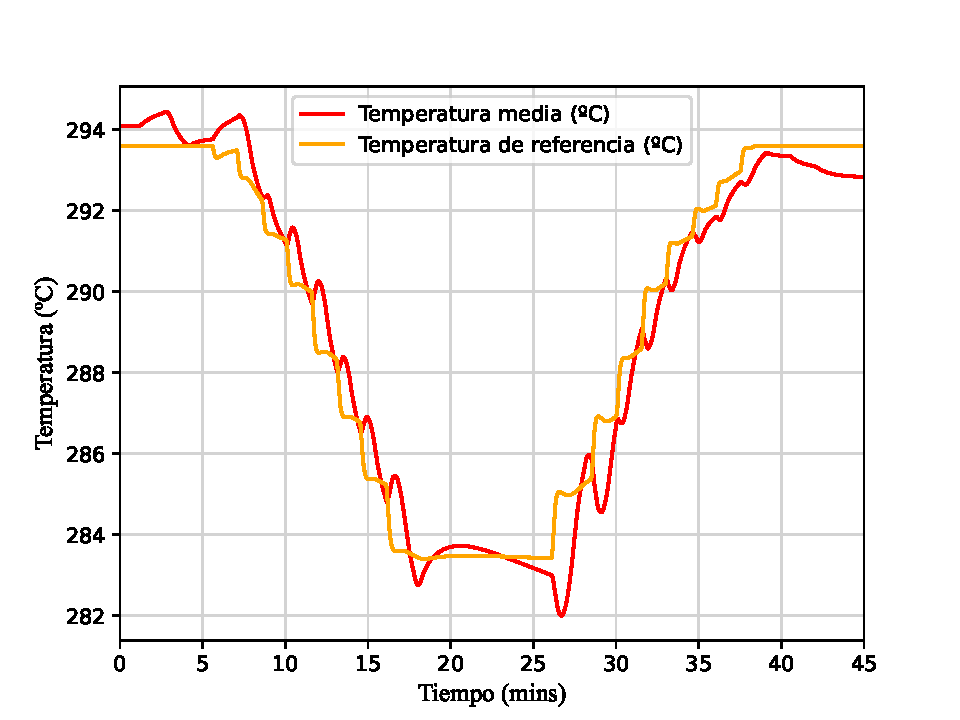
\includegraphics[width=0.62\textwidth]{content/figures/sim1_temperaturas.pdf}
  \vspace{-0.3cm}
  \caption{\textit{Gráfica 2} - Variaciones de temperatura.}
  \label{fig:sim1_temperaturas}
\end{figure}

\underline{Cuestión gráficas 1 y 2:} Al cerrar las válvulas de control de la turbina para disminuir la potencia, se reduce el gasto de vapor y el foco frío de la planta se hace menos eficiente. Esto provoca ``saturaciones'' en el circuito primario que originan picos de aumento de temperatura. Como el coeficiente de temperatura del moderador es negativo, estos aumentos de temperatura conllevan picos de disminución de la potencia. Cuando se aumenta la potencia en la turbina sucede lo contrario. Cabe destacar que estos picos se amplifican cuando trabajamos a potencias bajas ---en este caso, alrededor del 50\%--- ya que se trata de una zona de menor estabilidad para el sistema de control del reactor.

\underline{Observaciones adicionales:} En primer lugar, la \textit{gráfica 1} muestra perfectamente el comportamiento \textit{reactor sigue a turbina}. Primero disminuye la potencia de la turbia y, pasados unos instantes, disminuye la potencia nuclear, y así sucesivamente.

En segundo lugar, los picos de temperatura ocasionados por el cierre o apertura de las válvulas de regulación de la turbina se podrían amortiguar e, incluso, mitigar empleando la técnica de derivación del vapor sin pasar por la turbina. Este vapor ---al mismo tiempo que se lleva a cabo el seguimiento de carga--- podría emplearse para las aplicaciones de cogeneración detalladas en el apartado \ref{cogeneracion}.

\begin{figure}[!h]
  \centering
  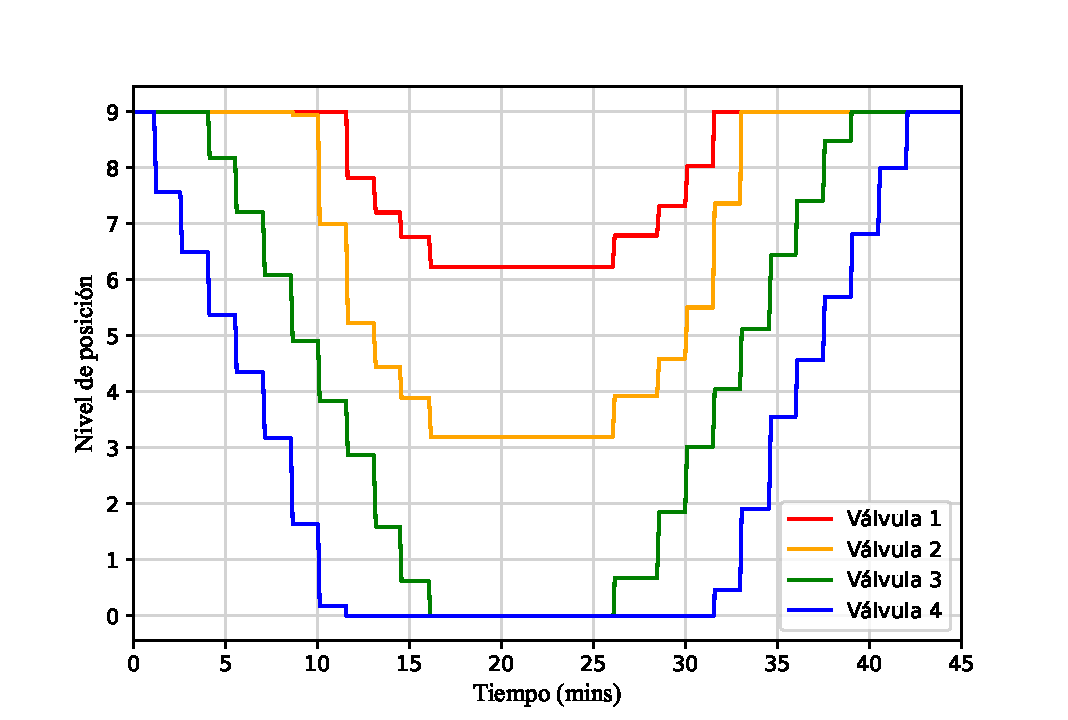
\includegraphics[width=0.63\textwidth]{content/figures/sim1_valvulas_control.pdf}
  \caption{\textit{Gráfica 3} - Posición de las válvulas de admisión de vapor a la turbina.}
  \label{fig:sim1_valvulas_control}
\end{figure}

\begin{figure}[h]
  \centering
  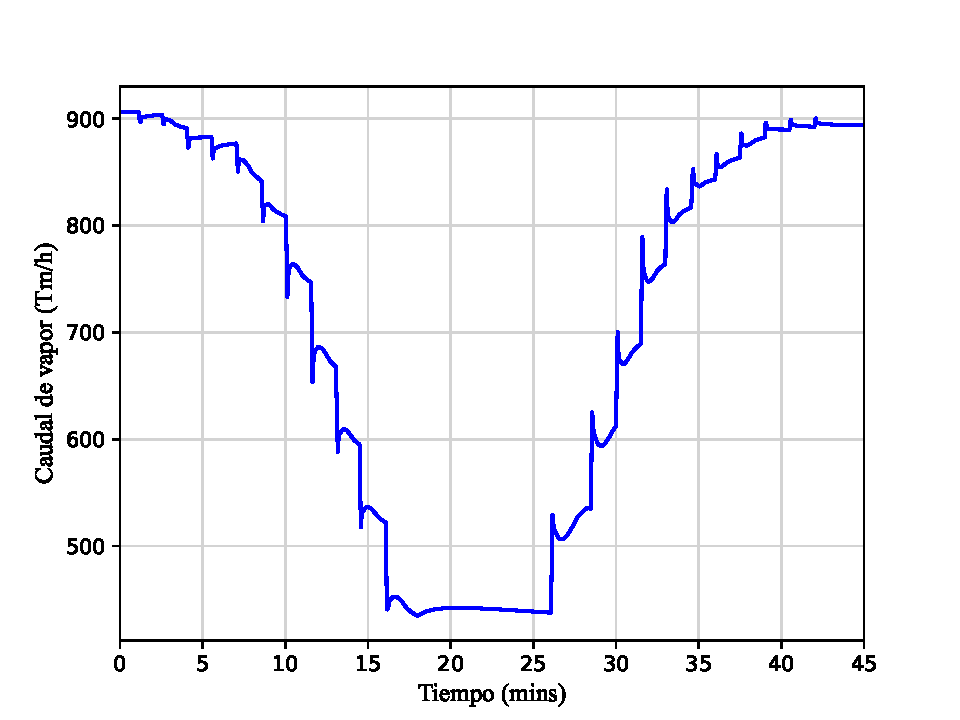
\includegraphics[width=0.67\textwidth]{content/figures/sim1_vapor.pdf}
  \caption{\textit{Gráfica 4} - Caudal de vapor que entra a la turbina.}
  \label{fig:sim1_vapor}
\end{figure}

\underline{Observaciones:} Al cerrar las válvulas de regulación, disminuye el caudal ---y, por tanto, el gasto másico--- de vapor que entra en la turbina. La gran influencia del caudal de vapor sobre la potencia generada por la turbina se pone de manifiesto al observar que el comportamiento de las curvas de \textit{caudal de vapor} y de \textit{potencia del generador} es idéntico.

\begin{figure}[!h]
  \centering
  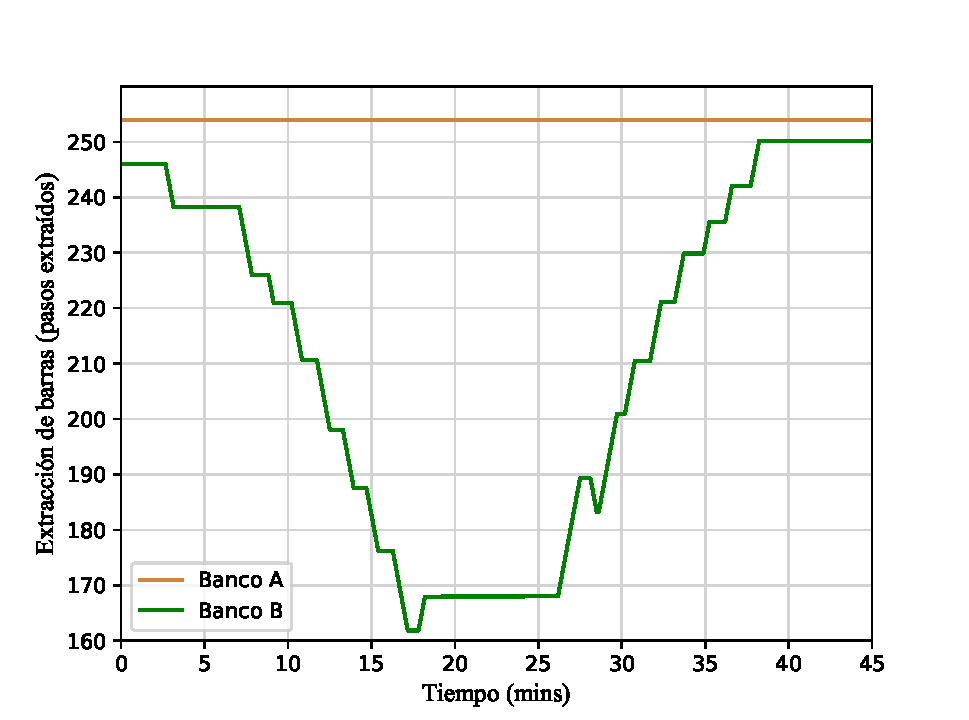
\includegraphics[width=0.62\textwidth]{content/figures/sim1_barras_control.pdf}
  \caption{\textit{Gráfica 5} - Inserción de las barras de control en el núcleo de reactor.}
  \label{fig:sim1_barras_control}
\end{figure}

\underline{Cuestión gráfica 5:} El sistema de control automático del reactor responde a las diferencias superiores a 0.83ºC entre la $T_{med}$ y la $T_{ref}$. Si la $T_{med}$ supera en 0,83ºC a la $T_{ref}$, se insertan las barras de control, insertando así reactividad negativa, pues el primario está dando una potencia mayor que la demandada por el secundario. En el caso contrario, se extraen las barras de control. De esta manera, se ajusta la temperatura real con la de referencia, ajustando al mismo tiempo la potencia nuclear con la nueva potencia demandada en la turbina.

\underline{Observación adicional:} Comparando esta curva de inserción de barras con la de la \textit{potencia nuclear}, se observa que tienen un comportamiento prácticamente idéntico, lo que refleja la rápida respuesta del sistema automático de inserción de barras de control.

\begin{figure}[h]
  \centering
  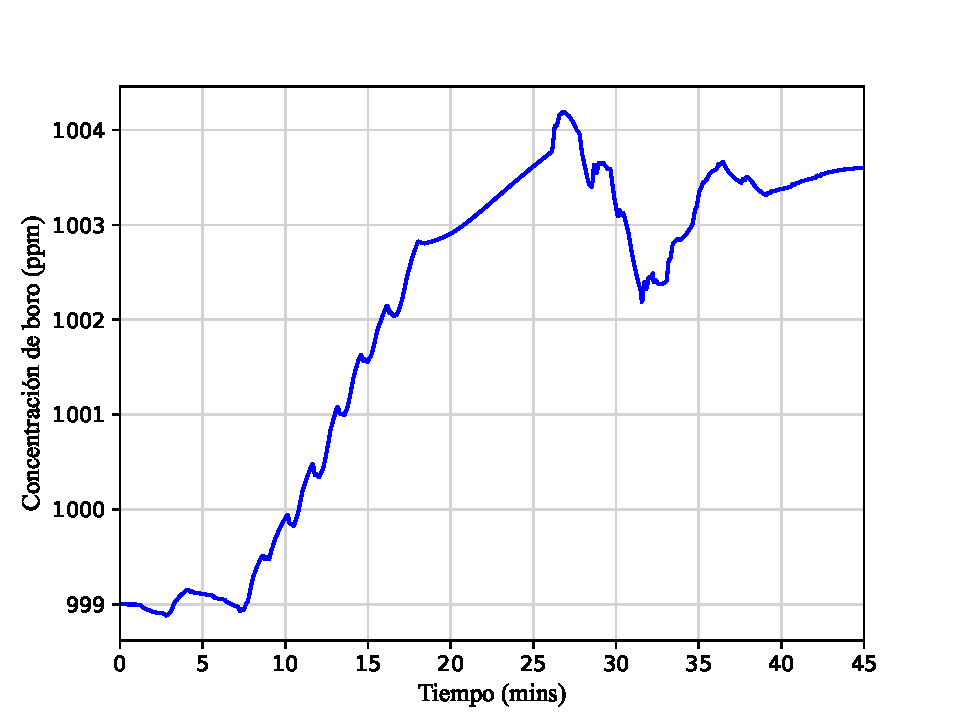
\includegraphics[width=0.75\textwidth]{content/figures/sim1_boro.pdf}
  \caption{\textit{Gráfica 6} - Variación en la concentración de boro en el circuito primario.}
  \label{fig:sim1_boro}
\end{figure}

\underline{Cuestión gráfica 6:} La inserción de barras de  control es muy efectiva, pero provoca una distorsión en la distribución del flujo neutrónico y, por tanto, de la potencia, ya que se agota más el combustible en la parte inferior del reactor que en la parte superior, por donde se insertan dichas barras en el caso de los \acrshortpl{pwr}. La inyección de ácido bórico es especialmente interesante para compensar estos desequilibrios en la distribución del flujo a lo largo del núcleo del reactor.

\underline{Observación adicional:} La curva demuestra el lento aumento en la concentración de boro cuando así se requiere, pues tarda una cantidad considerable de tiempo en aumentar muy ligeramente su concentración.

\begin{figure}[!h]
  \centering
  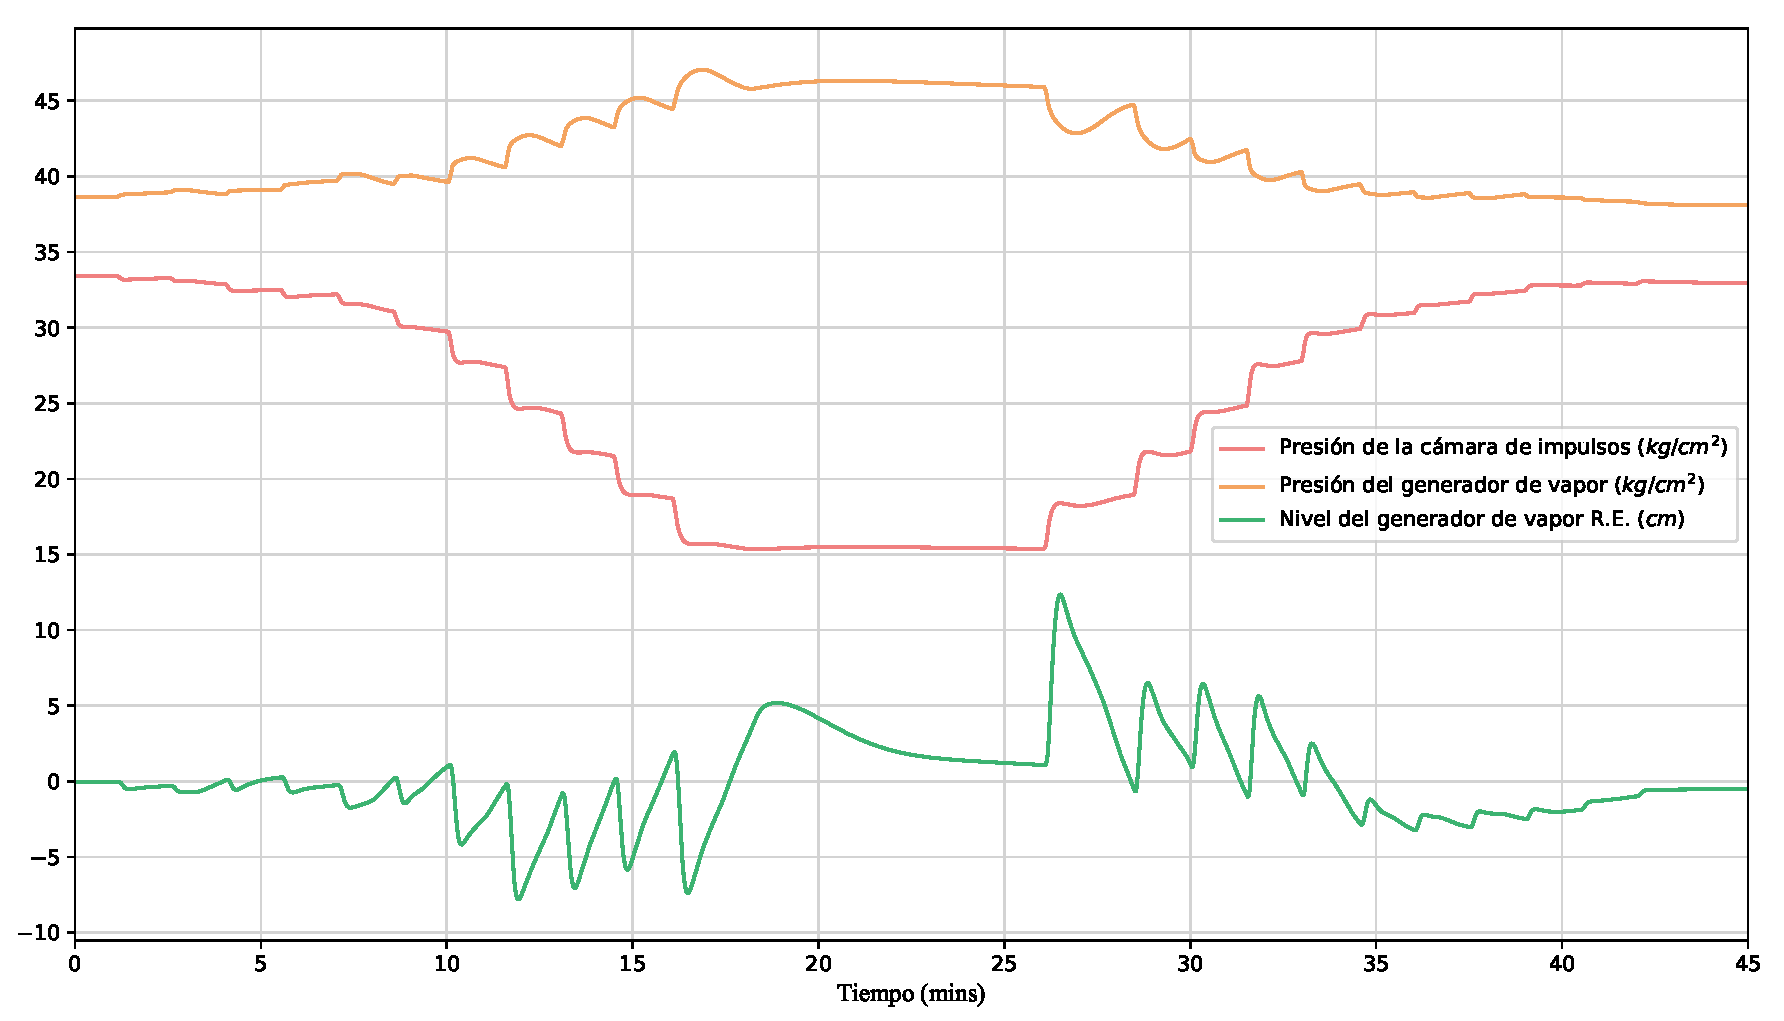
\includegraphics[width=\textwidth]{content/figures/sim1_gen_vapor_camara_imp.pdf}
  \caption{\textit{Gráfica 7} - Propiedades del generador de vapor y la cámara de impulsos.}
  \label{fig:sim1_gen_vapor_camara_imp}
\end{figure}

\begin{figure}[!h]
  \centering
  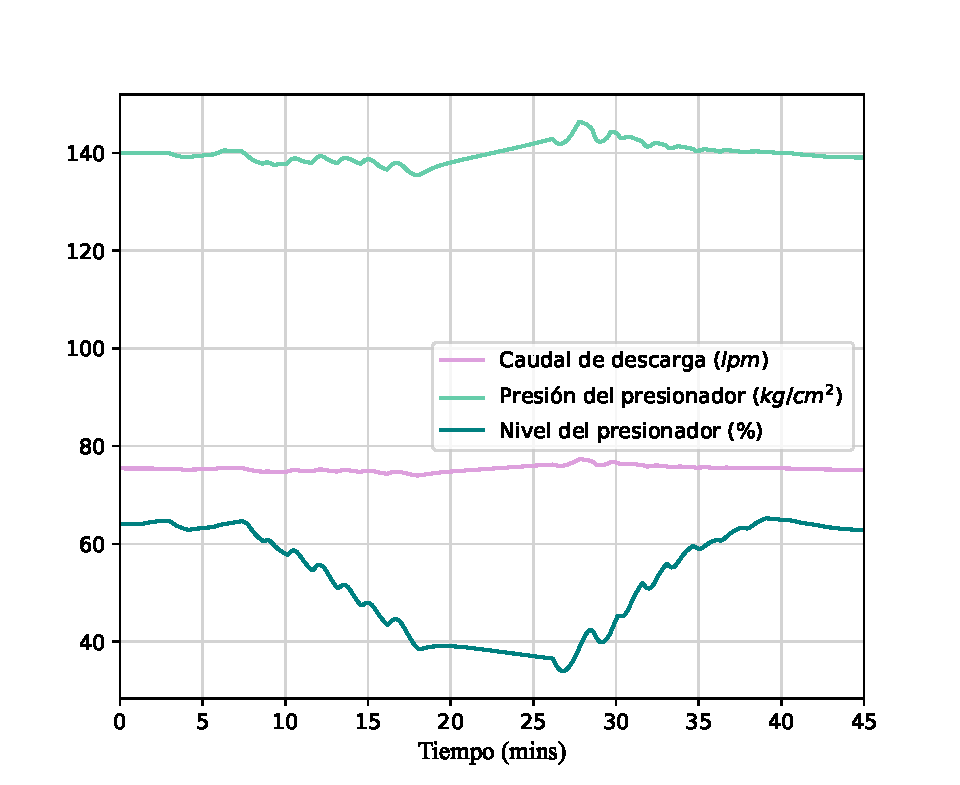
\includegraphics[width=0.7\textwidth]{content/figures/sim1_presionador.pdf}
  \caption{\textit{Gráfica 8} - Propiedades del presionador.}
  \label{fig:sim1_presionador}
\end{figure}

\underline{Cuestión gráficas 7 y 8:} Al ser esta una cuestión más amplia, se aprovecha para explicar el comportamiento general del sistema, justificando así las tendencias de las \textit{gráficas 7 y 8}. Sin embargo, no es necesario que la explicación del alumno sea de esta extensión.

Al cerrar parcialmente las válvulas de admisión de vapor a la turbina de alta presión, a parte de disminuir el gasto de vapor entrante a la turbina, el vapor sufre un proceso de laminación, disminuyendo su presión en el interior de la cámara de impulsos\footnote{Es la cámara de admisión de vapor al primer escalonamiento de la turbina.} ---tal y como se muestra en la curva roja de la \textit{gráfica 7}---. De esta manera, disminuye el salto entálpico y, por tanto, la potencia generada por la turbina. Al disminuir la potencia, disminuye la ($T_{ref}$) asociada al secundario.

Asimismo, al disminuir el gasto de vapor entrante a la turbina, como inmediatamente no se ha actuado sobre ningún otro componente, en el generador de vapor se sigue produciendo la misma cantidad de vapor, lo que provoca una acumulación o ``saturación'' del mismo hasta las válvulas de entrada a la turbina, aumentando así la presión en la admisión (aguas arriba de las válvulas) y en el generador de vapor ---tal y como se muestra en la curva naranja de la \textit{gráfica 7}---. Al ser el generador de vapor un sistema en equilibrio líquido-vapor, el incremento de presión conlleva un incremento de temperatura.

Al detectarse variaciones cada vez más grandes en el nivel del generador de vapor ---tal y como se aprecia en la curva verde de la \textit{gráfica 7}---, el sistema de control del nivel ordena el cierre de válvula de entrada al generador de vapor (válvula LCV-1947), disminuyendo el caudal de agua de alimentación. De esta manera, se consigue estabilizar la presión del generador de vapor, aunque siga siendo mayor a la nominal. 

Como consecuencia del calentamiento del circuito secundario y la reducción del caudal de agua de alimentación, la refrigeración del primario es menos efectiva, lo que provoca un aumento de la $T_{med}$ del primario. Tal y como se ha comentado anteriormente, al superar en 0.83ºC la $T_{ref}$, el sistema de control inserta automáticamente las barras de control, disminuyendo así la $T_{med}$ y la potencia del reactor. Estas subidas y bajadas de la $T_{med}$ del primario, provocan oscilaciones en la presión y en el nivel del presionador, así como en el caudal de descarga ---tal y como se observa en la \textit{gráfica 8}---:

\begin{itemize}
  \item En las fases de aumento de la $T_{med}$, aumenta consecuentemente la presión en el presionador. Asimismo, el agua se dilata y sube el nivel del presionador. El control de nivel del presionador ordena automáticamente al sistema de control volumétrico que aumente el caudal de descarga con el fin de disminuir dicho nivel al nuevo valor fijado por la $T_{med}$. 
  \item En las fases de disminución de la $T_{med}$ por el avance en la inserción de las barras de control, ocurre lo contrario: al disminuir la presión del presionador, el agua se contrae y es necesario disminuir el caudal de descarga.
\end{itemize}

Estos aumentos y disminuciones de la presión del presionador pueden provocar la actuación automática de la ducha principal (válvula PCV-400A) y de los calentadores, respectivamente.

Por último, es importante remarcar que el análisis realizado para responder a esta cuestión se ha hecho para el caso de la bajada de carga, pero todos los fenómenos descritos ocurren exactamente al revés cuando se produce una subida de potencia, tal y como se observa en las gráficas obtenidas.

\underline{Tabla de resultados y cuestión SMRs}: Tal y como se ha comentado en el \textit{procedimiento} de la simulación (apartado \ref{procedimiento}), la Central Nuclear de Zorita permite una correcta adaptación automática a variaciones de potencia entre el 15 y el 100\% cuando se emplean tasas de variación de carga de alrededor del 3\%/min, permitiendo llevar a cabo una maniobra considerablemente rápida de seguimiento de carga. Los valores obtenidos en la \textit{tabla de resultados} (tabla \ref{tab:resultados_simulacion1_solucion}) y las curvas de potencia de la \textit{gráfica de la simulación de larga duración} (figura \ref{fig:sim2_potencias}) lo demuestran. De hecho, en esta última gráfica obtenida en el \acrshort{sgiz} (figura \ref{fig:sim2_potencias}), se observa una maniobra de seguimiento de carga análoga ---pero con mayores tasas de variación de potencia--- a la gráfica obtenida en un estudio real sobre el seguimiento de carga con \acrlongpl{smr} (figura \ref{fig:seguimiento de carga_smr}). Además, tal y como se observa en la tabla de \textit{capacidad de seguimiento de carga de los \acrshortpl{smr}} (tabla \ref{tab:capacidad_seguimiento_de_carga_smrs}), los \acrshortpl{smr} de tipo \acrshort{pwr} tienen aproximadamente el mismo rango permitido y las mismas rampas de potencia, por lo que se puede decir que el \acrshort{sgiz} permite realizar una aproximación realista de lo que sería una operación de seguimiento de carga en un \acrshort{smr} de tipo \acrshort{pwr}, como lo es el AP300, por ejemplo. Aun así, es importante destacar que, a diferencia de las centrales nucleares convencionales ---o de la misma central de José Cabrera---, destinadas principalmente a operar como centrales base, los \acrshortpl{smr} se diseñan con el objetivo de facilitar la adaptación a redes eléctricas con fuertes penetraciones de energías renovables intermitentes. Por tanto, una maniobra de seguimiento de carga como esta supone forzar considerablemente la central nuclear en cuestión ---tal y como demuestran las inestabilidades de la gráfica \ref{fig:sim2_potencias} a potencias muy bajas---, mientras que los pequeños reactores modulares se conciben para realizar a menudo esta operación sin que ello suponga ninguna desestabilización del sistema ni ningún daño para sus equipos.

\begin{table}[h]
  \centering
  \resizebox{1\textwidth}{!}{%
  \begin{tabular}{|c|c|c|c|c|c|c|}
    \hline
    \rowcolor[HTML]{ECF4FF} 
    \textbf{\begin{tabular}[c]{@{}c@{}}Potencia inicial\\ (MWe \\ generados\\  y \% nuclear)\end{tabular}} &
      \textbf{\begin{tabular}[c]{@{}c@{}}Potencia \\ intermedia\\ (MWe generados\\  y \% nuclear)\end{tabular}} &
      \textbf{\begin{tabular}[c]{@{}c@{}}Duración \\ bajada\\ de potencia\\ (min)\end{tabular}} &
      \textbf{\begin{tabular}[c]{@{}c@{}}Rampa media\\ de potencia \\ en la bajada\\ (\%/min)\end{tabular}} &
      \textbf{\begin{tabular}[c]{@{}c@{}}Potencia final\\ (MWe \\ generados\\  y \% nuclear)\end{tabular}} &
      \textbf{\begin{tabular}[c]{@{}c@{}}Duración \\ subida\\ de potencia \\ (min)\end{tabular}} &
      \textbf{\begin{tabular}[c]{@{}c@{}}Rampa media \\ de potencia\\ en la subida \\ (\%/min)\end{tabular}} \\ \hline
    \cellcolor[HTML]{FFFFFF}\begin{tabular}[c]{@{}c@{}}142,65 MWe\\ 96,3\%\tablefootnote{Por un error de diseño en la Central Nuclear de Zorita, el 100\% de turbina corresponde al 96,3\% de potencia del reactor.} nuclear\end{tabular} &
      \begin{tabular}[c]{@{}c@{}}75,5 MWe\\ 47,5\% nuclear\end{tabular} &
      16,5 mins &
      2,96 \%/min &
      \begin{tabular}[c]{@{}c@{}}141,1 MWe\\ 95,3\% nuclear\end{tabular} &
      19 mins &
      2,52 \%/min \\ \hline
    \end{tabular}
  }
  \caption{Resultados de la maniobra corta de seguimiento de carga realizada en el \acrshort{sgiz}.}
  \label{tab:resultados_simulacion1_solucion}
  \end{table}

\subsubsection{\textit{Feedback} de la práctica} \label{feedback_practica}

La implementación de la simulación anterior como práctica de la asignatura de \textit{Tecnologías Avanzadas en Reactores Nucleares} tuvo lugar por primera vez el jueves 23 de mayo de 2024. Se llevó a cabo en dos turnos de 2 horas y de 14 alumnos de máster cada uno. Las explicaciones de la misma fueron realizadas por el técnico de laboratorio encargado del \acrshort{sgiz} y por el autor del presente proyecto.

Al tratarse de una práctica nueva, se envió tras su finalización un formulario a todos los alumnos asistentes para que proporcionaran el \textit{feedback} necesario. Todos los resultados detallados de la encuesta se muestran en el anexo \ref{resultados_encuesta_practica}. En resumen, el grado de satisfacción general con la práctica realizada fue elevado, tal y como se muestra en la figura \ref{fig:encuesta_8_memoria}. La simulación realizada ---junto con las explicaciones correspondientes--- ayudó a los alumnos a comprender mejor las características y el funcionamiento general de los principales componentes y sistemas del reactor durante la operación del mismo. Asimismo, permitió profundizar en una característica importante de los \acrshortpl{smr}: el seguimiento de carga. 

Un aspecto a mejorar en el que coincidieron todos los alumnos fue la fecha de realización de la misma. Al ser a finales de curso, se juntó con entregas de trabajos y exámenes, por lo que para próximas ocasiones debería realizarse antes, óptimamente justo después de ver los \acrshortpl{smr}. Por otro lado, algunos comentaron que la práctica se centraba en un aspecto muy concreto de uno de los temas estudiados en la asignatura, por lo que no tenía una gran relación con la asignatura en su conjunto. Propusieron que podría reestructurarse en cuanto al contenido para que se trabajase un abanico más amplio de características de los reactores avanzados. Además, les pareció una práctica muy interesante para implementarse en la asignatura de 4º de grado de \textit{Centrales Nucleares}.

Por último, manifestaron un contento común en lo referente a la realización de sesiones prácticas en el \acrshort{sgiz}, ya que ayuda a ver y aplicar de primera mano los conceptos explicados de forma teórica en el aula. \textit{``Toda actividad que sea salir de las clases y de la teoría, ayuda a entender mejor las cosas''}, afirmó un alumno. A continuación, se muestra el resultado de una pregunta en la que se pedía una valoración numérica sobre el desarrollo general de la práctica:

\begin{itemize}
  \item \underline{Pregunta 8 de la encuesta:} \textbf{Valora del 0 al 10 tu grado de satisfacción general con la práctica realizada:}
\end{itemize}
   
    \begin{figure}[!h]
        \centering
        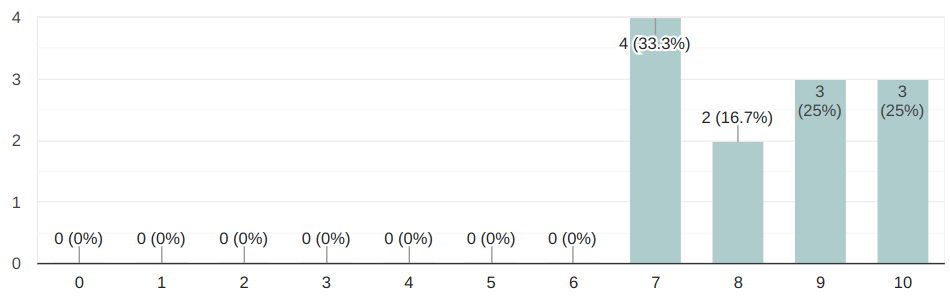
\includegraphics[width=\textwidth]{content/figures/encuesta_8.png}
        \caption{Valoración de la satisfacción general de los alumnos con la práctica realizada (ver el resto de respuestas en el anexo \ref{resultados_encuesta_practica}).}
        \label{fig:encuesta_8_memoria}
    \end{figure}


\newpage
\subsection{Simulaciones largas de seguimiento de carga fallidas}

El interés que presenta simular maniobras de seguimiento de carga más largas es que se puede imitar un escenario realista de adaptación a las renovables o a la curva de demanda eléctrica, además de que permite observar los efectos del xenón ante las variaciones de potencia.

\subsubsection{Primera simulación larga fallida}

La primera simulación que se ha intentado realizar es una maniobra de variación de potencia 100 - 20 - 100\% de unas 7 horas de duración. Debido a que el \acrshort{sgiz} casi siempre se ha empleado en el modo de ejecución a tiempo real, se ha considerado inicialmente que la mejor opción es realizar la simulación en el modo de ejecución a tiempo real sin alarmas, ya que el simulador se puede dejar funcionando solo largas horas y es mejor evitar el ruido de las alarmas.

Tras las 7 horas de simulación, se ha procedido a la obtención de las gráficas de tendencias. Sin embargo, estas gráficas son incorrectas y proporcionan un comportamiento y unos valores que no se corresponden en absoluto con la simulación. Tras intentar averiguar la causa del fallo en vano, se ha tenido que cerrar la simulación sin poder obtener los resultados de la misma.

\paragraph{Lecciones aprendidas}

\begin{itemize}
  \item El simulador permite la graficación a tiempo real de los parámetros de interés a medida que avanza la simulación. Es importante comenzar esta graficación desde el primer momento para asegurarse que los resultados se están guardando y graficando correctamente.
  \item El modo de ejecución a tiempo real sin alarmas puede fallar ---o por lo menos ha fallado en esta ocasión--- a la hora de proporcionar los resultados.
\end{itemize}

\subsubsection{Segunda simulación larga fallida} \label{sim_larga_fallida}

Ante el fallo en la anterior experiencia, se ha procedido a realizar la misma simulación pero en el modo de ejecución a tiempo real con alarmas activadas.

En este caso, la simulación se ha podido llevar a cabo con normalidad y las gráficas se han generado correctamente. Sin embargo, como la simulación se ha dejado correr sin ser supervisada durante algunos periodos de tiempo, cuando esta llevaba 6 horas, se ha observado que la graficación se ha detenido a las 4 horas, mientras que la simulación seguía avanzando. Tras intentar averiguar en vano la causa del fallo y el modo de solucionarlo, se ha decidido grabar aquel instante de la simulación como condición inicial. De esta manera, se puede reiniciar el simulador, cargar la condición inicial guardada y seguir desde el punto en el que se ha dejado anteriormente. Sin embargo, esta condición inicial se ha cargado con los valores de todas las variables en el instante en el que se ha grabado la condición, pero sin tener en cuenta el comportamiento oscilatorio que presentaba el reactor en ese momento al encontrarse a tan bajas potencias (alrededor del 20\%). Por eso, las gráficas obtenidas presentan un cambio de comportamiento ---una estabilización--- que no se corresponde con el comportamiento real de dichas variables (ver \textit{Anexo} \ref{graficas_erroneas}).

\paragraph{Lección aprendida}

\begin{itemize}
  \item El modo de ejecución a tiempo real con alarmas activadas tiene programado un periodo máximo de graficación de 4 horas, fallo que ha sido notificado a la empresa desarrolladora.
\end{itemize}

\newpage
\subsection{Simulaciones largas de seguimiento de carga exitosas}

Ante las anteriores simulaciones fallidas, se ha decidido probar el modo de ejecución rápido (FAST) sin alarmas, por el considerable ahorro de tiempo que conlleva (velocidad $\times 20$) y para probar si ---por casualidad--- ofrece la posibilidad de graficar más allá de 4 horas. Tras realizar unas pruebas, se ha comprobado que, efectivamente, el modo FAST funciona correctamente y permite la graficación de simulaciones de larga duración. Con esto, se han realizado bastante rápido las siguientes simulaciones, que representan dos casos reales distintos ---y muy habituales--- de seguimiento de carga. El procedimiento es análogo al explicado en el punto \ref{procedimiento}.

\subsubsection{Adaptación a la generación solar}

\textit{Simulación de 9 horas y 45 minutos realizada en el \acrshort{sgiz} el 17 de junio de 2024.}

\paragraph{Contextualización}

La curva de generación solar durante un día soleado es como se muestra a continuación:

\begin{figure}[!h]
  \centering
  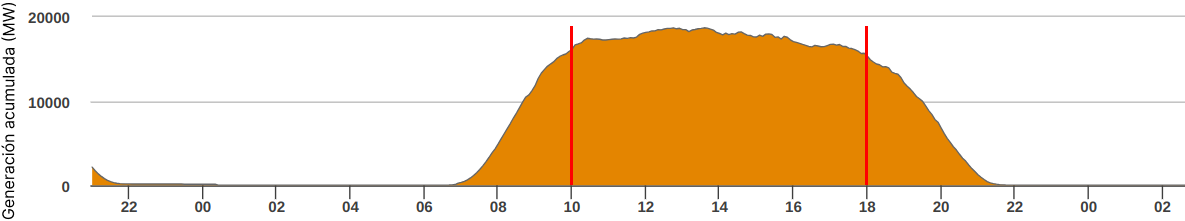
\includegraphics[width=0.95\textwidth]{content/figures/generacion_solar.png}
  \caption{Generación solar en España durante el 17 de junio de 2024, donde la máxima producción se da aproximadamente durante 8 horas: entre las 10.00 y las 18.00 (\cite{ree_demanda}).}
  \label{fig:generacion_solar}
\end{figure}

En estos casos, especialmente cuando también hay un fuerte apoyo de la eólica, resulta interesante poder realizar seguimiento de carga para adaptarse a las horas de máxima producción solar. Esta disminución de la potencia nuclear y mantenimiento de la misma al 20\% durante las 8 horas de máxima producción solar, es la que se pretende realizar en esta simulación.

\paragraph{Análisis de los resultados}

A continuación, se procede al análisis detallado de las gráficas obtenidas, el cual permite comprender el comportamiento del reactor en el transcurso de la maniobra realizada.

En primer lugar, las figuras \ref{fig:sim3_potencias} y \ref{fig:sim3_temperaturas} muestran las curvas de las variaciones de potencia y de temperatura, respectivamente. De ellas se extrae la siguiente información:

\begin{itemize}
  \item La figura \ref{fig:sim3_potencias} muestra claramente el comportamiento \textit{reactor sigue a turbina}. Primero disminuye la potencia de la turbina al ir cerrando las válvulas de control, pasados unos instantes, disminuye la potencia nuclear, y así sucesivamente.
  \item Tanto en la bajada como en la subida de potencia se observan en las curvas de potencia y de temperatura los picos característicos en este tipo de maniobras. Tal y como se explica en el apartado \ref{respuestas_cuestiones_planteadas} de la simulación corta, al cerrar las válvulas de control de la turbina para disminuir la potencia, se reduce el gasto de vapor y el foco frío de la planta se hace menos eficiente. Esto provoca “saturaciones” en el circuito primario que originan picos de aumento de temperatura (figura \ref{fig:sim3_temperaturas}). Como el coeficiente de temperatura del moderador es negativo, estos aumentos de temperatura originan picos de disminución de la potencia (figura \ref{fig:sim3_potencias}). Cuando se abren las válvulas de control de la turbina para aumentar la potencia, sucede totalmente lo contrario.
  \item Las oscilaciones de las curvas cuando el reactor se encuentra a muy baja potencia, demuestran la inestabilidad de los reguladores PID del sistema de control automático del reactor en dichas condiciones. Esta inestabilidad se debe a que los reactores convencionales como Zorita estaban diseñados para operar fundamentalmente a potencia nominal.
  \item La diferencia entre los valores finales de potencia (cuando, en principio, se ha subido hasta la máxima potencia permitida en la turbina) y los valores iniciales antes de la bajada, se debe a que se trata de dos puntos con condiciones ---concentración de boro, concentraciones de xenón, nivel de extracción de las barras de control, etc.--- distintas. Entre ambos puntos han habido múltiples procesos y cambios en relación con el núcleo. Básicamente, al final de la simulación el intento de compensar las reactividades positivas y negativas resulta en una potencia inferior a la inicial fruto de una reactividad global negativa.
  \item Cabe destacar que, tal y como se muestra en la figura \ref{fig:sim3_temperaturas}, a partir de las 8 horas y 56 minutos de simulación, se da una gran divergencia final entre la temperatura media del primario y la temperatura de referencia. Tras intentar averiguar el posible sentido de este comportamiento, se concluye que probablemente en ese instante se ha producido un error de simulación, ya que las diferencias entre $T_{med}$ y $T_{ref}$ muy superiores a 2ºC conllevan la activación del \acrfull{sis}, el cual implica el disparo del reactor, cosa que no ha sucedido en la simulación. 
  \item Por último, se detallan a continuación las tasas de variación de potencia de la maniobra:
  
  \begin{table}[h]
    \centering
    \resizebox{1\textwidth}{!}{%
    \begin{tabular}{|c|c|c|c|c|c|c|}
      \hline
      \rowcolor[HTML]{ECF4FF} 
      \textbf{\begin{tabular}[c]{@{}c@{}}Potencia inicial\\ (MWe \\ generados\\  y \% nuclear)\end{tabular}} &
        \textbf{\begin{tabular}[c]{@{}c@{}}Potencia \\ intermedia\\ (MWe generados\\  y \% nuclear)\end{tabular}} &
        \textbf{\begin{tabular}[c]{@{}c@{}}Duración \\ bajada\\ de potencia\\ (min)\end{tabular}} &
        \textbf{\begin{tabular}[c]{@{}c@{}}Rampa media\\ de potencia \\ en la bajada\\ (\%/min)\end{tabular}} &
        \textbf{\begin{tabular}[c]{@{}c@{}}Potencia final\\ (MWe \\ generados\\  y \% nuclear)\end{tabular}} &
        \textbf{\begin{tabular}[c]{@{}c@{}}Duración \\ subida\\ de potencia \\ (min)\end{tabular}} &
        \textbf{\begin{tabular}[c]{@{}c@{}}Rampa media \\ de potencia\\ en la subida \\ (\%/min)\end{tabular}} \\ \hline
      \cellcolor[HTML]{FFFFFF}\begin{tabular}[c]{@{}c@{}}142,65 MWe\\ 96,3\% nuclear\end{tabular} &
        \begin{tabular}[c]{@{}c@{}}27,4 MWe\\ $\approx 22\%$ nuclear\end{tabular} &
        36 mins &
        2,05 \%/min &
        \begin{tabular}[c]{@{}c@{}}125,4 MWe\\ 86,6\% nuclear\end{tabular} &
        25 mins &
        2,58 \%/min \\ \hline
      \end{tabular}
    }
    \caption{Resultados de la maniobra de adaptación a la generación solar realizada en el \acrshort{sgiz}.}
    \label{tab:resultados_simulacion3}
    \end{table}

\end{itemize}

\begin{figure}[!h]
  \vspace{-0.7cm}
  \centering
  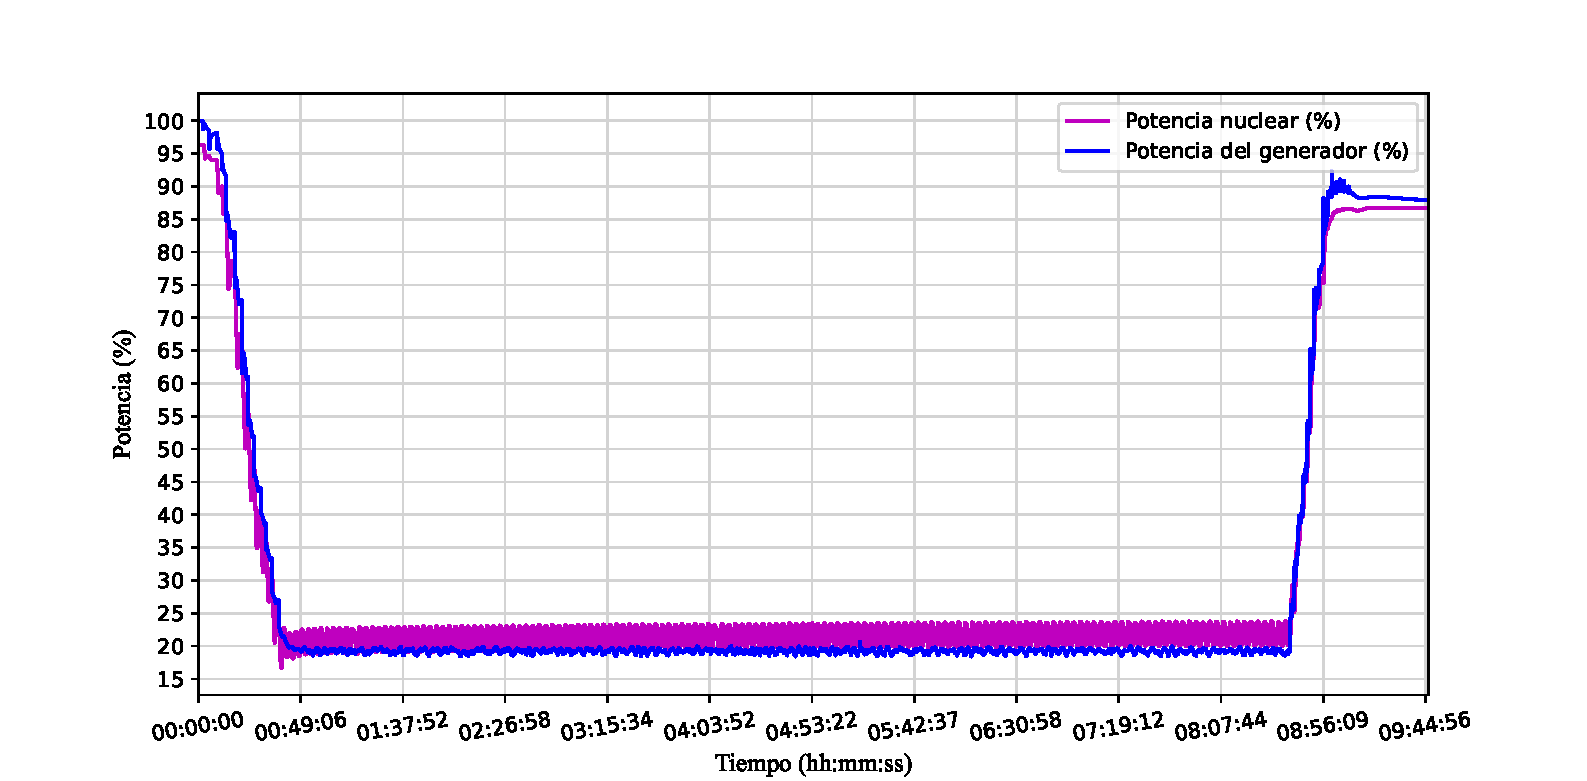
\includegraphics[width=0.95\textwidth]{content/figures/sim3_potencias.pdf}
  \caption{Variaciones de potencia en la simulación de adaptación a la generación solar.}
  \label{fig:sim3_potencias}
\end{figure}

\begin{figure}[!h]
  \vspace{-0.2cm}
  \centering
  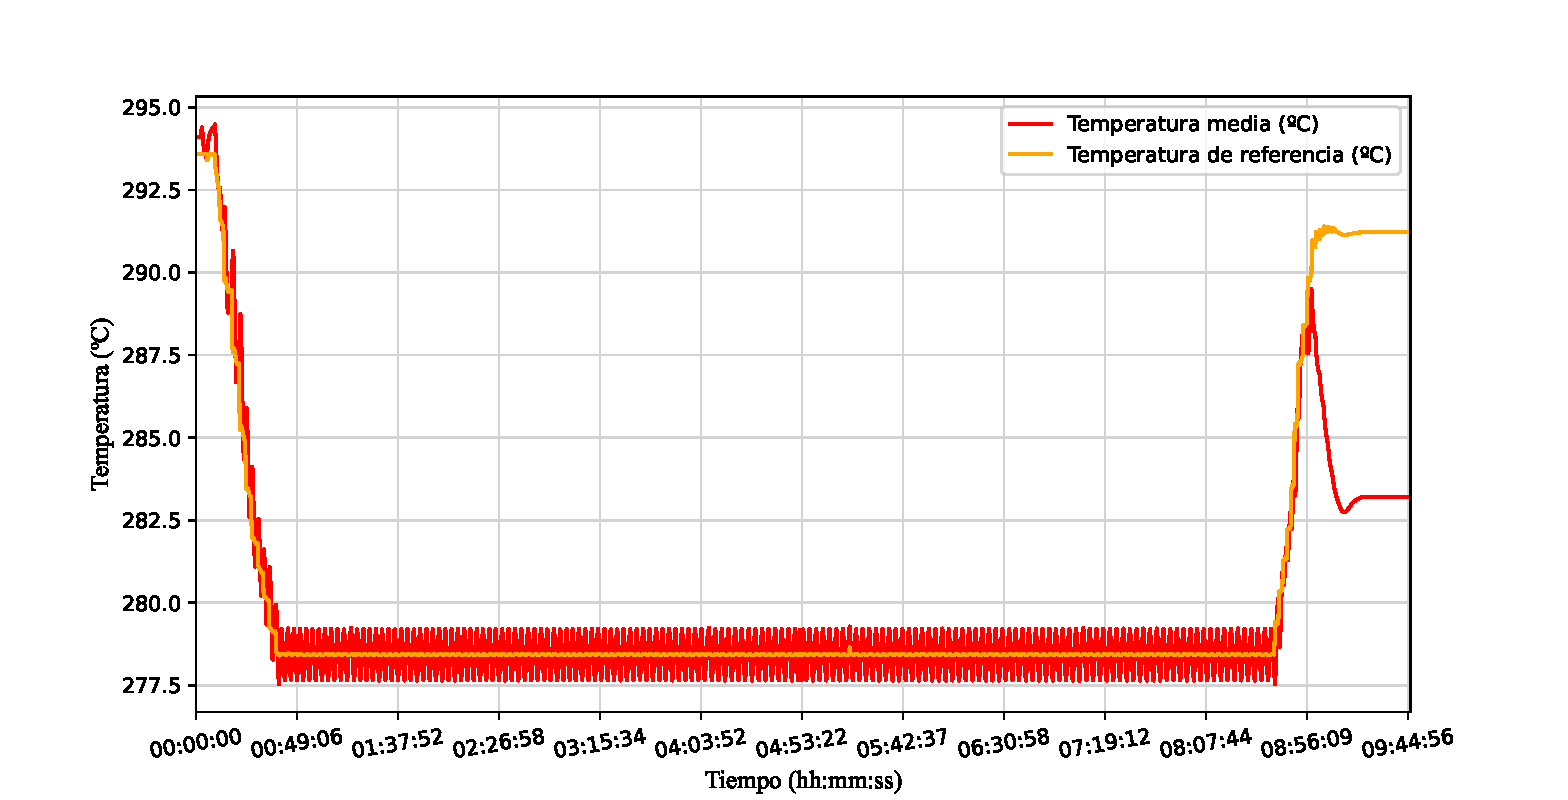
\includegraphics[width=\textwidth]{content/figures/sim3_temperaturas.pdf}
  \caption{Variaciones de temperatura en la simulación de adaptación a la generación solar.}
  \label{fig:sim3_temperaturas}
\end{figure}

En segundo lugar, la figura \ref{fig:sim3_valvulas_vapor} muestra las curvas de las válvulas de control de la turbina y la curva del caudal de vapor. El nivel de posición 9 de las válvulas de control corresponde al estado de apertura total y el nivel 0 al estado de cierre total, por lo que en esta maniobra solo llegan a cerrarse completamente las válvulas de admisión 3 y 4. Como es lógico, al cerrar las válvulas de regulación, disminuye el caudal ---y, por tanto, el gasto másico--- de vapor que entra en la turbina. Al mismo tiempo, se observa ---como es de esperar--- que el comportamiento de la curva del caudal de vapor es exactamente análogo al de la potencia eléctrica del generador acoplado a la turbina.

\begin{figure}[h]
  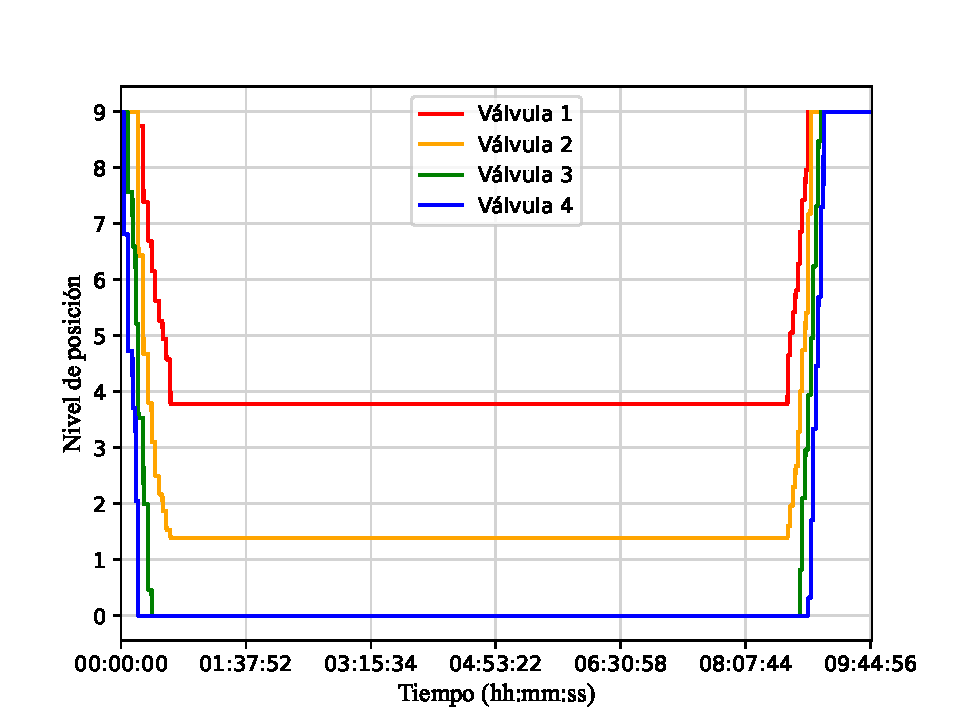
\includegraphics[width=0.5\linewidth]{content/figures/sim3_valvulas_control.pdf} 
  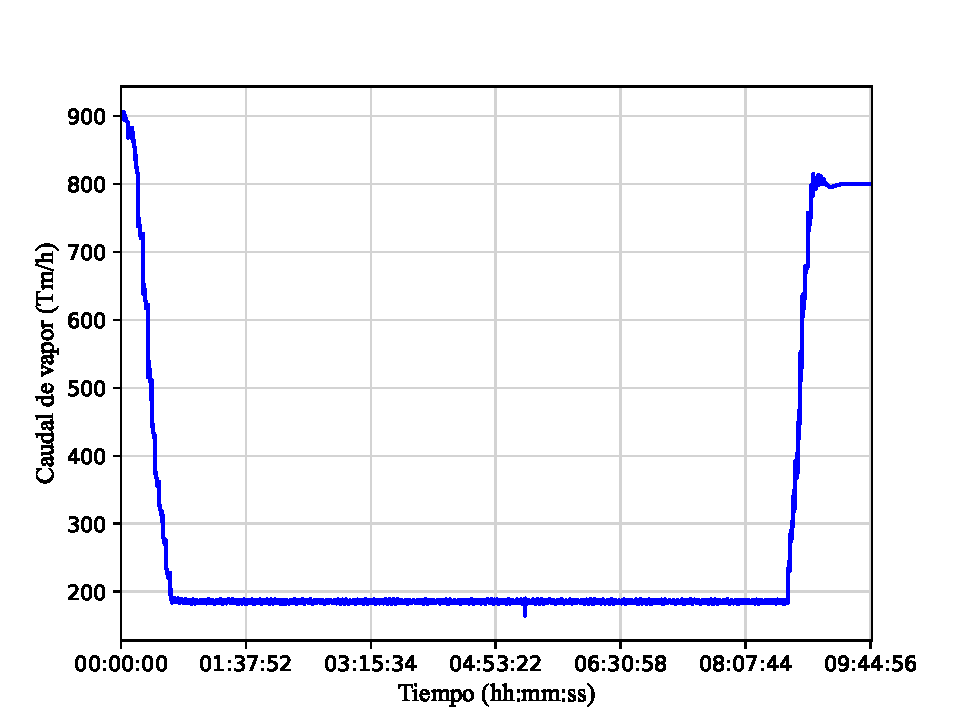
\includegraphics[width=0.5\linewidth]{content/figures/sim3_vapor.pdf}
  \caption{Posición de las válvulas de admisión de vapor (a la izquierda) y caudal de vapor que entra a la turbina (a la derecha) en la simulación de adaptación a la generación solar.}
  \label{fig:sim3_valvulas_vapor}
\end{figure}

En tercer lugar, las gráficas \ref{fig:sim3_barras_control} y \ref{fig:sim3_boro} muestran la inserción de barras de control y la curva de concentración de boro. Se van a emplear estas dos gráficas ---junto con otras tablas y curvas necesarias--- para analizar el \underline{efecto del xenón en la operación de seguimiento de carga} realizada. En concreto, se va a estudiar el comportamiento de las mismas en el periodo de baja potencia (alrededor del 22\%), en el cual la temperatura permanece en un rango de valores constante y los principales factores en juego en la aportación de reactividad positiva o negativa son los bancos de control, la concentración de ácido bórico y la concentración de xenón.

\begin{figure}[!h]
  \centering
  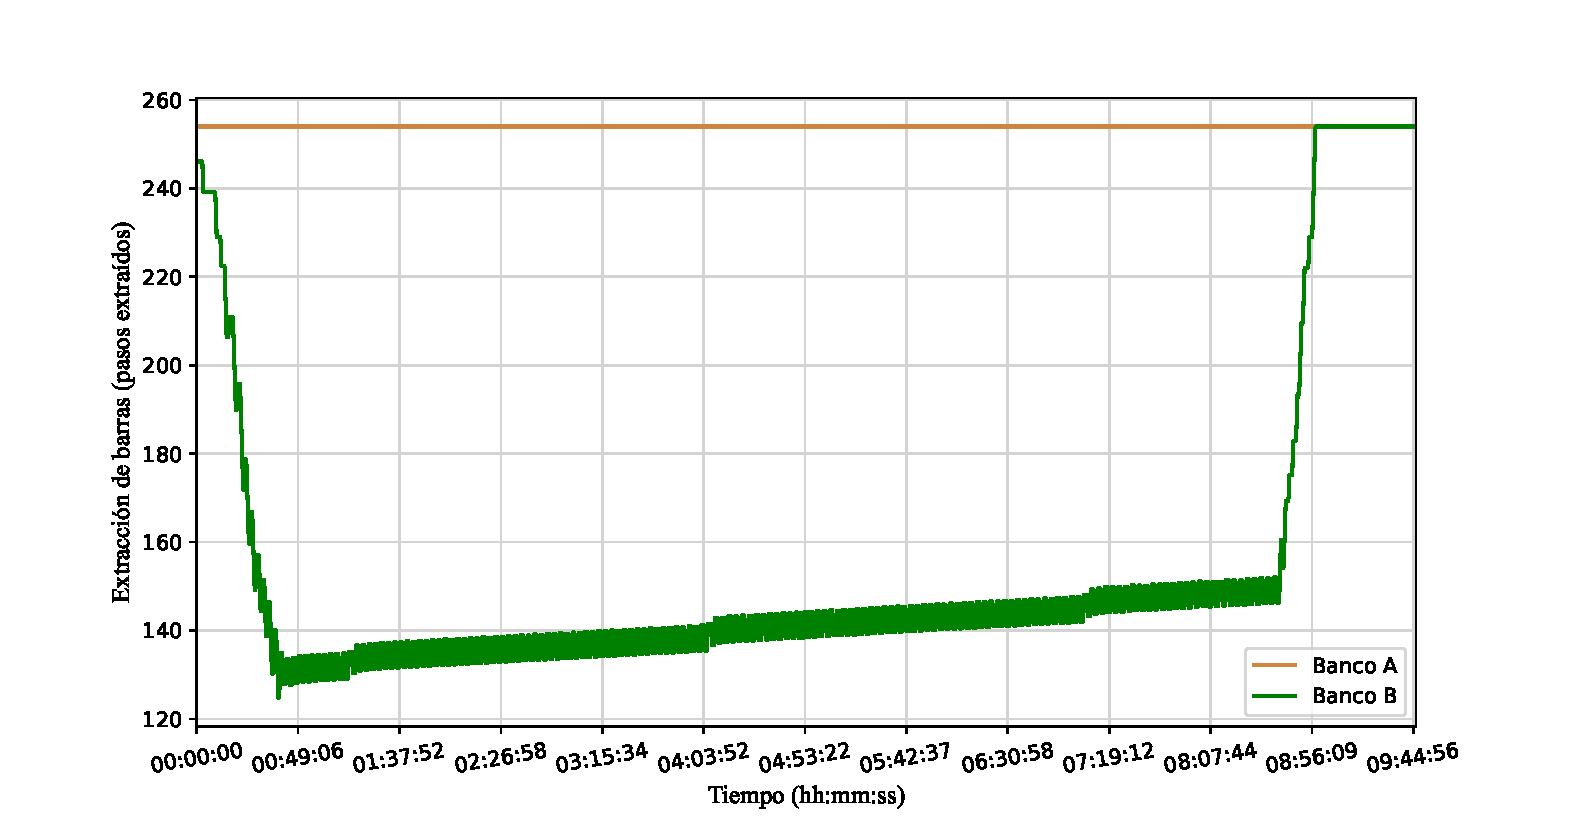
\includegraphics[width=0.95\textwidth]{content/figures/sim3_barras_control.pdf}
  \caption{Inserción de las barras de control, junto con los puntos inicial y final del análisis de reactividad realizado en la simulación de adaptación a la generación solar.}
  \label{fig:sim3_barras_control}
\end{figure}

\begin{figure}[!h]
  \centering
  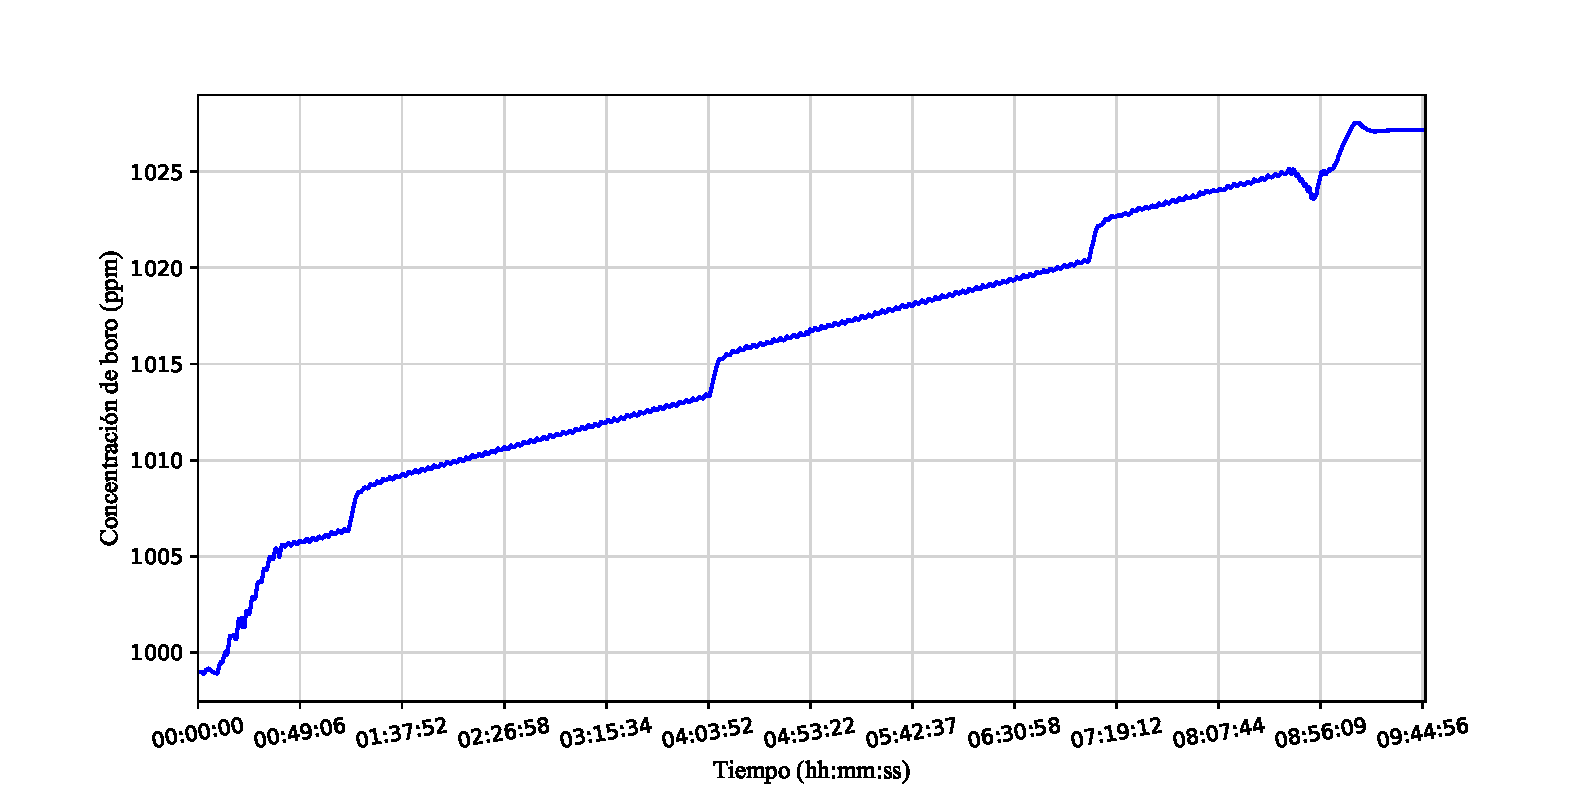
\includegraphics[width=0.95\textwidth]{content/figures/sim3_boro.pdf}
  \caption{Variación en la concentración de boro en el circuito primario en la simulación de adaptación a la generación solar.}
  \label{fig:sim3_boro}
\end{figure}

\begin{itemize}
  \item Por una parte, se observa en la figura \ref{fig:sim3_barras_control} que el banco B de las barras de control inicialmente se inserta 116 pasos hasta que la potencia nuclear alcanza aproximadamente el 22\%. En ese instante, las barras se encuentran a 130 pasos extraídos, pero estas se van extrayendo progresivamente ---aunque la potencia siga alrededor del 22\%--- hasta alcanzar un nivel de extracción de 146 pasos justo antes de comenzar la subida de potencia. Resulta así una extracción de 16 pasos a potencia constante. Interpolando los valores integrales de reactividad negativa introducida por las barras de control (tabla \ref{tab:tabla_reactividad_barras_control}), se obtiene que los 130 pasos extraídos en el punto inicial a bajas potencias corresponden a -818,228 pcm, y los 146 pasos extraídos del punto final corresponden a -662,43 pcm. Así, resulta una \textbf{introducción de reactividad positiva de 155,8 pcm por las barras de control}.
  
  \begin{table}[]
    \centering
    \vspace{-0.4cm}
    \resizebox{0.6\textwidth}{!}{%
    \begin{tabular}{|cc|c|}
    \hline
    \rowcolor[HTML]{ECF4FF} 
    \multicolumn{2}{|c|}{\cellcolor[HTML]{ECF4FF}\textbf{PASOS EXTRAÍDOS}} & \textbf{VALOR INTEGRAL}              \\ \hline
    \rowcolor[HTML]{FFCCC9} 
    \multicolumn{1}{|c|}{\cellcolor[HTML]{FFCCC9}\textbf{A}}  & \textbf{B} & \cellcolor[HTML]{FFCE93}\textbf{pcm} \\ \hline
    \multicolumn{1}{|c|}{254} & 124 & 880,1 \\ \hline
    \multicolumn{1}{|c|}{254} & 134 & 777   \\ \hline
    \multicolumn{1}{|c|}{254} & 144 & 680,5 \\ \hline
    \multicolumn{1}{|c|}{254} & 154 & 590   \\ \hline
    \end{tabular}
    }
    \caption{Tabla recortada de los valores integrales de reactividad negativa introducida en función de los pasos extraídos de los bancos A y B con solape de la Central Nuclear de Zorita, \acrshort{bol}, HFP y EqXe (\cite{enusa_1998}).}
    \label{tab:tabla_reactividad_barras_control}
    \end{table}
  
  \vspace{-0.4cm}
  \item Por otra parte, tal y como se ha explicado en el apartado \ref{metodos_seguimiento_de_carga}, la gran ventaja del empleo del ácido bórico es que, a pesar de ser muy lento, compensa los desequilibrios en la distribución del flujo neutrónico a lo largo del núcleo derivados de la introducción de las barras de control. Por eso, la figura \ref{fig:sim3_boro} muestra una tendencia lenta pero creciente de la concentración de boro. Ya que el sistema intenta que el ácido bórico inyecte la mayor cantidad posible de reactividad negativa. Teniendo en cuenta que el boro aporta una reactividad negativa alrededor de -10 pcm/ppm, como la concentración de boro aumenta en 20 ppm entre el punto inicial y final de la ``estabilización'' al 22\% de potencia, \textbf{se introduce una reactividad negativa de -200 pcm debida al boro}.
  
  \item Por último, para obtener una aproximación cuantitativa de la reactividad negativa introducida por el aumento en la concentración de xenón debido al gran descenso de potencia efectuado, se obtiene la inserción de reactividad negativa al inicio y al final de la ``estabilización'' al 20\% de potencia a partir de la figura \ref{fig:reactividad_xenon_disparo}. Se hace la aproximación de que la disminución realizada desde el 100\% hasta el 22\% de potencia es análoga al disparo a partir del 75\% de potencia, utilizando la curva de este último porcentaje en la figura \ref{fig:reactividad_xenon_disparo} para la obtención de la información deseada. En el punto inicial de la ``estabilización'' el xenón introduce una reactividad negativa de -2700 pcm y en el punto final ---pasadas 8,1 horas después de la caída de potencia--- introduce una reactividad negativa de -4450 pcm. Por tanto, entre el punto inicial y final de la ``estabilización'', \textbf{el xenón introduce una reactividad negativa de -1750 pcm}.
  
  \begin{figure}[!h]
    \centering
    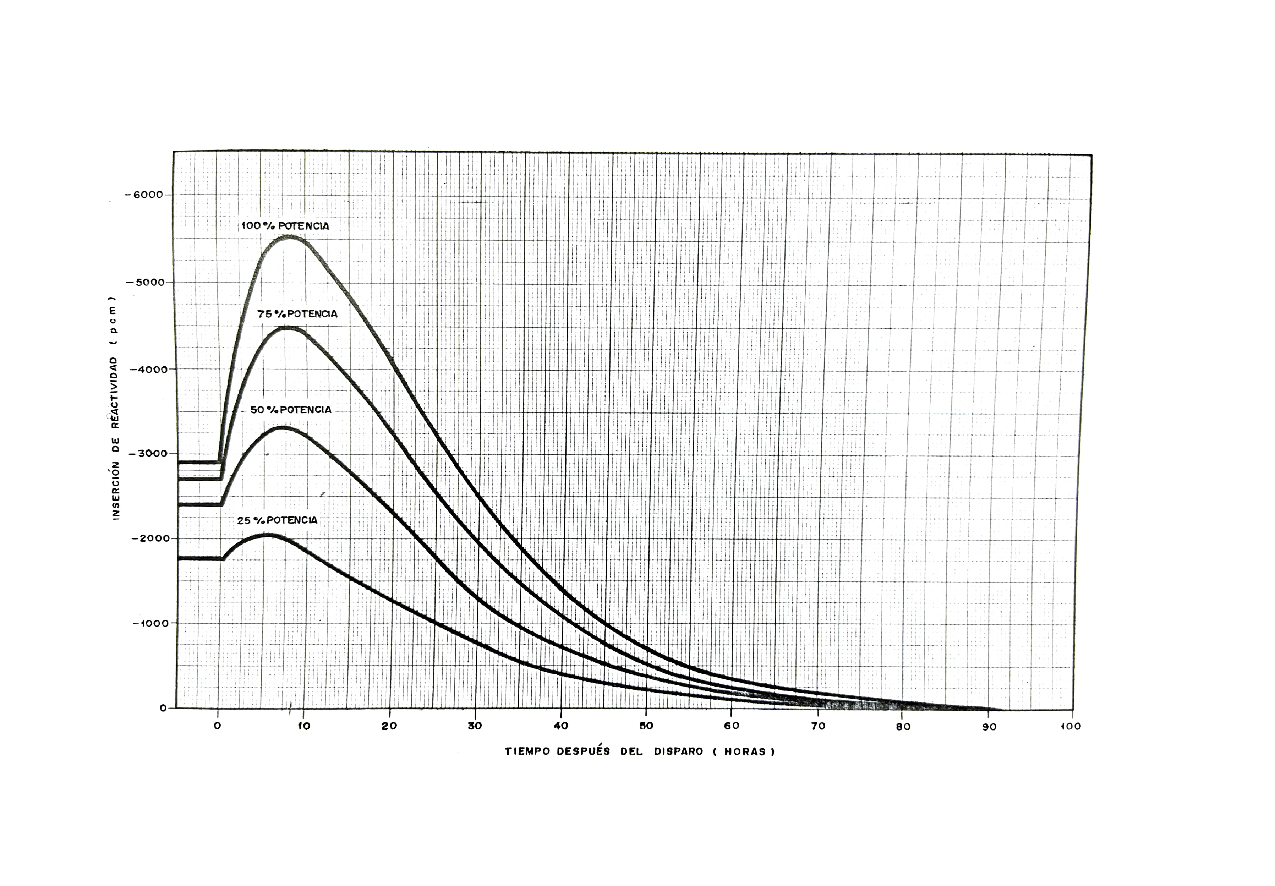
\includegraphics[width=0.8\textwidth]{content/figures/reactividad_xenon_disparo.pdf}
    \caption{Inserción de reactividad debida al xenón, después de un disparo al \acrshort{bol} a distintos niveles de potencia (\cite{documentacion_sgiz}).}
    \label{fig:reactividad_xenon_disparo}
  \end{figure}

  \item Llegados a este punto, se resumen a continuación los resultados cuya obtención se ha detallado en los puntos anteriores:
  
  \begin{table}[h]
    \centering
    \resizebox{0.65\textwidth}{!}{%
    \begin{tabular}{c|c|c|c|}
    \cline{2-4}
     &
      \cellcolor[HTML]{ECF4FF}\textbf{\begin{tabular}[c]{@{}c@{}}Punto inicial\\ (0:36:34)\end{tabular}} &
      \cellcolor[HTML]{ECF4FF}\textbf{\begin{tabular}[c]{@{}c@{}}Punto final\\ (8:39:58)\end{tabular}} &
      \cellcolor[HTML]{ECF4FF}\textbf{Variación} \\ \hline
    \multicolumn{1}{|c|}{\cellcolor[HTML]{FFCCC9}\begin{tabular}[c]{@{}c@{}}Extracción banco de\\ barras de control B\\ (pasos extraídos)\end{tabular}} &
      130 &
      146 &
      16 \\ \hline
    \multicolumn{1}{|c|}{\cellcolor[HTML]{FFCCC9}\begin{tabular}[c]{@{}c@{}}Concentración de\\ boro (ppm)\end{tabular}} &
      1005,15 &
      1024,93 &
      19,78 \\ \hline
    \multicolumn{1}{|c|}{\cellcolor[HTML]{ACEBAB}\begin{tabular}[c]{@{}c@{}}Reactividad introducida\\ por las barras de control\\ (pcm)\end{tabular}} &
      -818,228 &
      -662,43 &
      \textbf{155,8} \\ \hline
    \multicolumn{1}{|c|}{\cellcolor[HTML]{ACEBAB}\begin{tabular}[c]{@{}c@{}}Reactividad introducida\\ por el ácido bórico\\ (pcm)\end{tabular}} &
      -10051,5 &
      -10249,3 &
      \textbf{-197,8} \\ \hline
    \multicolumn{1}{|c|}{\cellcolor[HTML]{ACEBAB}\begin{tabular}[c]{@{}c@{}}Reactividad introducida\\ por el xenón (pcm)\end{tabular}} &
      -2700 &
      -4450 &
      \textbf{-1750} \\ \hline
    \multicolumn{1}{|c|}{\cellcolor[HTML]{ACEBAB}\begin{tabular}[c]{@{}c@{}}Reactividad total\\ aportada (pcm)\end{tabular}} &
      -13569,73 &
      -15361,73 &
      \cellcolor[HTML]{FFFFC7}\textbf{-1792} \\ \hline
    \end{tabular}
    }
    \caption{Resumen de los cálculos de reactividad realizados para la obtención de la variación en la reactividad total entre el punto inicial y final de la``estabilización'' al 20\% de potencia.}
    \label{tab:calculos_reactividad}
    \end{table}
  
    \item De los resultados obtenidos, se observa que la reactividad negativa introducida por barras de control, boro y xenón en el punto inicial analizado es inferior a la reactividad negativa global en el punto final. Este comportamiento no es para nada el esperado, ya que ---a temperatura constante y \acrshort{bol}--- lo propio sería que la reactividad negativa total introducida por estos medios fuera la misma en el punto inicial y final, con una variación prácticamente nula. El hecho más probable de ser el causante de este resultado inesperado es la leve extracción de barras de control que se ha realizado entre ambos puntos del análisis (tan solo 16 pasos). Tras investigar el asunto, parece que los desarrolladores del simulador optaron por emplear un modelo con cinética puntual que no permite el cálculo de los efectos del xenón ---y, por tanto, no los tiene en cuenta--- en transitorios largos. Esto se debe a la mayor simplicidad y velocidad de cálculo para aquella época frente al modelado 3D.
\end{itemize}



Por último, en las figuras \ref{fig:sim3_gen_vapor_camara_imp} y \ref{fig:sim3_presionador} se muestra la evolución de las variables de mayor interés del generador de vapor y del presionador. De ellas, puede extraerse la siguiente información:

\begin{itemize}
  \item Tal y como se ha mencionado ya en la simulación corta, el comportamiento de la presión de la cámara de impulsos es solidario con el de la potencia nuclear, mientras que el de la presión del generador de vapor es opuesto al de la potencia nuclear. Por una parte, al cerrar parcialmente las válvulas de control para disminuir la potencia, a parte de disminuir el gasto de vapor entrante a la turbina, el vapor sufre un proceso de laminación, por lo que disminuye su presión en la cámara de impulsos. Por otra parte, el cierre parcial de las válvulas conlleva ---como ya se ha comentado--- una saturación del generador de vapor, lo que provoca el aumento de la presión en la admisión ---aguas arriba de las válvulas---y, por tanto, en el propio generador de vapor.
  \item El nivel del generador de vapor sufre algunas fluctuaciones más significativas en los periodos de bajada y subida de potencia ---ya que son fases transitorias más inestables---, pero se mantiene oscilando en un rango más acotado cuando la potencia permanece prácticamente constante a un 22\%.
  \item Algo muy similar al punto anterior sucede con la presión del presionador.
  \item La disminución final en el nivel del presionador es consecuencia de la drástica disminución de temperatura explicada anteriormente (figura \ref{fig:sim3_temperaturas}), ante la cual no se ha encontrado otra explicación más que un posible error en la simulación. 
  
  Al disminuir la $T_{med}$ del primario, disminuye consecuentemente la presión en el presionador. Asimismo, el agua se contrae y disminuye el nivel del presionador. En este caso, es por tanto necesario disminuir el caudal de descarga del sistema de control químico y volumétrico, para mantener los niveles de agua borada en el primario. Cuando la $T_{med}$ aumenta, sucede totalmente lo contrario.
\end{itemize}

\begin{figure}[!h]
  \centering
  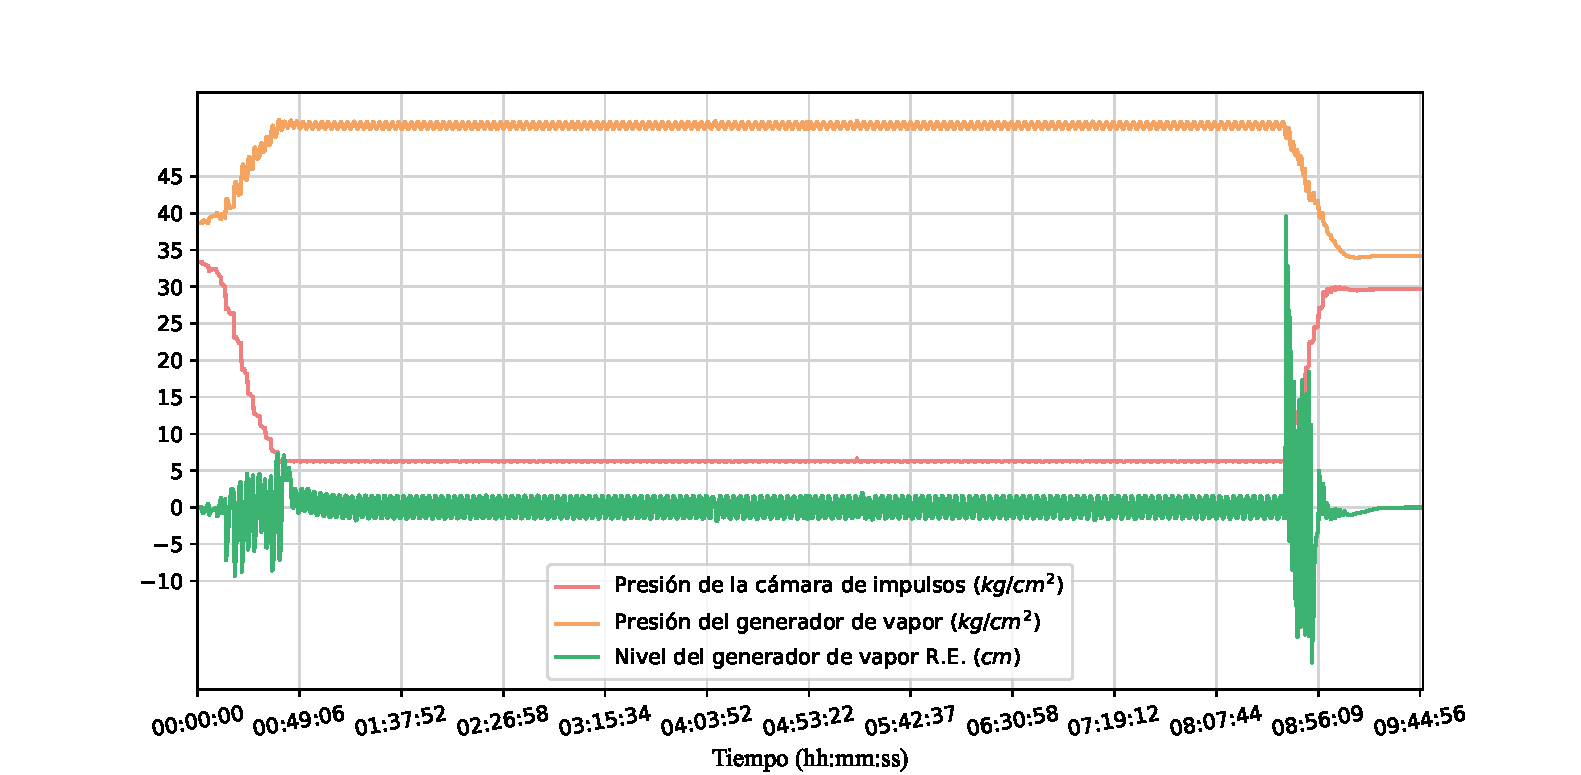
\includegraphics[width=\textwidth]{content/figures/sim3_gen_vapor_camara_imp.pdf}
  \caption{Propiedades del generador de vapor y de la cámara de impulsos.}
  \label{fig:sim3_gen_vapor_camara_imp}
\end{figure}

\begin{figure}[!h]
  \centering
  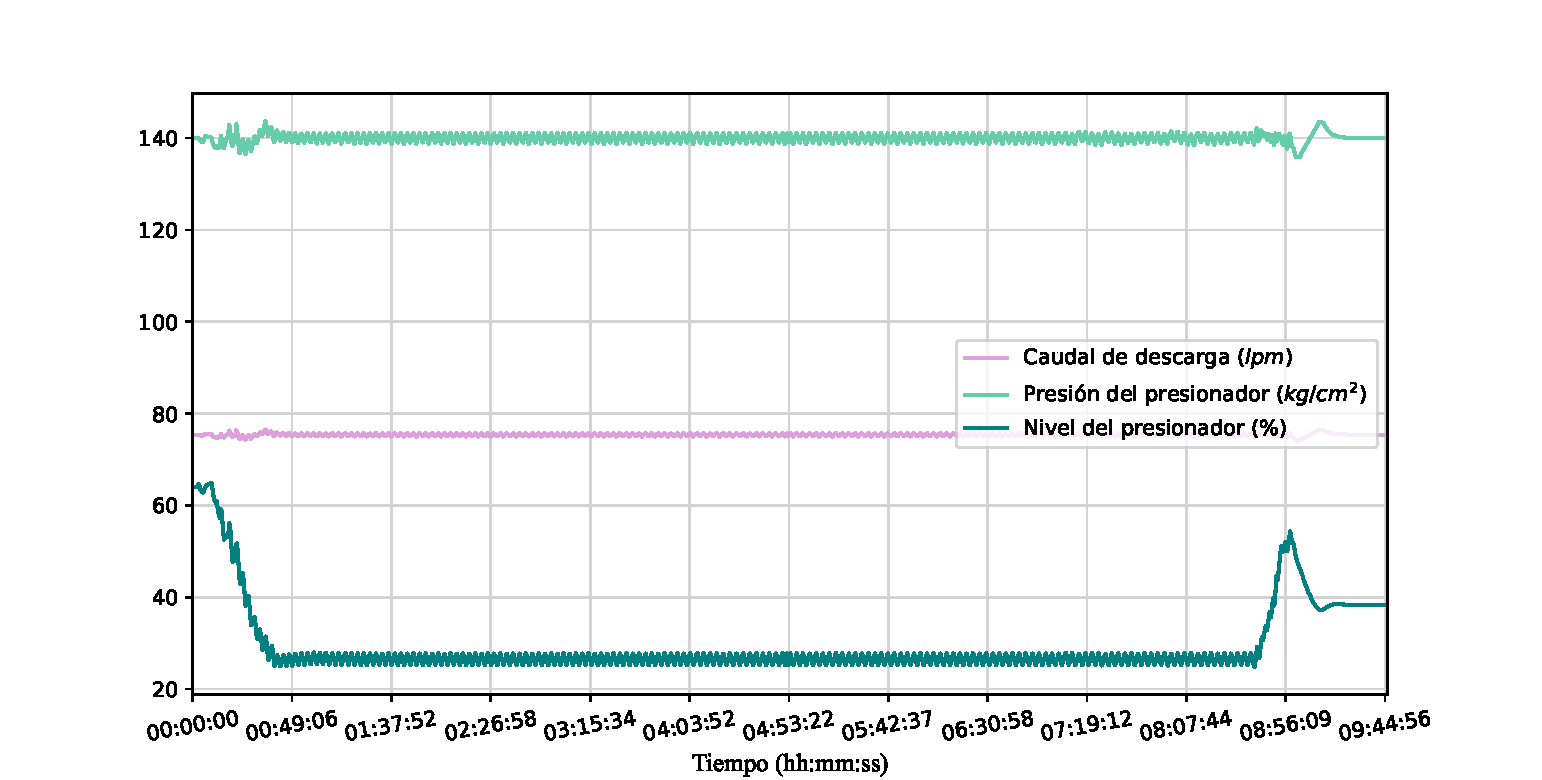
\includegraphics[width=\textwidth]{content/figures/sim3_presionador.pdf}
  \caption{Propiedades del presionador.}
  \label{fig:sim3_presionador}
\end{figure}


\newpage
\subsubsection{Adaptación a la curva de demanda eléctrica}

\textit{Simulación de 15 horas y 15 minutos realizada en el \acrshort{sgiz} el 17 de junio de 2024.}

\paragraph{Contextualización}

Red Eléctrica Española realiza un seguimiento instantáneo de la demanda eléctrica total, registrando la demanda de todos los días del año. Tomando un día cualquiera ---el 24 de abril de 2024---, se procede a realizar un seguimiento de carga de la curva de demanda eléctrica nacional entre las 14:00 del día 24 y las 5:15 del día 25:

\begin{figure}[!h]
  \centering
  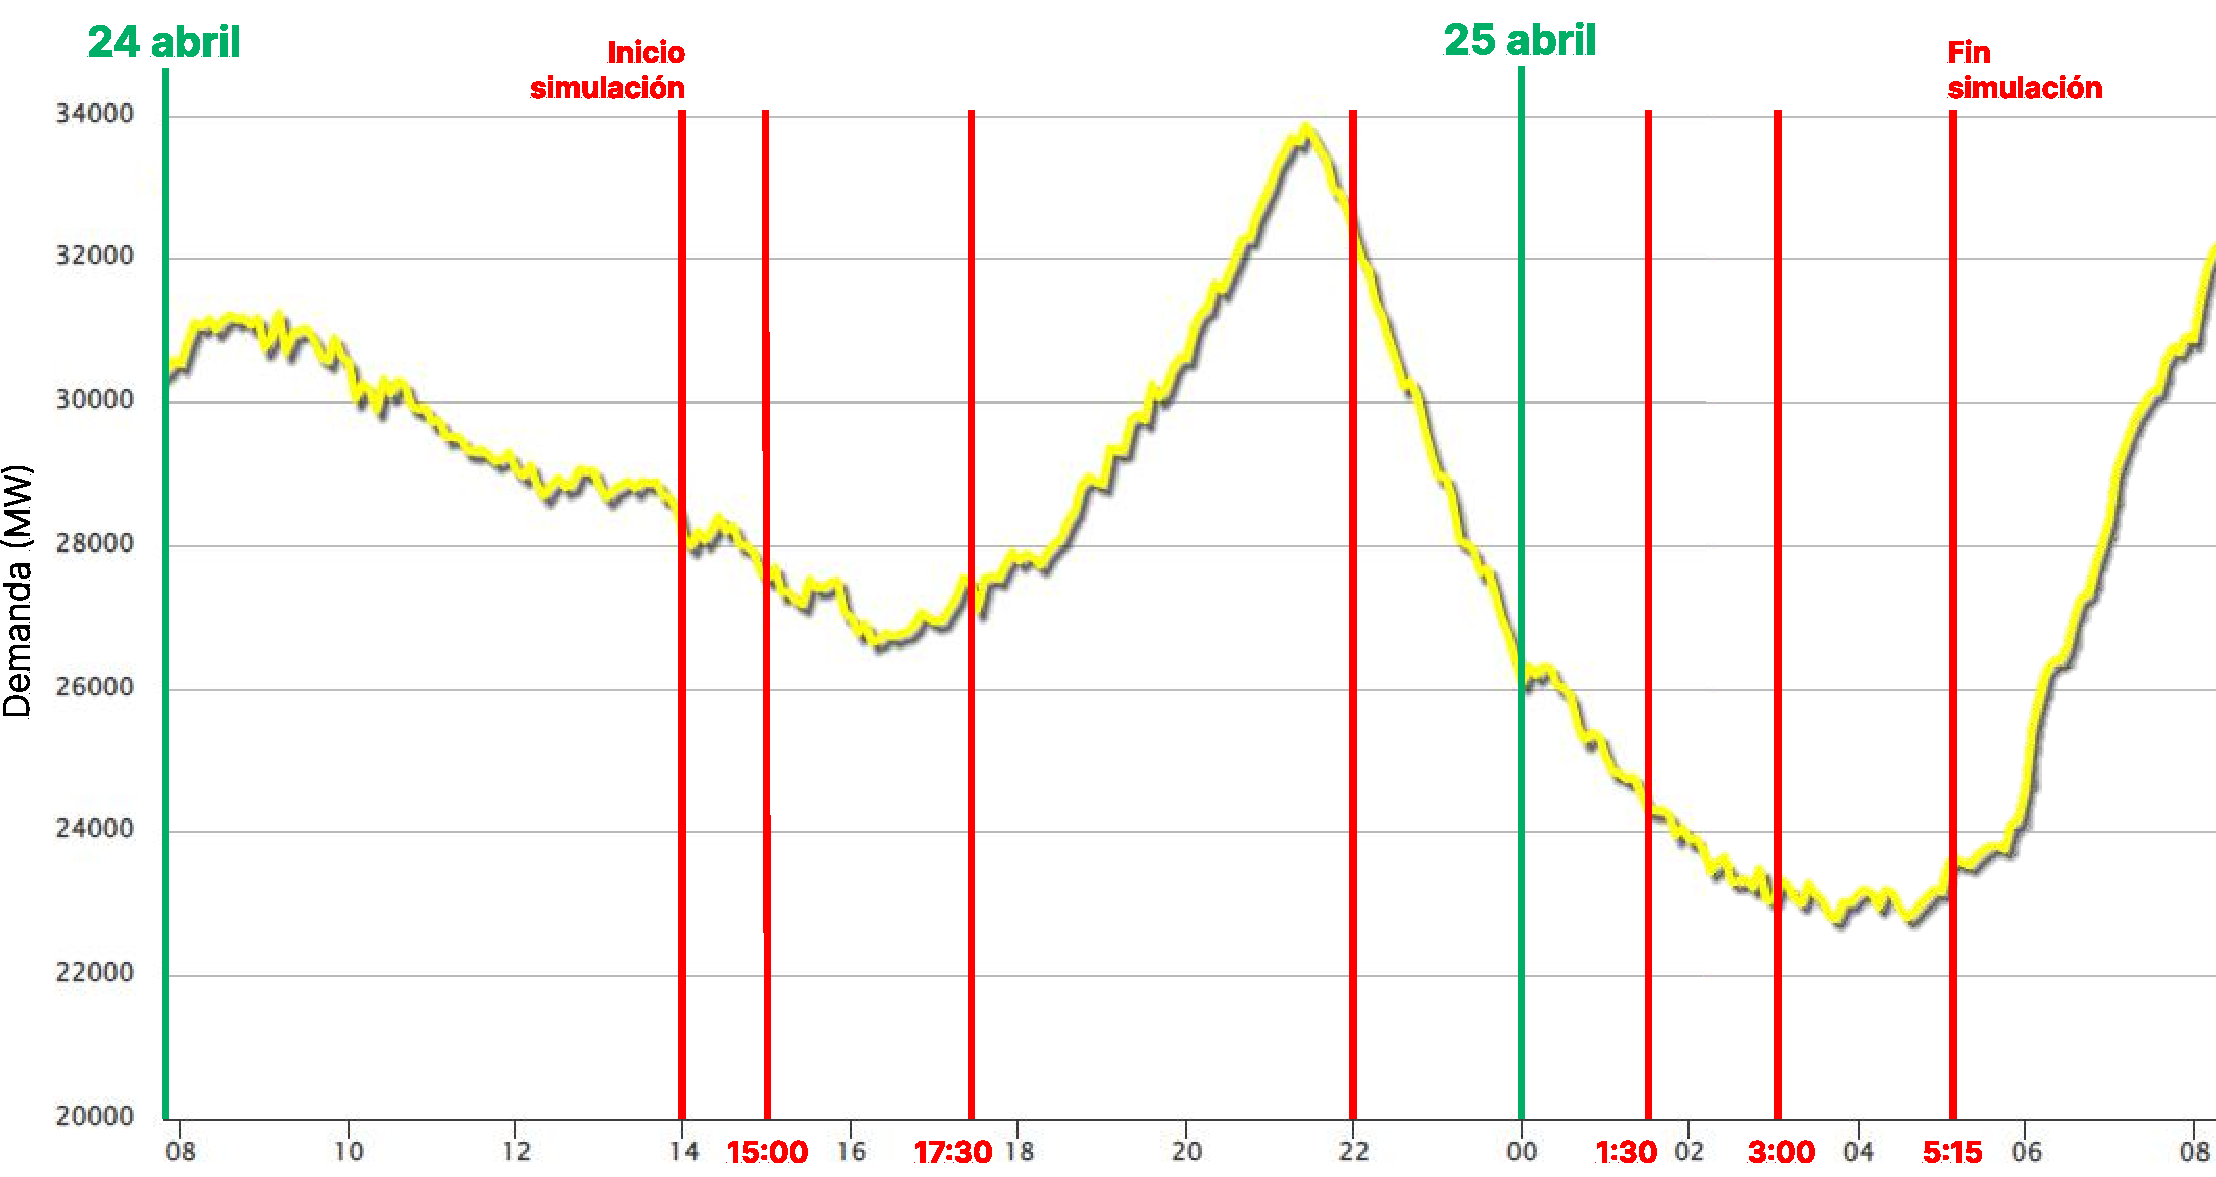
\includegraphics[width=0.9\textwidth]{content/figures/curva_demanda.pdf}
  \caption{Curva de demanda eléctrica en España de los días 24 y 25 de abril de 2024. Se detallan en rojo los momentos importantes de la simulación (\cite{ree_demanda}).}
  \label{fig:curva_demanda}
\end{figure}

\begin{figure}[!h]
  \centering
  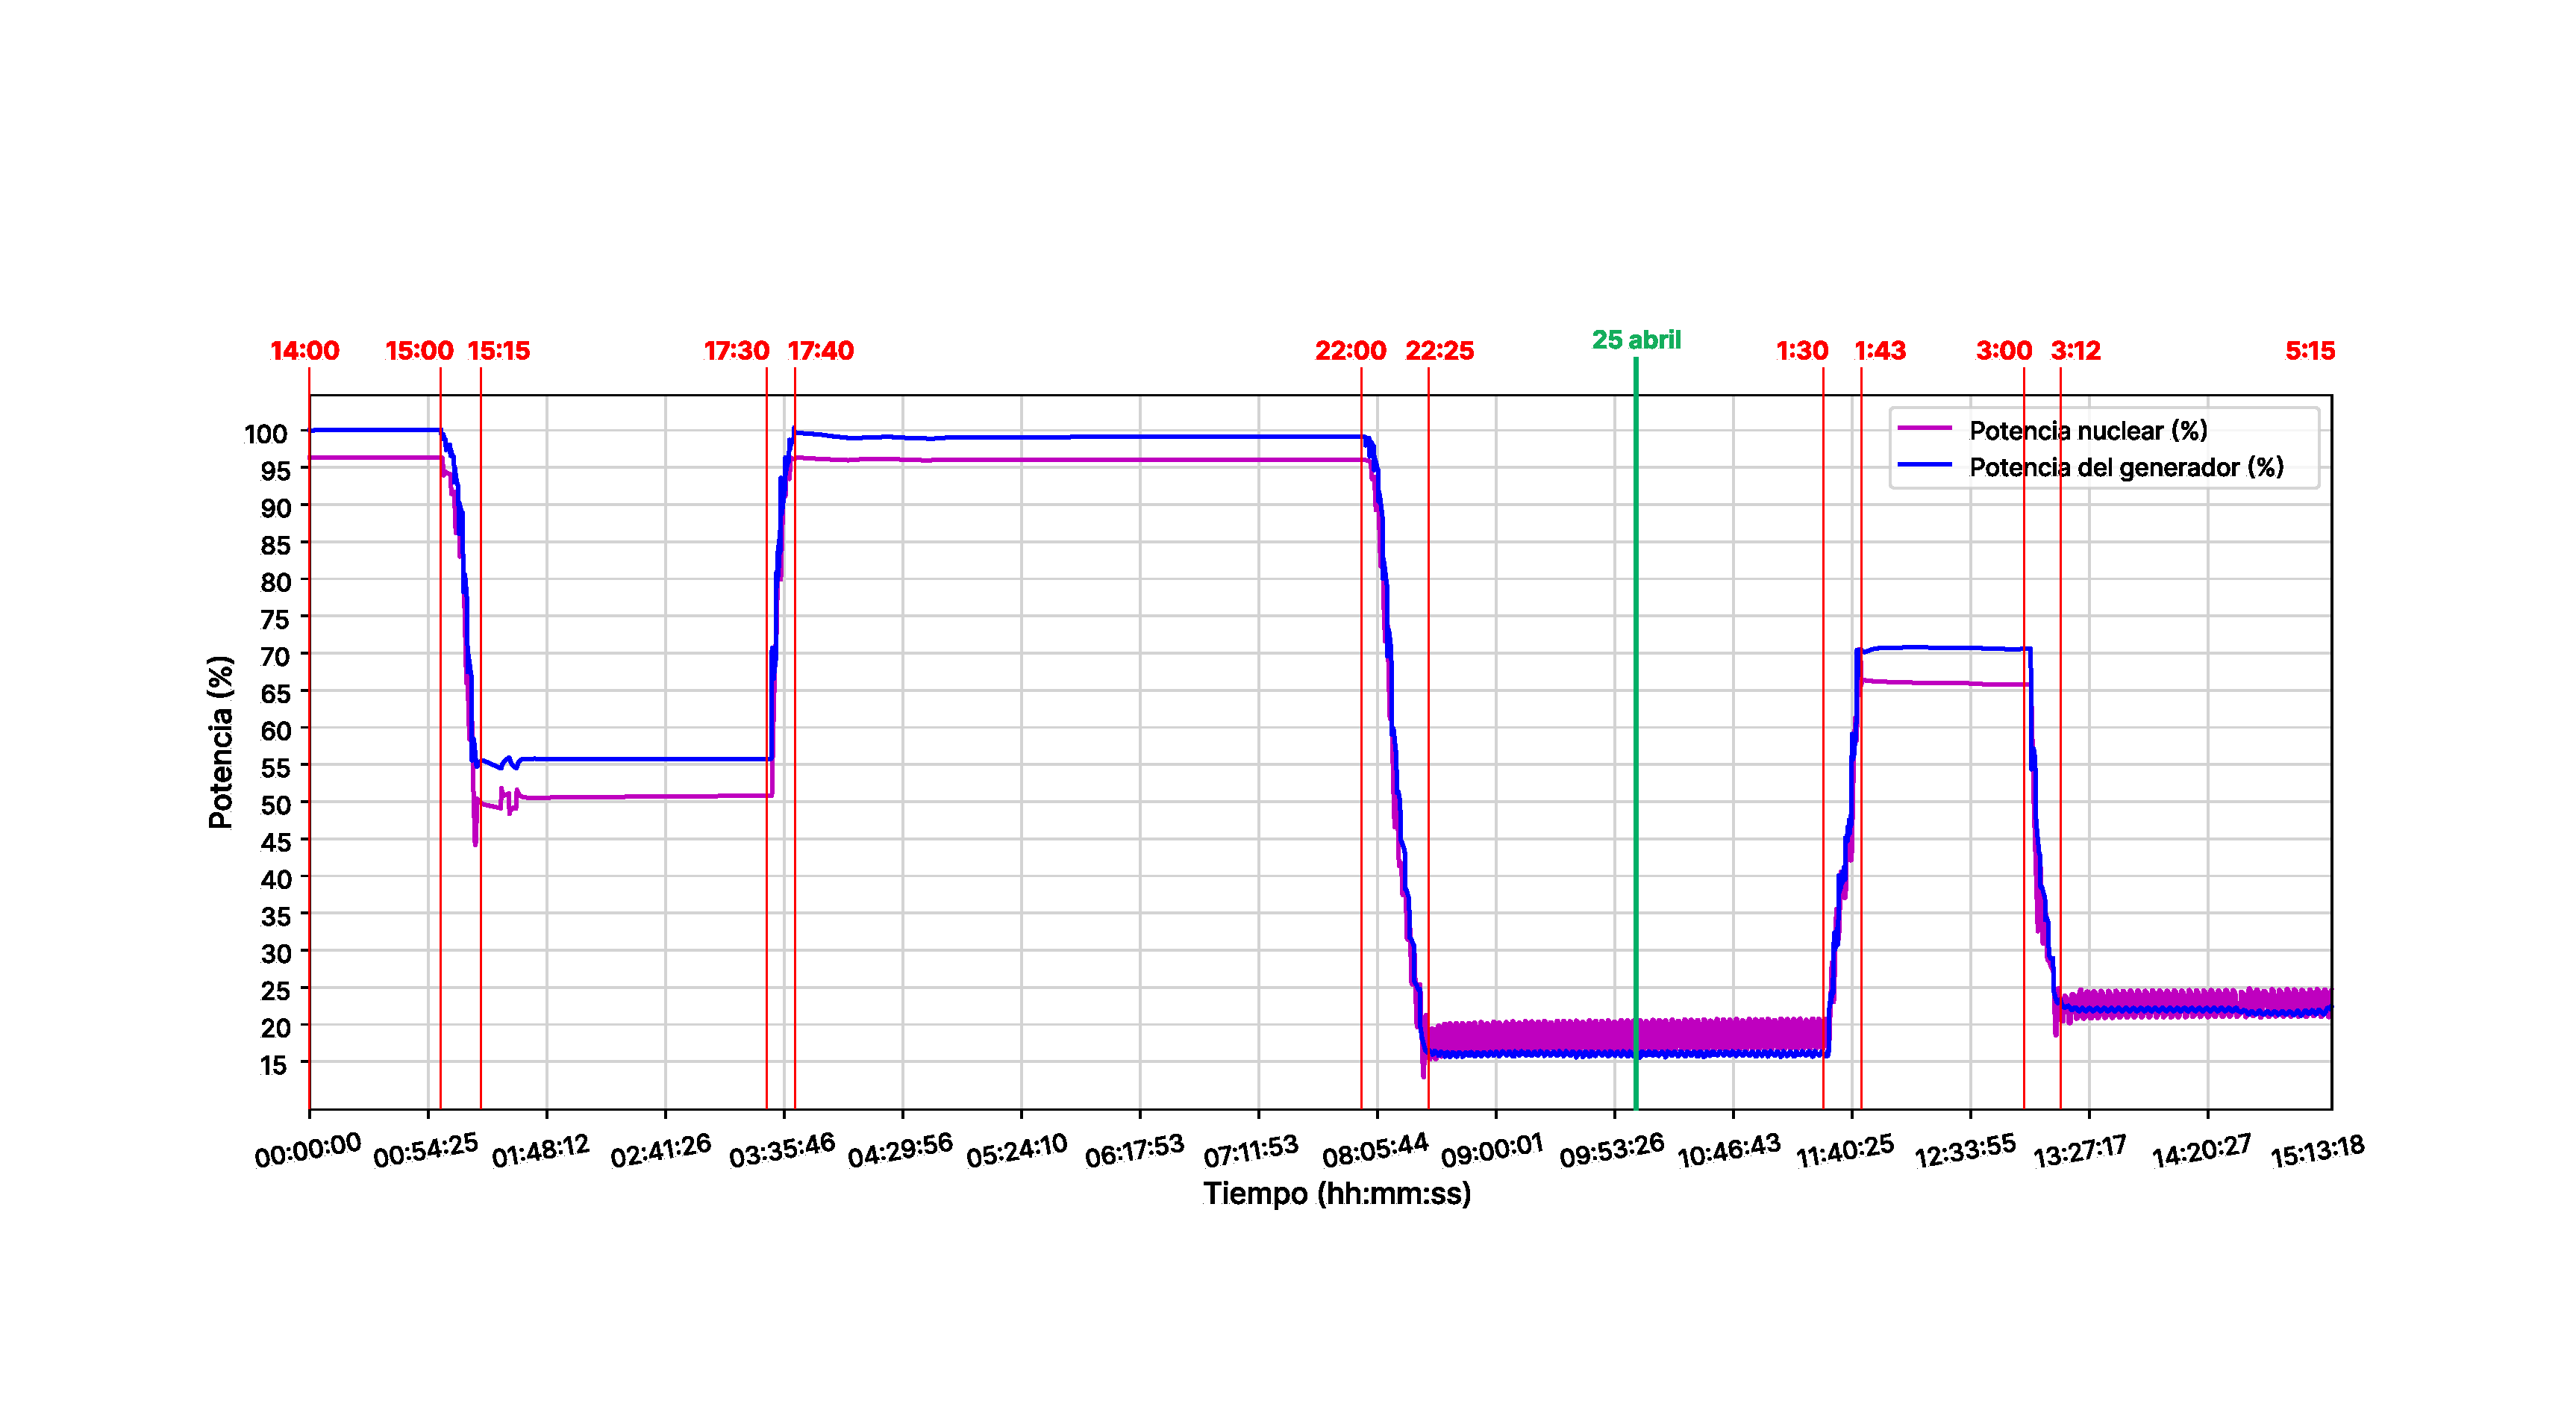
\includegraphics[width=\textwidth]{content/figures/sim4_potencias_contextualizacion.pdf}
  \caption{Variaciones de potencia para el seguimiento de la curva de demanda entre los días 24 y 25 de abril de 2024. Se detallan en rojo los momentos importantes de la simulación.}
  \label{fig:sim4_potencias_contextualizacion}
\end{figure}

A continuación, se detallan cronológicamente los cambios en la demanda eléctrica y en la producción renovable, que conllevan un consecuente seguimiento de carga:

\begin{itemize}
  \item \underline{14.00 - 15.00 del 24 de abril:} La demanda de energía eléctrica es elevada pero va disminuyendo progresivamente. Se mantiene la central a potencia nominal.
  \item \underline{15.00 - 17.30:} Son unas horas valle en las que la demanda disminuye considerablemente. Se baja la potencia de la planta al 50\% y se mantiene esa potencia durante 2 horas y media:
  \begin{itemize}
    \item \textbf{Variación de potencia:} 46\%
    \item \textbf{Tiempo empleado:} 15 minutos
    \item \textbf{Tasa de variación de potencia:} 3,07\%/min
  \end{itemize} 
  \item \underline{17.30 - 22.00:} A partir de las 17.30 la demanda eléctrica aumenta muy considerablemente, por lo que es necesario volver a generar el 100\% de la potencia:
  \begin{itemize}
    \item \textbf{Variación de potencia:} 46\%
    \item \textbf{Tiempo empleado:} 10 minutos
    \item \textbf{Tasa de variación de potencia:} 4,6\%/min
  \end{itemize} 
  Seguidamente, se mantiene la central a potencia nominal hasta que la curva de demanda comienza a caer muy rápidamente poco antes de las 22.00 de la noche, comenzando el gran valle típico en la curva de demanda eléctrica nocturna. Por tanto, bajamos entorno al 18\% de potencia la las 22.00:
  \begin{itemize}
    \item \textbf{Variación de potencia:} 78\%
    \item \textbf{Tiempo empleado:} 55 minutos
    \item \textbf{Tasa de variación de potencia:} 3,12\%/min
  \end{itemize}
  \item \underline{22.25 - 1.30 del 25 de abril:} La potencia se mantiene entorno al 18\%.
  \item \underline{1.30 - 3.00:} Hasta el momento, toda la maniobra de seguimiento de carga se ha realizado teniendo las fuentes de energía renovable produciendo al máximo ---como es lógico, la solar ha dejado de producir por la noche---. Sin embargo, a partir de la 1.30, se produce una gran calma de viento en la península y la mayoría de aerogeneradores dejan de funcionar. Es necesario, por tanto, aumentar la potencia nuclear, aunque no hasta el 100\%, pues la demanda eléctrica sigue siendo muy baja. Se sube por tanto la potencia entorno al 66\%: 
  \begin{itemize}
    \item \textbf{Variación de potencia:} 48\%
    \item \textbf{Tiempo empleado:} 13 minutos
    \item \textbf{Tasa de variación de potencia:} 3,7\%/min
  \end{itemize}
  Tras mantenerse a ese nivel de potencia durante aproximadamente 1 hora y 15 minutos, la velocidad del viento vuelve a sus valores iniciales y la eólica vuelve a producir prácticamente al máximo. Entonces, se hace necesario disminuir la potencia de la central entorno al 22\%:
  \begin{itemize}
    \item \textbf{Variación de potencia:} 44\%
    \item \textbf{Tiempo empleado:} 12 minutos
    \item \textbf{Tasa de variación de potencia:} 3,67\%/min
  \end{itemize}
  \item \underline{1.30 - 3.00:} Por último, se mantiene el bajo nivel de potencia hasta que se finaliza la simulación a las 5.15  de la madrugada. Si esta siguiera avanzando, a partir de las 6.00 se debería volver a subir a potencia nominal.
\end{itemize}

En definitiva, se ha podido realizar con éxito y rapidez un seguimiento de la curva de demanda eléctrica nacional y de las variaciones en la producción renovable.

\paragraph{Resto de gráficas}

El objetivo fundamental de esta última simulación ha sido ---como se ha explicado anteriormente--- realizar un conjunto de maniobras completo de seguimiento de carga. Por tanto, la gráfica de mayor interés es la de la figura \ref{fig:sim4_potencias_contextualizacion}, en la cual se muestra el seguimiento de carga realizado. Aun así, se han generado el resto de gráficas de las variables más interesantes del reactor para que se pueda observar su comportamiento durante la maniobra. Una apreciación que se muestra muy claramente en estas gráficas es la que ya se ha comentado varias veces anteriormente: cuando el reactor trabaja a potencia nominal o potencias intermedias (50\% o 66\%, en este caso), el comportamiento del sistema es muy estable, mientras que a bajas potencias (18\% o 22\%, en este caso), el sistema presenta las oscilaciones propias de la inestabilidad a potencias bajas.

\begin{figure}[!h]
  \centering
  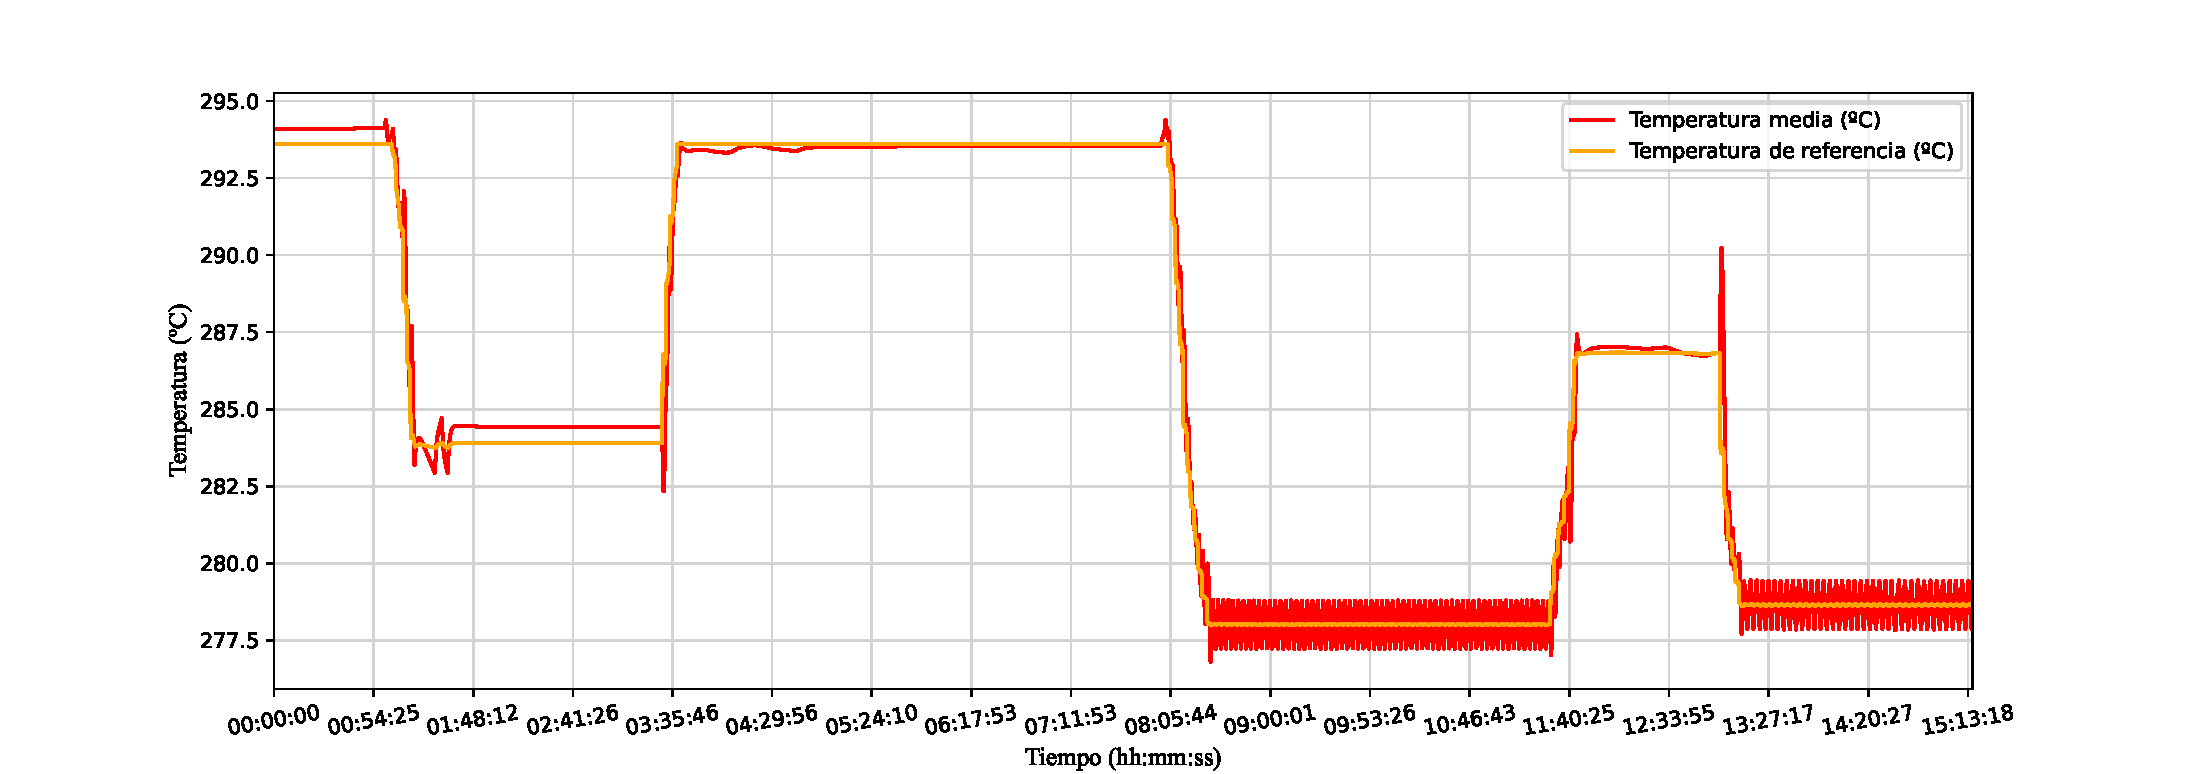
\includegraphics[width=0.9\textwidth]{content/figures/sim4_temperaturas.pdf}
  \vspace{-0.1cm}
  \caption{Variaciones de temperatura.}
  \label{fig:sim4_temperaturas}
\end{figure}

\begin{figure}[!h]
  \vspace{-0.2cm}
  \centering
  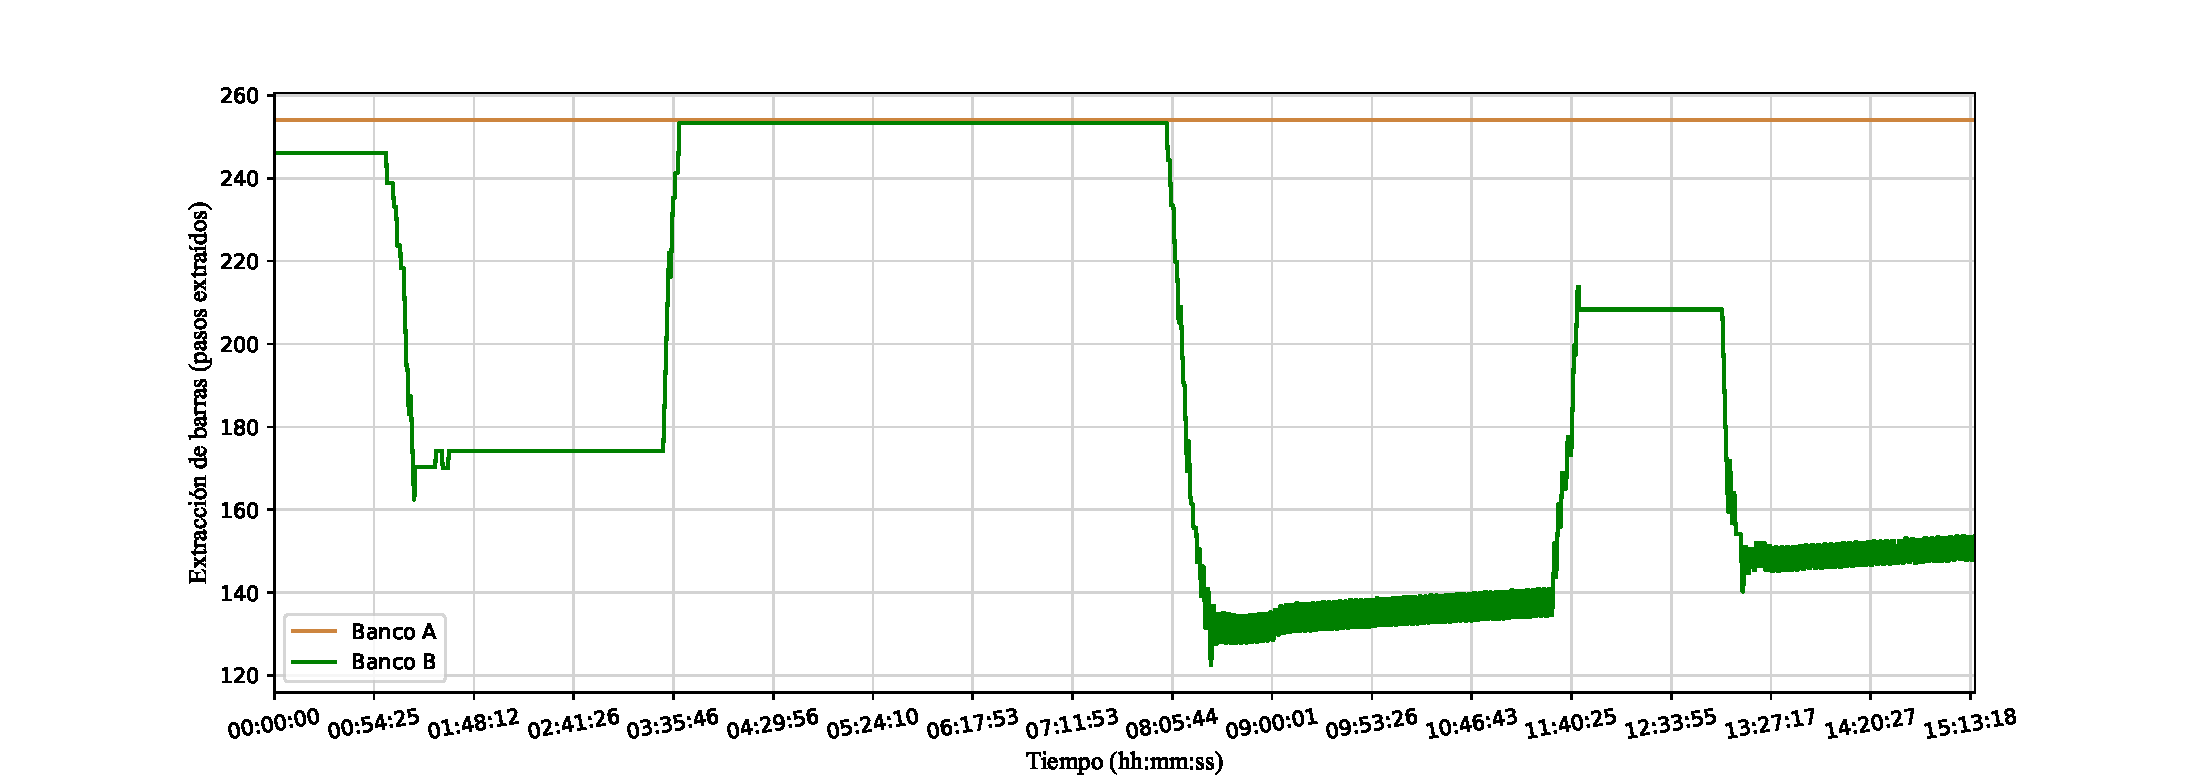
\includegraphics[width=0.9\textwidth]{content/figures/sim4_barras_control.pdf}
  \vspace{-0.1cm}
  \caption{Nivel de extracción de las barras de control.}
  \label{fig:sim4_barras_control}
\end{figure}

\begin{figure}[!h]
  \vspace{-0.2cm}
  \centering
  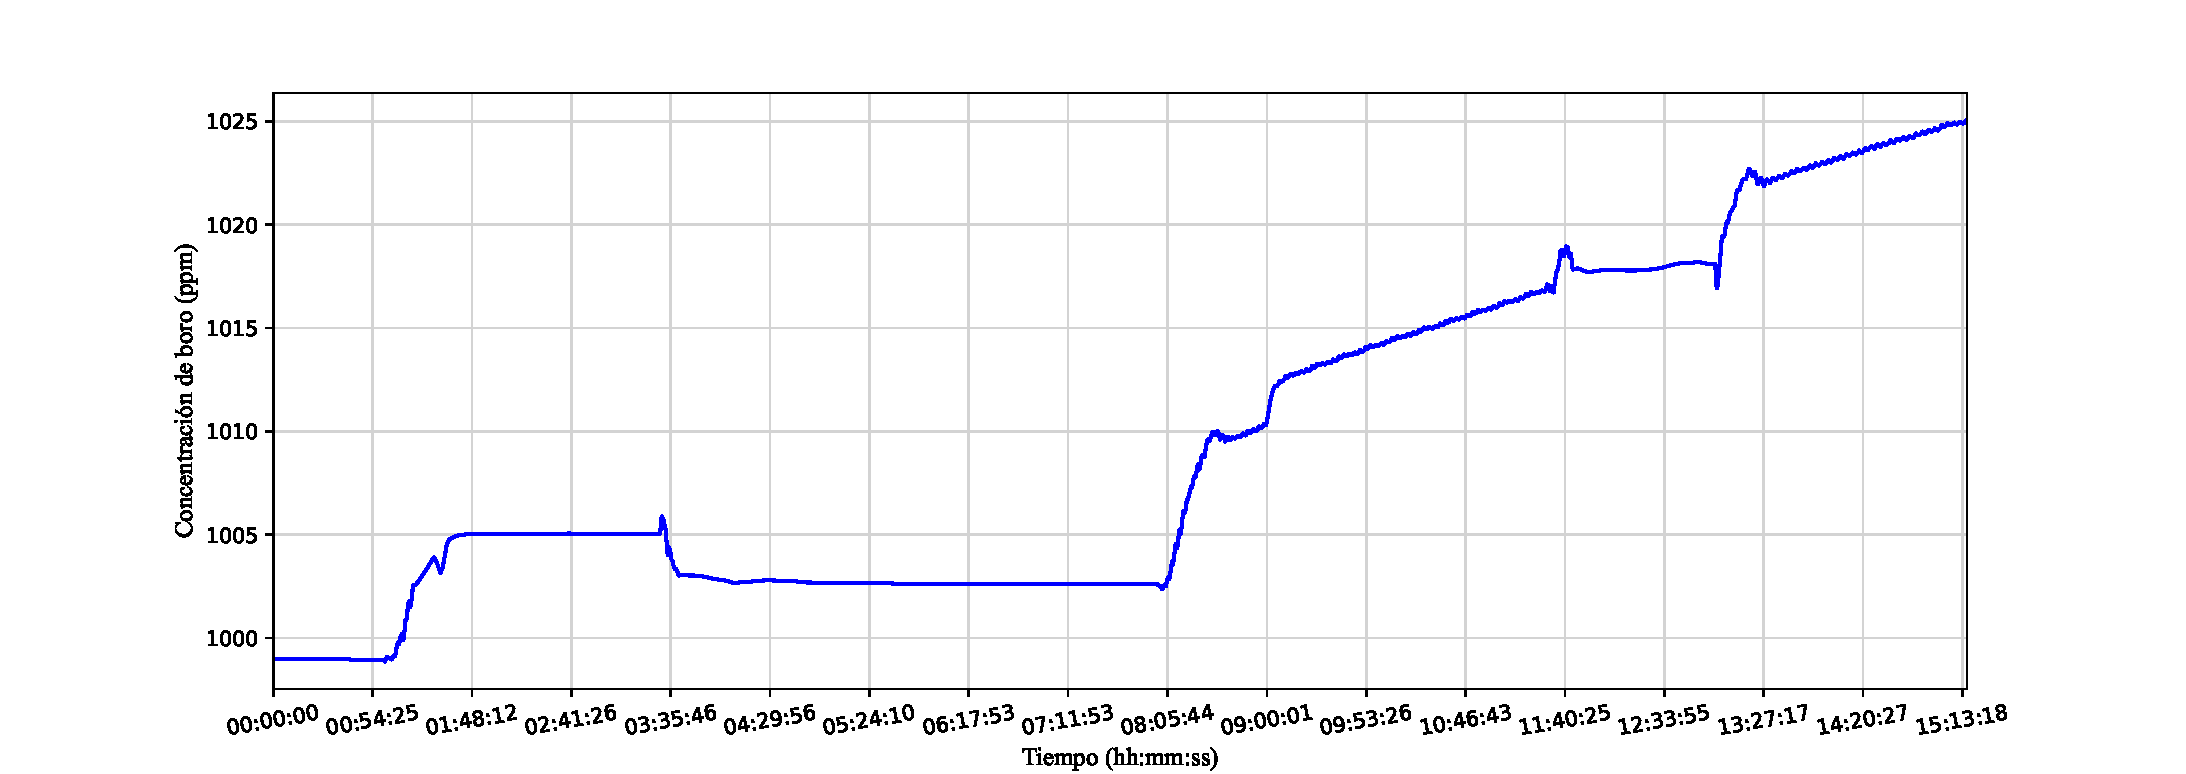
\includegraphics[width=0.9\textwidth]{content/figures/sim4_boro.pdf}
  \vspace{-0.1cm}
  \caption{Concentración de boro en el circuito primario.}
  \label{fig:sim4_boro}
\end{figure}

\begin{figure}[!h]
  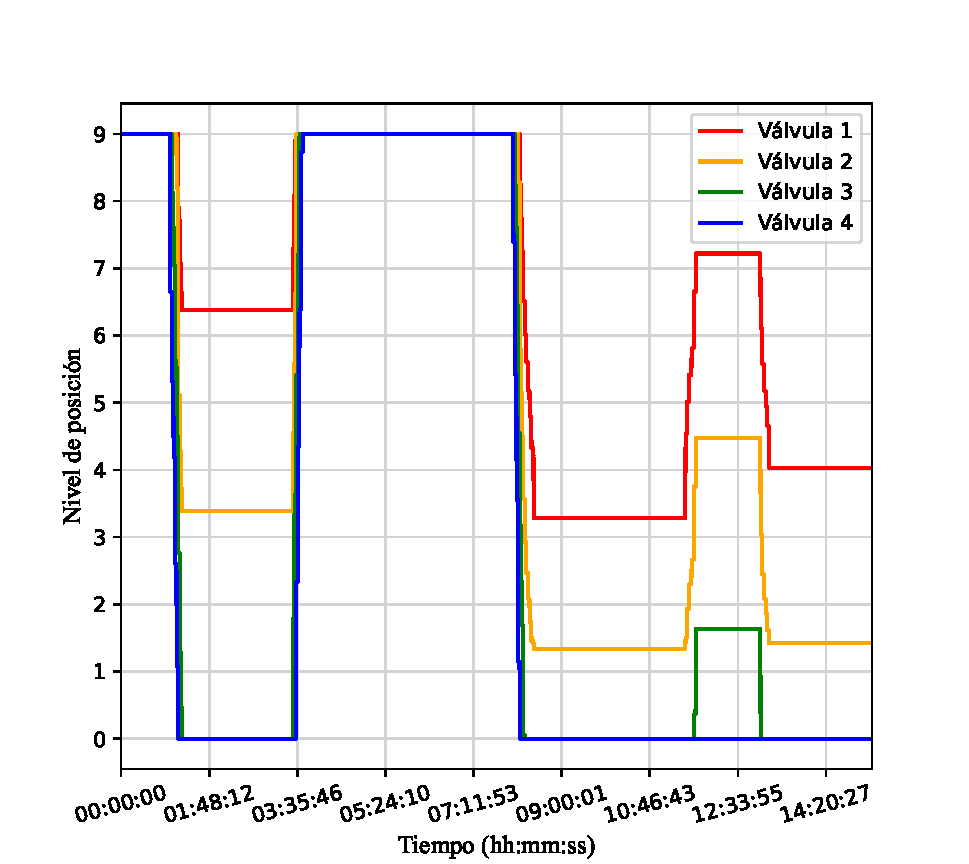
\includegraphics[width=0.5\linewidth]{content/figures/sim4_valvulas_control.pdf} 
  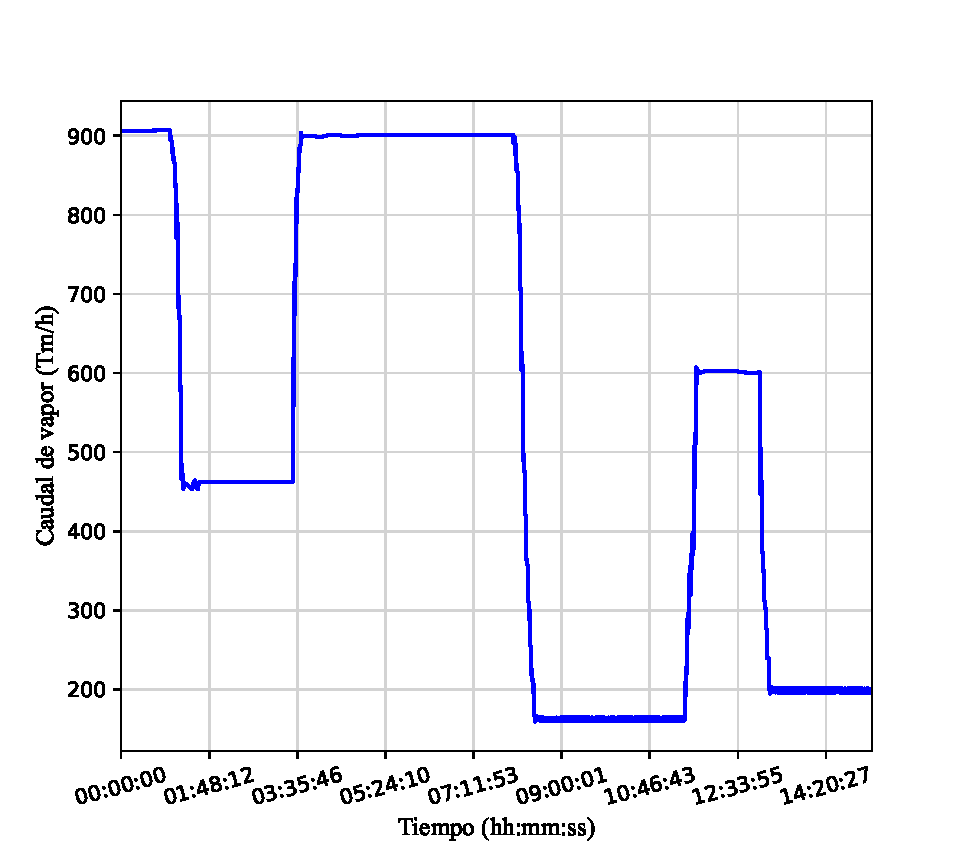
\includegraphics[width=0.5\linewidth]{content/figures/sim4_vapor.pdf}
  \caption{Posición de las válvulas de admisión de vapor (a la izquierda) y caudal de vapor que entra a la turbina (a la derecha).}
  \label{fig:sim4_valvulas_vapor}
\end{figure}

\begin{figure}[!h]
  \centering
  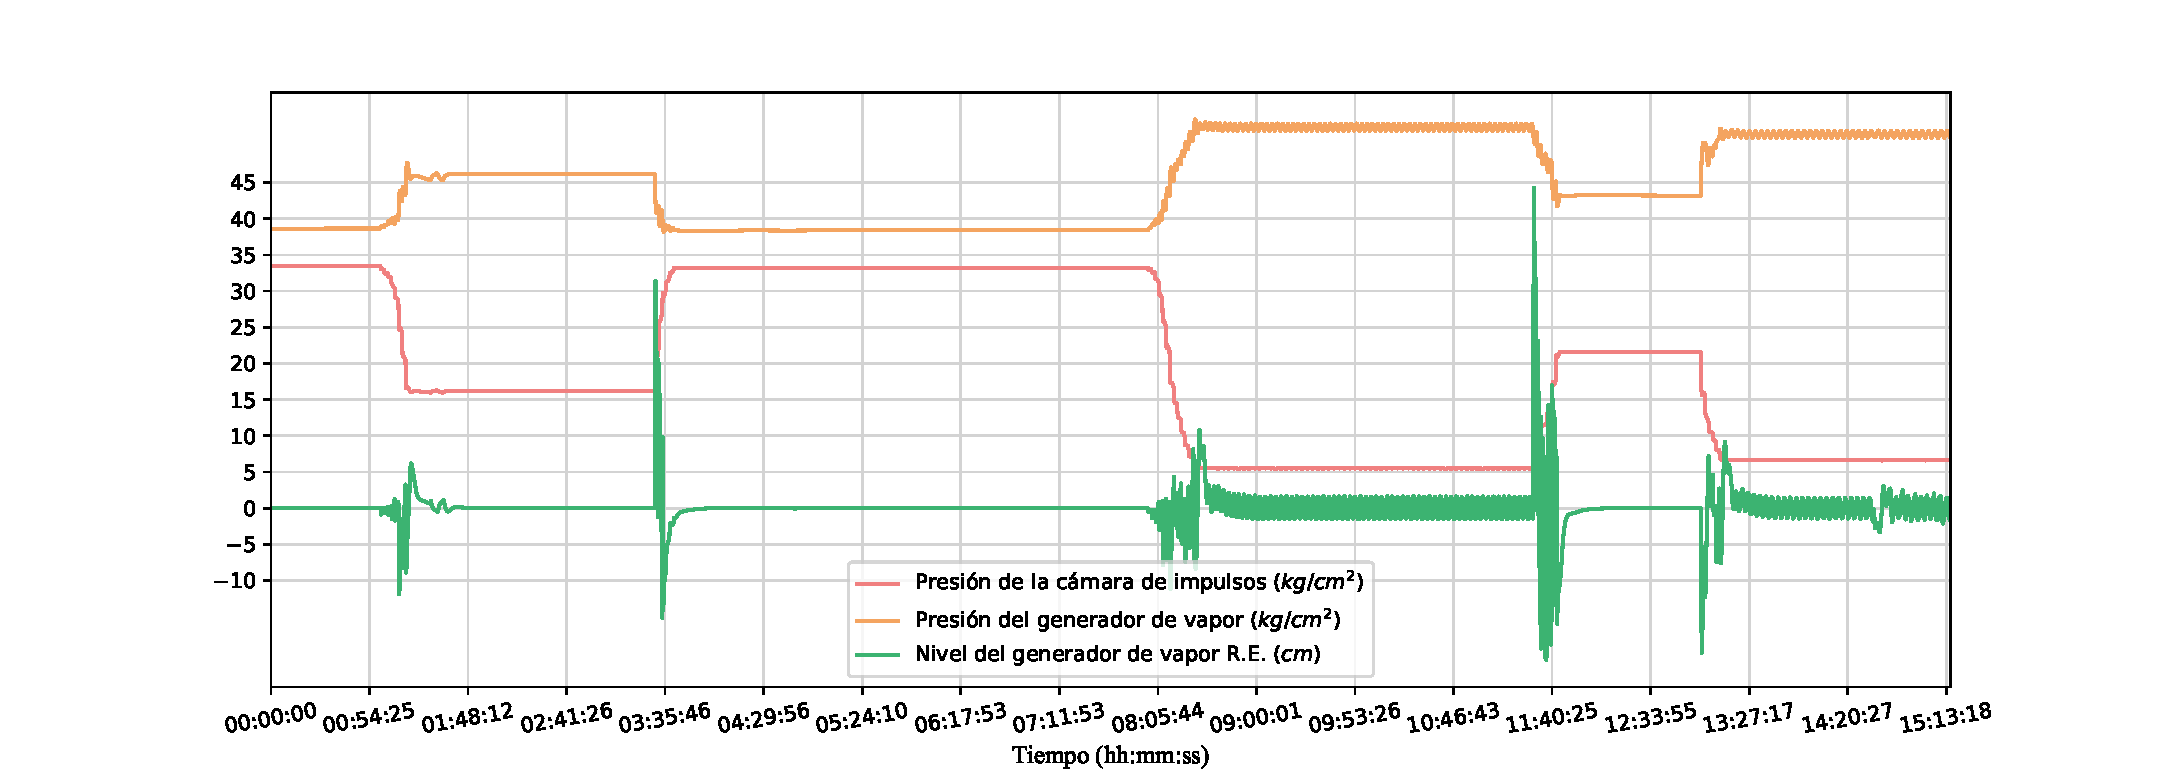
\includegraphics[width=\textwidth]{content/figures/sim4_gen_vapor_camara_imp.pdf}
  \caption{Propiedades del generador de vapor y de la cámara de impulsos.}
  \label{fig:sim4_gen_vapor_camara_imp}
\end{figure}

\begin{figure}[!h]
  \centering
  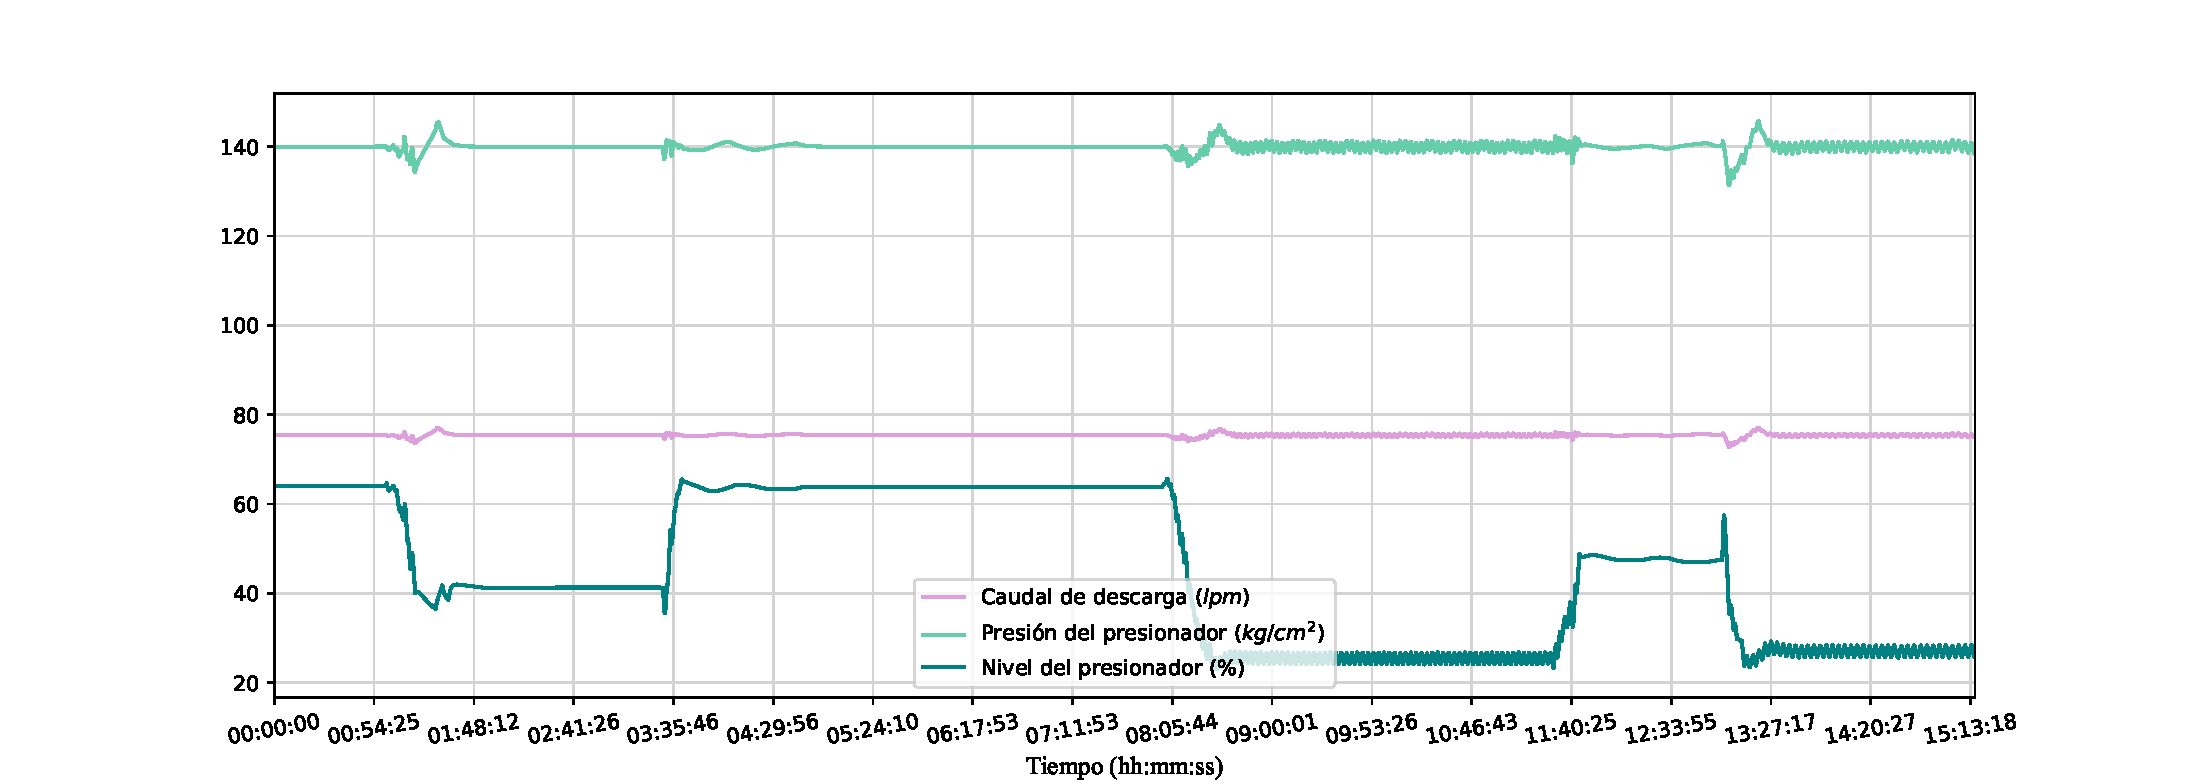
\includegraphics[width=\textwidth]{content/figures/sim4_presionador.pdf}
  \caption{Propiedades del presionador.}
  \label{fig:sim4_presionador}
\end{figure}